\documentclass{beamer}\usepackage[]{graphicx}\usepackage[]{color}
%% maxwidth is the original width if it is less than linewidth
%% otherwise use linewidth (to make sure the graphics do not exceed the margin)
\makeatletter
\def\maxwidth{ %
  \ifdim\Gin@nat@width>\linewidth
    \linewidth
  \else
    \Gin@nat@width
  \fi
}
\makeatother

\definecolor{fgcolor}{rgb}{0.345, 0.345, 0.345}
\newcommand{\hlnum}[1]{\textcolor[rgb]{0.686,0.059,0.569}{#1}}%
\newcommand{\hlstr}[1]{\textcolor[rgb]{0.192,0.494,0.8}{#1}}%
\newcommand{\hlcom}[1]{\textcolor[rgb]{0.678,0.584,0.686}{\textit{#1}}}%
\newcommand{\hlopt}[1]{\textcolor[rgb]{0,0,0}{#1}}%
\newcommand{\hlstd}[1]{\textcolor[rgb]{0.345,0.345,0.345}{#1}}%
\newcommand{\hlkwa}[1]{\textcolor[rgb]{0.161,0.373,0.58}{\textbf{#1}}}%
\newcommand{\hlkwb}[1]{\textcolor[rgb]{0.69,0.353,0.396}{#1}}%
\newcommand{\hlkwc}[1]{\textcolor[rgb]{0.333,0.667,0.333}{#1}}%
\newcommand{\hlkwd}[1]{\textcolor[rgb]{0.737,0.353,0.396}{\textbf{#1}}}%
\let\hlipl\hlkwb

\usepackage{framed}
\makeatletter
\newenvironment{kframe}{%
 \def\at@end@of@kframe{}%
 \ifinner\ifhmode%
  \def\at@end@of@kframe{\end{minipage}}%
  \begin{minipage}{\columnwidth}%
 \fi\fi%
 \def\FrameCommand##1{\hskip\@totalleftmargin \hskip-\fboxsep
 \colorbox{shadecolor}{##1}\hskip-\fboxsep
     % There is no \\@totalrightmargin, so:
     \hskip-\linewidth \hskip-\@totalleftmargin \hskip\columnwidth}%
 \MakeFramed {\advance\hsize-\width
   \@totalleftmargin\z@ \linewidth\hsize
   \@setminipage}}%
 {\par\unskip\endMakeFramed%
 \at@end@of@kframe}
\makeatother

\definecolor{shadecolor}{rgb}{.97, .97, .97}
\definecolor{messagecolor}{rgb}{0, 0, 0}
\definecolor{warningcolor}{rgb}{1, 0, 1}
\definecolor{errorcolor}{rgb}{1, 0, 0}
\newenvironment{knitrout}{}{} % an empty environment to be redefined in TeX

\usepackage{alltt}




% THEME BEAMER

\usetheme{teaching}
\usefonttheme[onlymath]{serif}
\graphicspath{{figures/}}

\usepackage{ulem}
\usepackage{multirow}
\usepackage{kbordermatrix}
\usepackage{tikz}
\usetikzlibrary{calc,shapes,backgrounds,arrows,automata,shadows,positioning}
\tikzstyle{every state}=[fill=red,draw=none,scale=0.7,font=\small,text=white]
\tikzstyle{every edge}=[-,shorten >=1pt,auto,thin,draw]
\tikzstyle{alertstate}=[fill=bleu]
\usepackage[vlined]{algorithm2e}
%% Huge number of macros, among which listing for Sweave Schunk and input

\pgfdeclareimage[width=.5cm]{computer}{figures/computer.png}
\pgfdeclareimage[width=.18\textwidth]{microarray}{figures/puce}

\title{ENSAI 3A -- spécialité Sciences du vivant}

\subtitle{\huge\currentchapter\normalsize}

\institute{\scriptsize\url{http://julien.cremeriefamily.info}}

\date{\vspace{-2em}}



\AtBeginSection{
  \begin{frame}<beamer>
    \frametitle{Plan}
    \framesubtitle{\insertpart}
    \tableofcontents[currentsection,currentsubsection, subsectionstyle=show/shaded/hide, subsubsectionstyle=show/shaded/hide]  
  \end{frame}
}

\AtBeginSubsection{
  \begin{frame}<beamer>
    \frametitle{Plan}
    \framesubtitle{\insertpart}
    \tableofcontents[currentsection,currentsubsection, subsectionstyle=show/shaded/hide, subsubsectionstyle=show/shaded/hide]  
  \end{frame}
}

\AtBeginSubsubsection{
  \begin{frame}<beamer>
    \frametitle{Plan}
    \framesubtitle{\insertpart}
    \tableofcontents[currentsection,currentsubsection, subsectionstyle=show/shaded/hide, subsubsectionstyle=show/shaded/hide]  
  \end{frame}
}

\newcommand{\dotitlepage}{%
  \begin{frame}
    \titlepage
    \vfill

  \begin{scriptsize}
  \begin{thebibliography}{99}
  \setbeamertemplate{bibliography item}[book]
  \bibitem[ESL]{ESL}    \textcolor{black}{Trevor     Hastie,    Robert
      Tibshirani, Jerome  Friedman}, 2009.  \newblock The  Elements of
  Statistical Learning (2nd Edition).
  \bibitem[Gir]{Gir}       \textcolor{black}{Christophe       Giraud},
  \newblock High-dimensional Statistics, 2013.
  \setbeamertemplate{bibliography item}[article]
  
  \bibitem[JC]{JC} \textcolor{black}{J.C.}, manuscript d'habilitation 
  \newblock Contributions to sparse methods for complex data analysis
  \end{thebibliography}
  
  \defbeamertemplate{bibliography item}{package}{\pgfuseimage{computer}}
  \setbeamertemplate{bibliography item}[package]

  \end{scriptsize}

  \end{frame}
  %
}

\newcommand{\dotoc}{%
  \begin{frame}
    \frametitle{Plan}
    \tableofcontents[currentsection,
    sectionstyle=show/show,
    subsectionstyle=hide,subsubsectionstyle=hide]
  \end{frame}
  %
}


\def\currentchapter{Introduction aux méthodes régularisées et parcimonieuses}
\IfFileExists{upquote.sty}{\usepackage{upquote}}{}
\begin{document}

\dotitlepage

\dotoc

\section{Prérequis}


\subsection{Dérivée par rapport à un vecteur}

\begin{frame}
  \frametitle{Gradient}

  \begin{definitionf}[gradient]
    Soit $f$  une application  de $\Rset^p$  dans $\Rset$.  On appelle
    gradient de $f$ le vecteur des dérivées partielles
    \begin{equation*}
      \nabla f(\bx) = \frac{\partial }{\partial \bx} f(\bx) = \left(\frac{\partial f}{\partial x_1}, \dots, \frac{\partial f}{\partial x_p}\right)^\intercal.
    \end{equation*}
  \end{definitionf}
  
  De cette définition, on déduit  en particulier la dérivée par rapport
  à un  vecteur d'une  forme linéaire,  d'une application  linéaire et
  d'une forme quadratique.
  
\end{frame}

\begin{frame}
  \frametitle{Dérivée par rapport à un vecteur}

  \begin{proposition}[dérivée par rapport à un vecteur]
    Soit    $\bu,\bx\in\Rset^p$    et   $\bA\in\mathcal{M}_{mp}$    et
    $\bS\in\mathcal{M}_{pp}$.
    \begin{align*}
      \frac{\partial}{\partial \bx} \bu^\intercal\bx & = \bu\\
      \frac{\partial}{\partial \bx} \bA\bx & = \bA\\
      \frac{\partial}{\partial \bx} \bx^\intercal\bS\bx & = \bS\bx + \bS^\intercal \bx\\      
    \end{align*}
    Si de plus $\bS$ est symétrique, alors
    \begin{equation*}
      \frac{\partial}{\partial \bx} \bx^\intercal\bS\bx = 2 \bS\bx 
    \end{equation*}
  
\end{proposition}
  
\end{frame}

\subsection{Vecteur aléatoire Gaussien}

\begin{frame}
  \frametitle{Vecteur aléatoire, espérance et  variance-covariance}

  Soit $X = (X_1,\dots,X_p)^\intercal$ un vecteur de variables aléatoires dont la distribution est définie par la densité jointe $f(\bx) = f(x_1,\dots,x_p)$.
  
\begin{definitionf}[Espérance]
L'espérance de $X$ est le vecteur d'espérance de chaque composant:
\begin{equation*}
\E X  = \left(\E(X_1), \dots, \E(X_p) \right)^\intercal.
\end{equation*}
\end{definitionf}

\vspace{-.35cm} 

\begin{definitionf}[Variance]
  La variance de $X$ est la matrice (de variance-covariance) définie par
  \begin{equation*}
\var(X) = \only<1,3->{\E\left[(X - \E X) (X - \E X)^\intercal \right]}  
\only<2>{\begin{pmatrix}
\var (X_1) & \dots & \cov(X_1,X_j ) & \dots & \cov(X_1,X_p) \\
 \vdots &  & \vdots & & \vdots \\
\cov(X_1,X_j) & \dots & \var(X_j ) & \dots & \cov(X_j,X_p) \\
 \vdots &  & \vdots & & \vdots \\
\cov (X_1,X_p) & \dots & \cov(X_j,X_p ) & \dots & \var(X_p) \\
\end{pmatrix}}
\end{equation*}
\end{definitionf}

\vspace{-.35cm}

\begin{block}{Propriétés}<3>
Soit $\bA$ une matrice $m \times p$ de constantes, alors
\begin{equation*}
\E (\bA X) = \bA \E(X), \quad \var(\bA X) = \bA \var(X) \bA^\intercal
\end{equation*}
\end{block}
\end{frame}


\begin{frame}
  \frametitle{Vecteur gaussien}

  \begin{block}{Définition}
    Le vecteur $X\in\Rset^p$ suit une distribution normale multivariée
    de moyenne $\bmu$ et de  variance $\bSigma$ si la fonction densité
    d'une réalisation de $\bx$ est données par
\begin{equation*}    
f(\bx) = (2\pi)^{-p/2} | \bSigma|^{-1/2} \exp\left\{-\frac{1}{2}(\bx-\bmu)^\intercal \bSigma^{-1}(\bx-\bmu)\right\}.
\end{equation*}
On note $X\sim\mathcal{N}(\bmu,\bSigma)$ un vecteur gaussien de $\Rset^p$.
   \end{block} 
  
  \vfill
  
  \begin{block}{Log-vraisemblance} Soit $\bX$ la matrice $n\times p$ dont les lignes, notées $\bx_i$, sont des
    réalisation indépendantes de $X$.
    \vspace{-.5cm}
    \begin{equation*}
      \log L(\bmu,\bSigma;  \bX) = -\frac{n p}{2}\log(2\pi)
      - \frac{n}{2} \log |\bSigma| -
      \frac{1}{2}  \sum_{i=1}^n  \left( \bx_i  -  \bmu\right)^\intercal
      \bSigma^{-1} \left( \bx_i - \bmu \right)    \end{equation*}
  \end{block}

\end{frame}

\begin{frame}[fragile]
  \frametitle{Vecteur gaussien}
  \framesubtitle{Exemples bivariés}

\begin{knitrout}\scriptsize
\definecolor{shadecolor}{rgb}{0.969, 0.969, 0.969}\color{fgcolor}\begin{kframe}
\begin{alltt}
\hlkwd{library}\hlstd{(mvtnorm)}
\hlstd{mu} \hlkwb{<-} \hlkwd{c}\hlstd{(}\hlnum{3}\hlstd{,}\hlnum{3}\hlstd{)}
\hlstd{Sigma.id}   \hlkwb{<-} \hlkwd{matrix}\hlstd{(}\hlkwd{c}\hlstd{(}\hlnum{1}\hlstd{,}\hlnum{0}\hlstd{,}\hlnum{0}\hlstd{,}\hlnum{1}\hlstd{),} \hlnum{2}\hlstd{,} \hlnum{2}\hlstd{)}
\hlstd{Sigma.diag} \hlkwb{<-} \hlkwd{matrix}\hlstd{(}\hlkwd{c}\hlstd{(}\hlnum{.5}\hlstd{,}\hlnum{0}\hlstd{,}\hlnum{0}\hlstd{,}\hlnum{5}\hlstd{),} \hlnum{2}\hlstd{,} \hlnum{2}\hlstd{)}
\hlstd{Sigma.cov1} \hlkwb{<-} \hlkwd{matrix}\hlstd{(}\hlkwd{c}\hlstd{(}\hlnum{1}\hlstd{,}\hlnum{0.5}\hlstd{,}\hlnum{0.5}\hlstd{,}\hlnum{1}\hlstd{),} \hlnum{2}\hlstd{,} \hlnum{2}\hlstd{)}
\hlstd{Sigma.cov2} \hlkwb{<-} \hlkwd{matrix}\hlstd{(}\hlkwd{c}\hlstd{(}\hlnum{.5}\hlstd{,}\hlopt{-}\hlnum{0.75}\hlstd{,}\hlopt{-}\hlnum{0.75}\hlstd{,}\hlnum{3}\hlstd{),} \hlnum{2}\hlstd{,} \hlnum{2}\hlstd{)}

\hlstd{X.id}    \hlkwb{<-} \hlkwd{rmvnorm}\hlstd{(}\hlnum{1000}\hlstd{,mu,Sigma.id)}
\hlstd{X.diag}  \hlkwb{<-} \hlkwd{rmvnorm}\hlstd{(}\hlnum{1000}\hlstd{,mu,Sigma.diag)}
\hlstd{X.cov1} \hlkwb{<-} \hlkwd{rmvnorm}\hlstd{(}\hlnum{1000}\hlstd{,mu,Sigma.cov1)}
\hlstd{X.cov2} \hlkwb{<-} \hlkwd{rmvnorm}\hlstd{(}\hlnum{1000}\hlstd{,mu,Sigma.cov2)}
\end{alltt}
\end{kframe}
\end{knitrout}

\end{frame}

\begin{frame}[fragile]
  \frametitle{Vecteur gaussien}
  \framesubtitle{Exemples bivariés (I)}

\begin{knitrout}\scriptsize
\definecolor{shadecolor}{rgb}{0.969, 0.969, 0.969}\color{fgcolor}
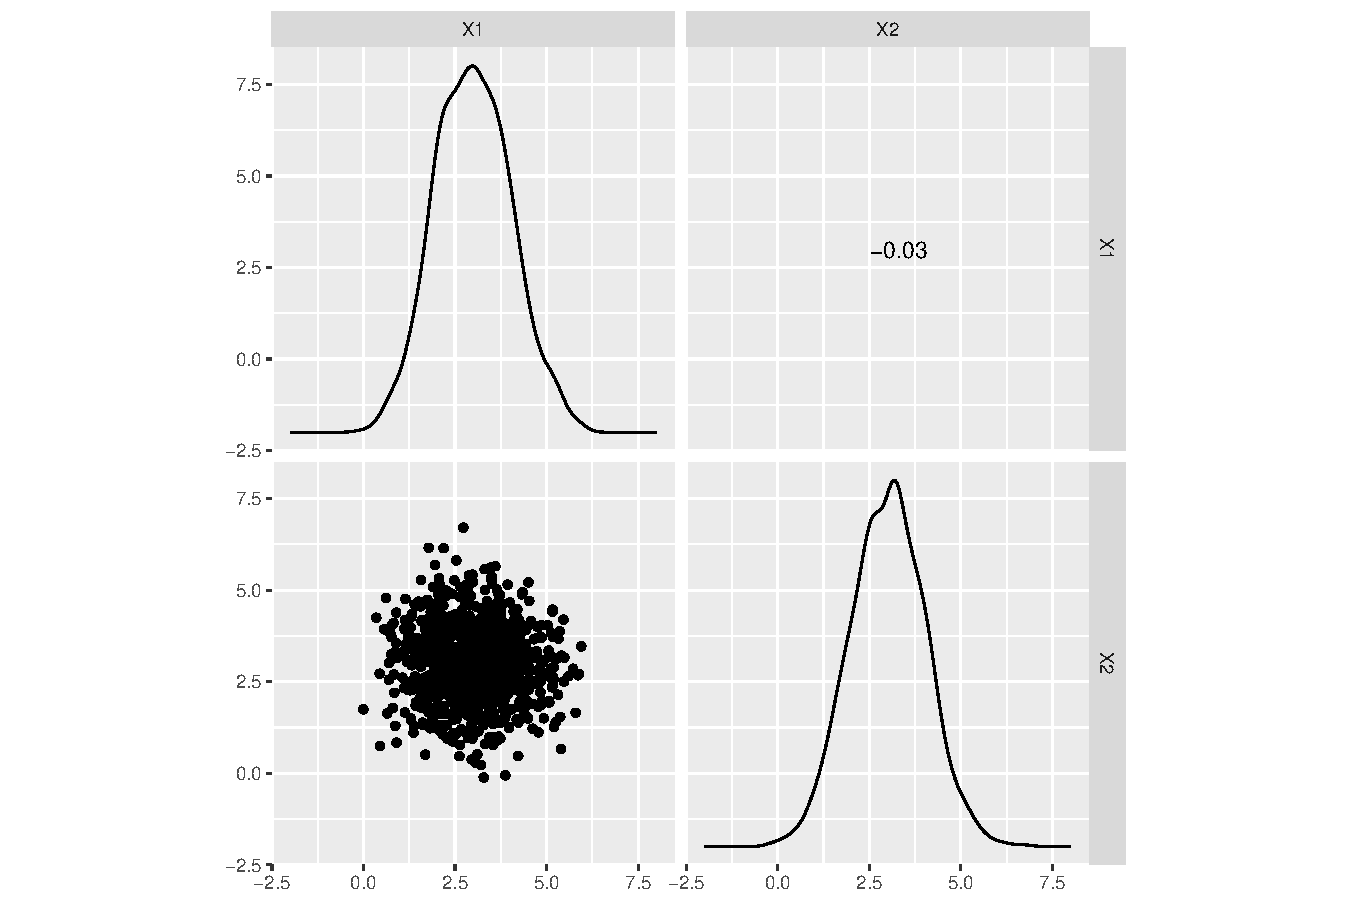
\includegraphics[width=\textwidth]{figures/algebra-unnamed-chunk-4-1} 

\end{knitrout}

\end{frame}

\begin{frame}[fragile]
  \frametitle{Vecteur gaussien}
  \framesubtitle{Exemples bivariés (II)}

\begin{knitrout}\scriptsize
\definecolor{shadecolor}{rgb}{0.969, 0.969, 0.969}\color{fgcolor}
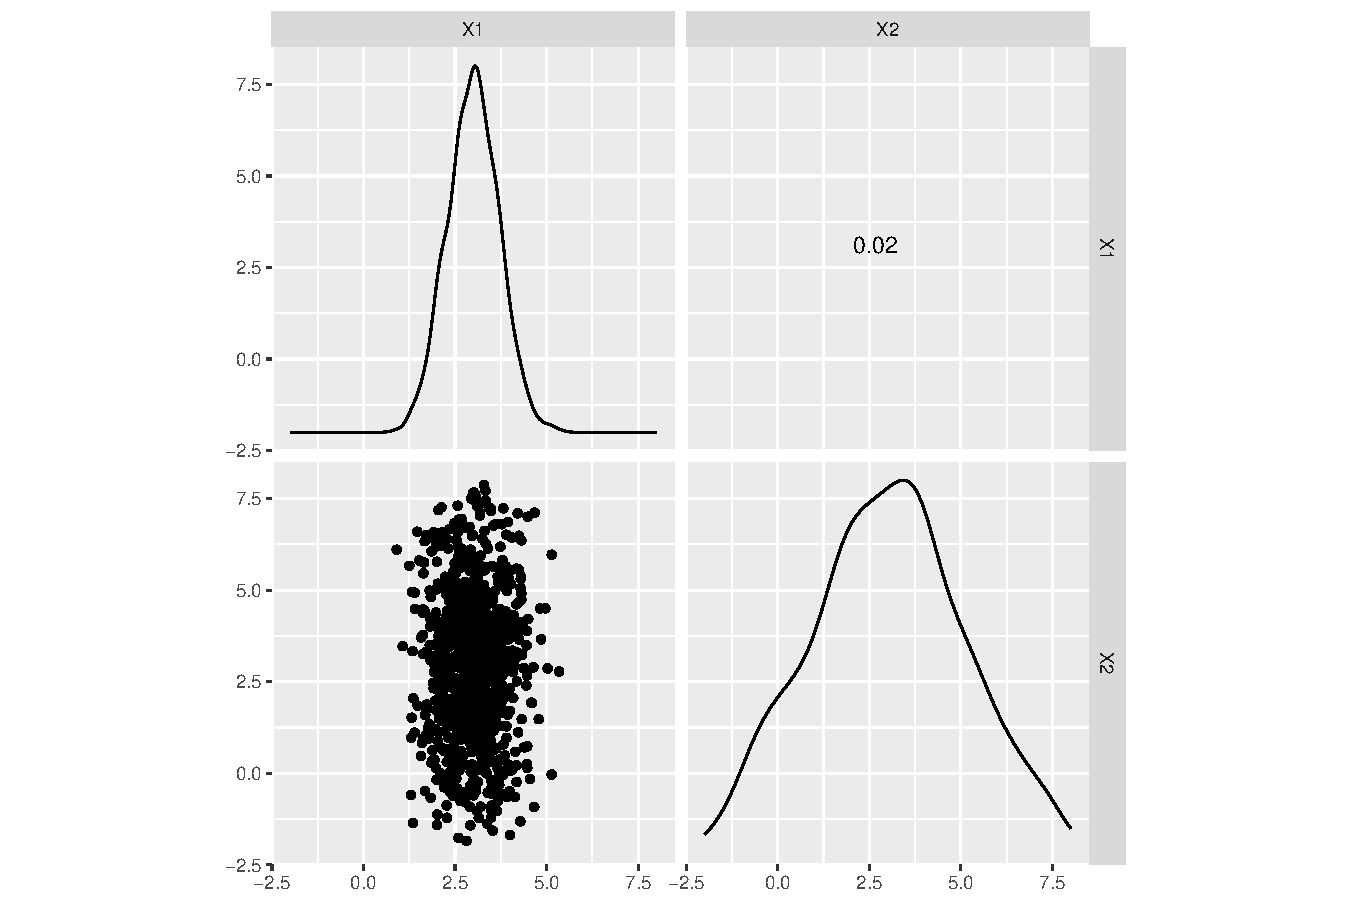
\includegraphics[width=\textwidth]{figures/algebra-unnamed-chunk-5-1} 

\end{knitrout}

\end{frame}

\begin{frame}[fragile]
  \frametitle{Vecteur gaussien}
  \framesubtitle{Exemples bivariés (III)}

\begin{knitrout}\scriptsize
\definecolor{shadecolor}{rgb}{0.969, 0.969, 0.969}\color{fgcolor}
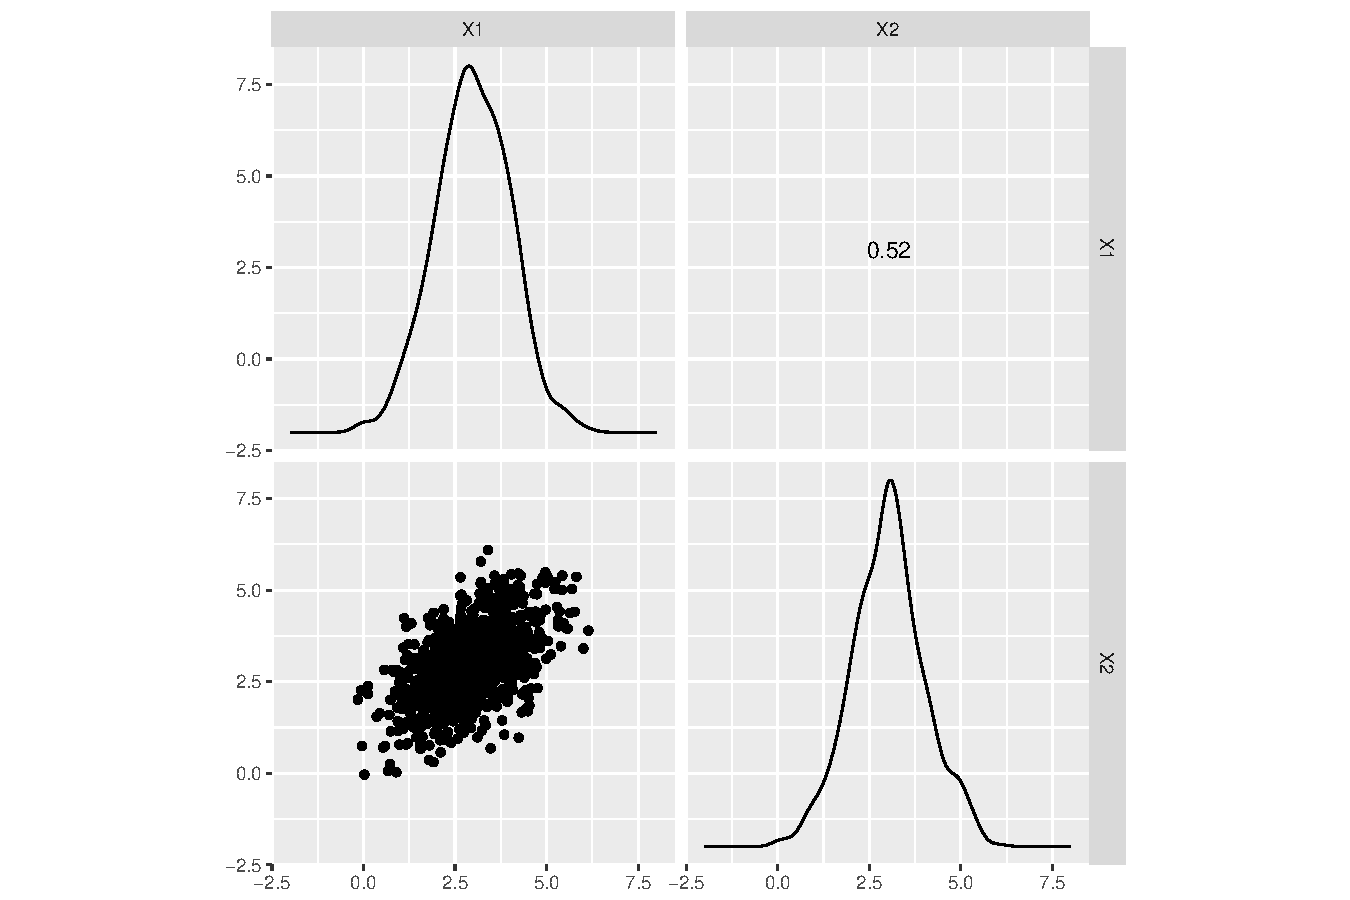
\includegraphics[width=\textwidth]{figures/algebra-unnamed-chunk-6-1} 

\end{knitrout}

\end{frame}

\begin{frame}[fragile]
  \frametitle{Vecteur gaussien}
  \framesubtitle{Exemples bivariés (IV)}

\begin{knitrout}\scriptsize
\definecolor{shadecolor}{rgb}{0.969, 0.969, 0.969}\color{fgcolor}
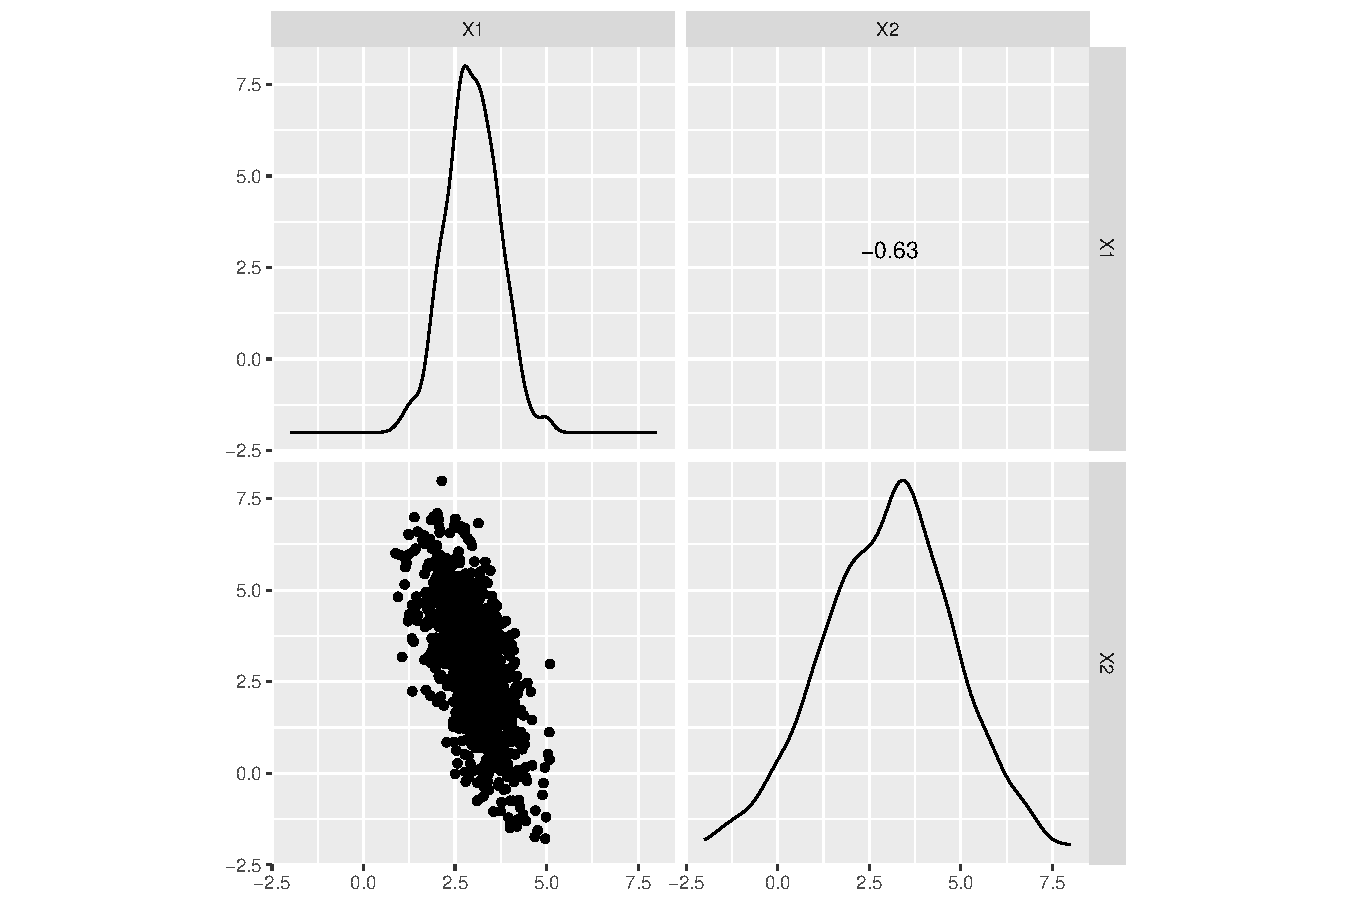
\includegraphics[width=\textwidth]{figures/algebra-unnamed-chunk-7-1} 

\end{knitrout}

\end{frame}

\begin{frame}
  \frametitle{Corrélations partielles et vecteur gaussien (I)}

  \begin{block}{Indépendance  conditionnelle: \textcolor{black}{absence  de
        \alert{\bf liens directs} entre variables}}
    $X$ et $Y$ sont indépendantes conditionnellement à $Z$ (notée $X \indep Y | Z$) ssi 
    \begin{equation*}
       \prob(X,Y|Z) = \prob(X|Z) \times \prob(Y|Z).
    \end{equation*}
  \end{block}

  \vspace{-.5cm}

   \begin{block}{Covariance/corrélation   partielle}
     C'est la covariance/corrélation une fois ôté l'effet d'une autre variable.
    \begin{gather*}
      \cov(X,Y|Z) = \cov(X,Y) - \cov(X,Z)\cov(Y,Z)/\var(Z),\\
      \rho_{XY|Z} = \frac{\rho_{XY} -
        \rho_{XZ}\rho_{YZ}}{\sqrt{1-\rho_{XZ}^2}\sqrt{1-\rho_{YZ}^2}}.
    \end{gather*}
  \end{block}

  \vspace{-.5cm}
  
  \begin{block}{Cas gaussien}
    Si $X,Y,Z$ sont jointement gaussiens, alors
    \begin{equation*}
      \alert{\cov(X,Y|Z) = 0  \Leftrightarrow \cor(X,Y|Z) = 0 \Leftrightarrow
        X \indep Y | Z.}
    \end{equation*}
  \end{block}

\end{frame}

% \begin{frame}
%   \frametitle{Partition de vecteurs gaussiens}

%   \begin{proposition}[Conditionnement]
%     Soit un vecteur gaussien et la décomposition
%     \begin{equation*}
%       Z = \begin{pmatrix}
%         Z_1 \\ Z_2
%       \end{pmatrix}  \sim   \mathcal{N}(\mathbf{0},\bSigma),   \quad
%       \bSigma = \begin{pmatrix}
%         \bSigma_{11} & \bSigma_{12} \\
%         \bSigma_{21} & \bSigma_{22} \\
%       \end{pmatrix},\quad
%       \bOmega = \bSigma^{-1} = \begin{pmatrix}
%         \bOmega_{11} & \bOmega_{12} \\
%         \bOmega_{21} & \bOmega_{22} \\
%       \end{pmatrix}.
%     \end{equation*}
%     Alors,
%     \begin{equation*}
%       Z_2|Z_1=\mathbf{z} \sim
%       \mathcal{N}\left(-\bOmega_{21}\bOmega_{22}^{-1}\mathbf{z}, \bOmega_{22}^{-1} \right)
%     \end{equation*}
%     et
%     \begin{equation*}
%       \bOmega_{22}^{-1}     =      \bSigma_{22}     -     \bSigma_{21}
%       \bSigma_{11}^{-1} \bSigma_{12}.
%     \end{equation*}
%   \end{proposition}

% \vfill
  
%   \begin{block}{Corollaire}
%     Corrélations partielles et matrice de covariance inverse sont liées
%     \begin{equation*}
%       \cor(Z_i,Z_j|Z_k, k\neq i,j) = - \frac{\Omega_{ij}}{\sqrt{\Omega_{ii}\Omega_{jj}}}
%   \end{equation*}
%   \end{block}

% \end{frame}

\subsection{Projection orthogonale}

\begin{frame}
  \frametitle{Sous espaces orthogonaux}

  \begin{definitionf}[Sous espaces vectoriels orthogonaux]
    \vspace{-.25cm}
    \begin{itemize}
    \item Les  sous espaces $V$  et $W$  sont orthogonaux si  tout les
      vecteurs de $V$ sont orthogonaux à tous les vecteurs de $W$.
    \item L'ensemble de tous les vecteurs orthogonaux à $V$ est appelé
      l'orthogonal de $V$ et est noté $V^\bot$.
    \end{itemize}    
  \end{definitionf}
  
  \begin{theoreme}
    Soit $V$ un sous-espace vectoriel de $\Rset^n$, alors tout vecteur
    de  $\Rset^n$ se  décompose  de  manière unique  en  une somme  de
    vecteurs de $V$ et de $V^\bot$.
  \end{theoreme}
  
\end{frame}

\begin{frame}
  \frametitle{Projection orthogonale}

  \begin{definitionf}[Projection orthogonale]
    Soit $V$ un sous espace de $\Rset^n$, l'application linéaire qui à
    un   vecteur   $\bu\in\Rset^n$   fait  correspondre   un   vecteur
    $\bu^\star\in V$ tel que $\bu  - \bu^\star$ appartienne à $V^\bot$
    est appelée projection orthogonale de $\bu$ dans $V$.
  \end{definitionf}
  
  \begin{definitionf}[Projecteur orthogonal et  matrice]<2-> Soit $\bX$
    une matrice $n\times p$ de plein rang telle que $n < p$.
    \begin{itemize}
    \item<2-> La projection orthogonale de $\bu\in\Rset^n$ dans l'image de $\bX$ vaut
      \begin{equation*}
        \proj{\bu}{\bX} = \underbrace{\bX \left(\bX^\intercal \bX\right)^{-1} \bX^\intercal}_{\bP_\bX}\ \bu.
      \end{equation*}
    \item<3> La projection orthogonale de $\bu\in\Rset^n$ dans le noyau de $\bX$ vaut
      \begin{equation*}
        \projorth{\bu}{\bX} = \underbrace{\left(\bI - \bX \left(\bX^\intercal \bX\right)^{-1} \bX^\intercal\right)}_{\bI - \bP_\bX} \ \bu.
      \end{equation*}       
    \end{itemize}
  \end{definitionf}
  
\end{frame}


\subsection{Régression linéaire et OLS}

\begin{frame}{Régression linéaire multiple}
  \framesubtitle{Le modèle}
  
  On suppose que la vraie relation entre $Y$ et $x$ est linéaire:  
  \[Y = \beta_0 + \sum_{j=1}^p\beta_j X_j + \varepsilon,\]

  \begin{itemize}
  \item $Y$ la variable aléatoire de réponse,
  \item $X = (X_1, \dots, X_p)$ un vecteur tel que $X_j$ peut être
      \begin{itemize}
      \item une covariable quantitative ou une transformation d'une covariable
      \item une expansion de bases (polynomiale, haart, etc.),
      \item une interaction entre covariables,
      \item un design/codage associé à une variable qualitative.
      \end{itemize}
  \item $\beta_0$ est la \alert{\bf constante} (\alert{\bf intercept})
  \item $\beta_j$ sont les \alert{\bf coefficients de régression}
  \item $\varepsilon$ est le \alert{\bf résidu} (variable aléatoire)\\
    \begin{itemize}
    \item[$\rightsquigarrow$] erreur de mesure, variabilité individuelle, facteur(s) non expliqué(s)
    \end{itemize}
  \end{itemize}

\end{frame}

\begin{frame}{Régression linéaire multiple}
  \framesubtitle{Échantillonnage et écriture matricielle}

  \begin{block}{Collecte de données / échantillonnage aléatoire}
    Soit $\{(Y_i,x_i)\}_{i=1}^n$  un $n$-échantillon  avec $Y_i\in\Rset$
    et $x_i\in\Rset^p$. On a    
    $$Y_i = \beta_0 + \sum_{j=1}^p\beta_j x_{ij} + \varepsilon_i,$$
    avec $\{\varepsilon_i\}_{i=1}^n$ indépendants, identiquement distribués.
  \end{block}
    \vspace{-.25cm}
    
  \begin{block}{Les données}
    \vspace{-.25cm}
    \begin{itemize}
    \item $\mathcal{D} = \{i:(y_i, x_i) \in \text{ l'ensemble d'entraînement}\}$,
    \item $\mathcal{T} = \{i:(y_i, x_i) \in \text{ l'ensemble de test}\}$,
    \item  $\mathbf{y}  =   (y_i)_{i\in\mathcal{D}}$,  le  vecteur  de
      réponse  dans $\mathbb{R}^{|\mathcal{D}|}$,
    \item  $\mathbf{x}_j  = (x_{ij})_{i\in\mathcal{D}}$  le
      vecteur de données pour le $j\ieme$ prédicteur dans $\mathbb{R}^{|\mathcal{D}|}$,
    \item $\mathbf{X}$ la matrice $n\times p$ dont la $j\ieme$ ligne est $\mathbf{x}_j$,
    \item $(\by_\mathcal{T},\bX_\mathcal{T})$ les données de test.
    \end{itemize}
  \end{block}

\end{frame}

\begin{frame}{Régression linéaire multiple}
  \framesubtitle{Écriture matricielle}

  \begin{align*}
    \onslide<1->{Y_i & = \beta_0 + \sum_{j=1}^p\beta_j x_{ij} + \varepsilon_i \quad i=1,\dots,n\\}
    \onslide<2->{Y & = \1_n \beta_0 + \sum_{j=1}^p\beta_j \bx_j + \bvarepsilon\\}
    \onslide<3->{Y & = (\1_n, \bx_1, \dots, \bx_p) 
      \begin{pmatrix}
        \beta_0 \\
        \beta_1 \\
        \dots \\
        \beta_p \\
      \end{pmatrix} + \bvarepsilon = 
\underbrace{\begin{pmatrix}
        1 & x_{11} & \dots & x_{1p} \\
        1 & x_{21} & \dots & x_{2p}\\
    \vdots & \vdots & \vdots & \vdots\\
        1 & x_{n1} & \dots & x_{np}\\
      \end{pmatrix}}_{\text{$\bX$, une matrice $n\times (p+1)$}} \begin{pmatrix}
        \beta_0 \\
        \beta_1 \\
        \vdots \\
        \beta_p \\
      \end{pmatrix} + 
    \begin{pmatrix}
        \varepsilon_1 \\
        \vdots \\
        \varepsilon_n \\
      \end{pmatrix}\\}
  \end{align*}
  \vspace{-.75cm}
  \begin{block}{En résumé,}<4>
    \vspace{-.5cm}
    \[Y = \bX \bbeta + \bvarepsilon.\]
  \end{block}
  
\end{frame}


\begin{frame}
  \frametitle{Estimateur des moindres carrés ordinaires}

  \begin{columns}[c]
    \begin{column}{.5\textwidth}
      \begin{block}{Géometrie}
        \begin{figure}[htbp!]
          \centering
          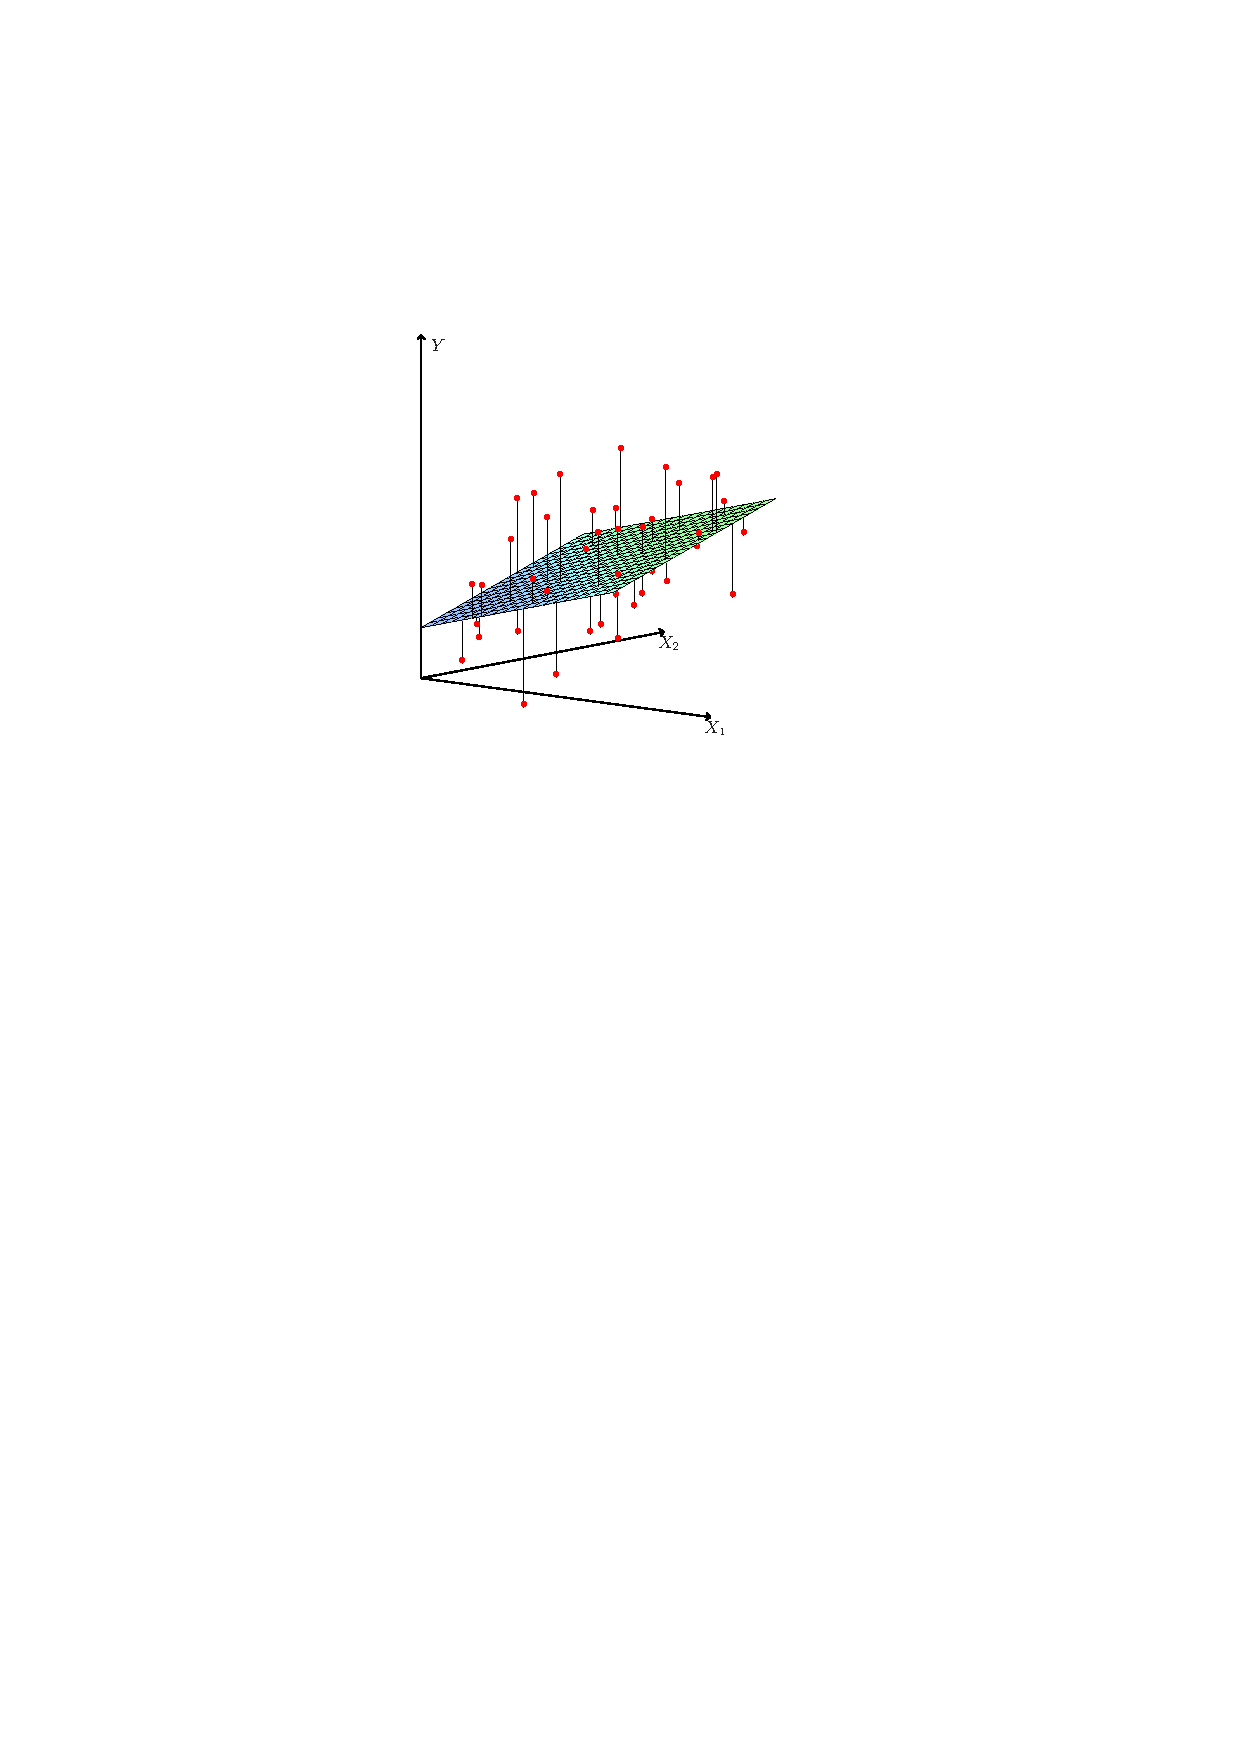
\includegraphics[width=.7\textwidth]{figures/geo_variables}
          \caption{Dans l'espace des variables $\R^{p+1}$}
        \end{figure}
      \end{block}
    \end{column}
    \begin{column}{.5\textwidth}
      \begin{block}{Critère}
        L'estimateur des moindres carrés  ordinaires minimise la somme
        des carrés des résidus (ou l'\alert{erreur d'apprentissage $\err_{\mathcal{D}}(\bbeta)$.})
        \begin{align*}
          \hatbbetaols   & =    \argmin_{\bbeta\in\mathbb{R}^{p+1}}    \|
          \mathbf{y} - \mathbf{X}\bbeta\|_2^2 \\
          & = (\mathbf{X}^\intercal\mathbf{X})^{-1}\mathbf{X}^\intercal\mathbf{y},
        \end{align*}
        Si $\bX$ est de rang plein.
      \end{block}
    \end{column}
  \end{columns}
\end{frame}

\begin{frame}
  \frametitle{MCO: géométrie dans l'espace des observations}

  \begin{block}{Valeurs ajustées}
    \begin{equation*}
    \hat{\by} = \mathbf{X}(\mathbf{X}^\intercal\mathbf{X})^{- 1}\mathbf{X}^\intercal \by = \mathbf{H}\by,
  \end{equation*}
  où $\mathbf{H}$ est la matrice de projection ou ``matrice chapeau''.
\end{block}
  \begin{columns}[c]
    \begin{column}{.5\textwidth}
      \begin{center}
        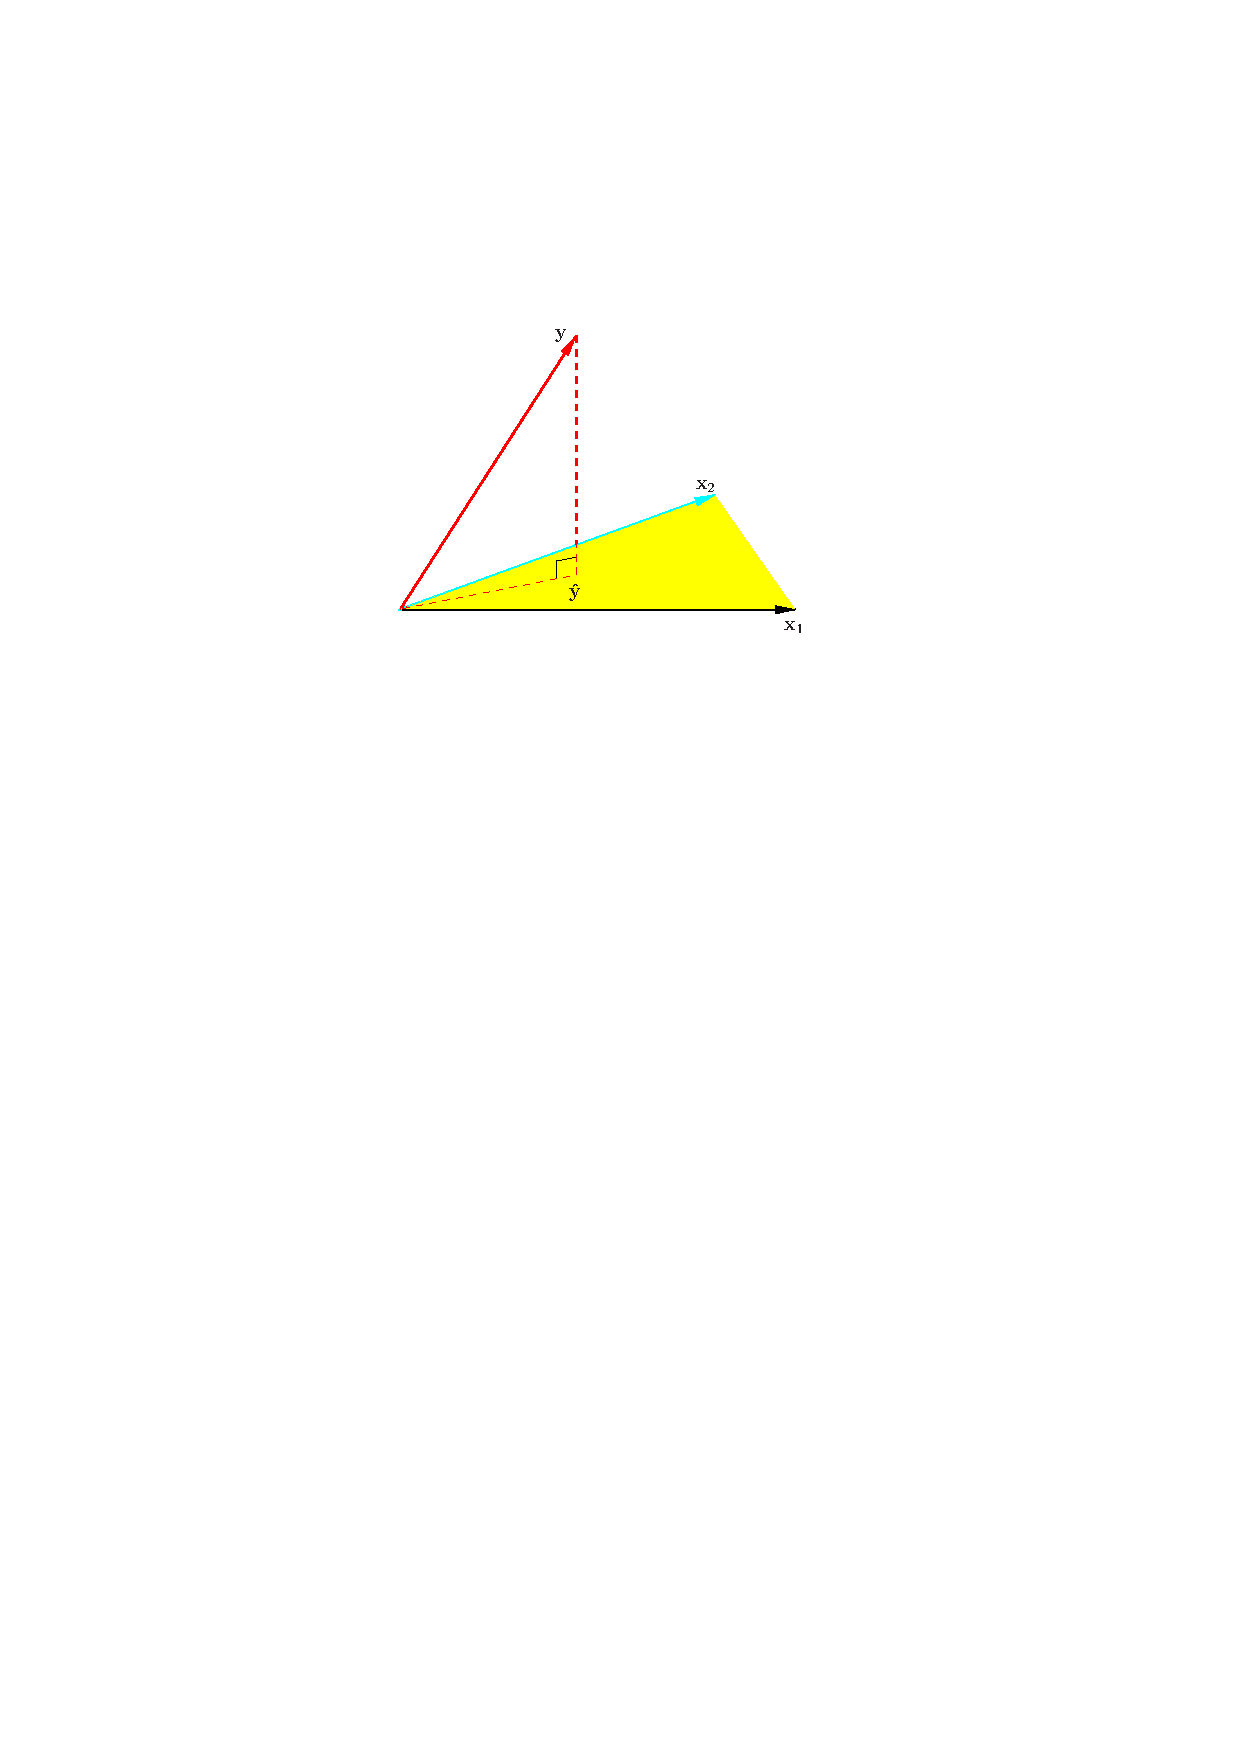
\includegraphics{figures/geo_sample}
      \end{center}
    \end{column}
    \begin{column}{.5\textwidth}
      \begin{block}{Dans l'espace des colonnes de $\bX$,}
        \begin{itemize}
        \item les $\bx_j$ engendrent un espace $n$--dimensionnel,
        \item $\hat{\by}$ est une combinaison linéaire des colonnes de
          $\bx_j$,
        \item   $\hat{\boldsymbol\varepsilon}  =   \by-\hat{\by}$  est
          orthogonal à ce sous-espace.
        \end{itemize}
      \end{block}
    \end{column}
  \end{columns}
\end{frame}

\begin{frame}{Estimation des paramètres}
   \framesubtitle{Propriétés des estimateurs}
  
   \begin{block}{Cas général}
     $\hatbbeta$ sont des estimateurs sans biais de $\beta$ de variance
     \begin{equation*}
       \var(\hatbbeta) = \sigma^2 (\bX^\intercal\bX)^{-1}.
     \end{equation*}
   \end{block}
  
   \begin{block}{Cas gaussien}
     Si les résidus sont gaussien, i.e. $\varepsilon\sim\mathcal{N}(0,\sigma^2)$, alors 
     \begin{equation*}
       \hatbbeta \sim\mathcal{N}\left(\bbeta,\sigma^2 (\bX^\intercal\bX)^{-1}\right)
     \end{equation*}
     \begin{equation*}
(\hatbbeta-\bbeta)^\intercal\frac{\bX^\intercal \bX}{\sigma^2} (\hatbbeta-\bbeta)
\sim\chi^2_{p+1}
     \end{equation*}
     \begin{equation*}
       (n-p-1) \hat\sigma^2 \sim \sigma^2\chi^2_{n-p-1}
\end{equation*}
\end{block}
 
 \end{frame}

\begin{frame}{Estimation des paramètres}
   \framesubtitle{Propriétés des estimateurs (II)}

   \begin{block}{Théorème de Gauss-Markov}
     \begin{itemize}
     \item \alert{Cas gaussien}: $\hatbbetaols$ est le
       meilleur estimateur sans biais (i.e. de variance minimale).
      
     \item \alert{Cas non gaussien}: $\hatbbetaols$ est le 
       meilleur estimateur  \alert{\bf linéaires} sans biais  (i.e. de
       variance minimale).
     \end{itemize}    
   \end{block}

   $\rightsquigarrow$ On dit que $\hatbbetaols$ est le \alert{\bf BLUE} (best linear
   unbiased estimator)
\end{frame}

\section{Motivations: les limites du modèle linéaire}


\subsection{Qualité d'un modèle de régression}

\begin{frame}
  \frametitle{Apprentissage statistique}

  \begin{block}{Problème supervisé}
    \begin{enumerate}
    \item une variable \alert{réponse} 
      \begin{itemize}
      \item soit quantitative (taille d'une tumeur, temps de survie, etc.)
      \item ou nominale (sous-type de cancer, degré d'avancement, etc.)
      \end{itemize}
    \item un ensemble de \alert{prédicteurs} 
      \begin{itemize}
      \item mesures cliniques (niveau d'expression, )
      \item âge, fumeur/non fumeur, taille, poids, etc.
      \end{itemize}
    \end{enumerate}
  \end{block}

  \vfill

  \begin{block}{Stratégie} Pour un ensemble de données
    d'entraînement, on cherche a
    \begin{enumerate}
    \item proposer un modèle,
    \item apprendre ce modèle sur l'ensemble d'entraînement,
    \item tester ce modèle sur de nouvelles observations.
    \end{enumerate}
  \end{block}

  \vfill

  $\rightsquigarrow$ \alert{Un bon modèle doit prédire correctement de
    nouvelles réponses.}

\end{frame}

\begin{frame}
  \frametitle{Modèle de régression}

  On cherche une fonction $f$ qui prédise $Y$ via $X$.

  \begin{proposition}  Le  modèle  $f(X)=\E[Y|X]$  minimise  la  perte
    quadratique, c'est-à-dire
    \begin{equation*}
      f(X)   =    \argmin_{\varphi} \mathbb{E}[(Y - \varphi(X))^2].
    \end{equation*}
    $\rightsquigarrow$ La meilleur prédiction de $Y$ à tout point $X = x$
    en terme d'espérance de l'erreur quadratique est l'espérance conditionnelle.
  \end{proposition}

  \vfill

  Cette remarque est à l'origine des modèles de régression
    \begin{equation*}
      Y = f(X) + \varepsilon,
    \end{equation*}
    où
    \begin{itemize}
    \item $\varepsilon$ est un terme d'erreur additif tel que 
      $\E[\varepsilon]=0$, $\var[\varepsilon]=\sigma^2$,
    \item $f(x) = \E[Y | X = x]$ est la \alert{\bf fonction de régression}.
    \end{itemize}

\end{frame}

\begin{frame}
  \frametitle{Stratégie d'apprentissage}

  \begin{block}{Problème}
    Les  distributions  $\P(Y|X)$  et   $\P(X)$  sont  inconnues  donc
    $\E(Y|X), \err(f(X)$ inaccessibles: il faut les \alert{\bf estimer}.
  \end{block}

  \vfill

  \begin{block}{Stratégie}
    \begin{enumerate}
    \item On se donne une famille $\mathcal{F}$ de modèles\\ 
        \onslide<2>{\textit{Pour la régression linéaire, $\mathcal{F} = \set{X^T\bbeta, \bbeta\in\Rset^p}$.}}
      \bigskip
    \item   On   ajuste   $\hat{f}\in\mathcal{F}$  sur   des   données
      d'entraînement $\mathcal{D}$\\ 
      \onslide<2>{\textit{On calcule l'estimateur des
        moindre carré $\hatbbetaols$ et $\hat f = \hat Y = \bX \hatbbetaols$}}\bigskip
    \item On estime l'erreur de prédiction $\err$  à l'aide des données test $\mathcal{T}$.
       \begin{equation*}
         \onslide<2>{\text{Par exemple, }\hat{\err}(\bX_{\mathcal{T}}\hatbbetaols) = \frac{1}{n} \left\|
         \by_{\mathcal{T}}- \bX_{\mathcal{T}} \hatbbetaols_{\mathcal{D}}\right\|^2.}
       \end{equation*}
    \end{enumerate}
  \end{block}
\end{frame}

\begin{frame}
  \frametitle{Compromis Biais/Variance}

  À un nouveau point $X=x$,
  \begin{overlayarea}{\textwidth}{\textheight}
    \begin{equation*}
      \err(\hat{f}(x))                =
      \underbrace{\sigma^2}_{\substack{\text{incompressible}\\\text{error}}}
      +
      \underbrace{\text{bias}^2(\hat{f}(x))                    +
        \var(\hat{f}(x))}_{\mathrm{MSE}(\hat{f}(x))}.
    \end{equation*}

    \begin{center}
      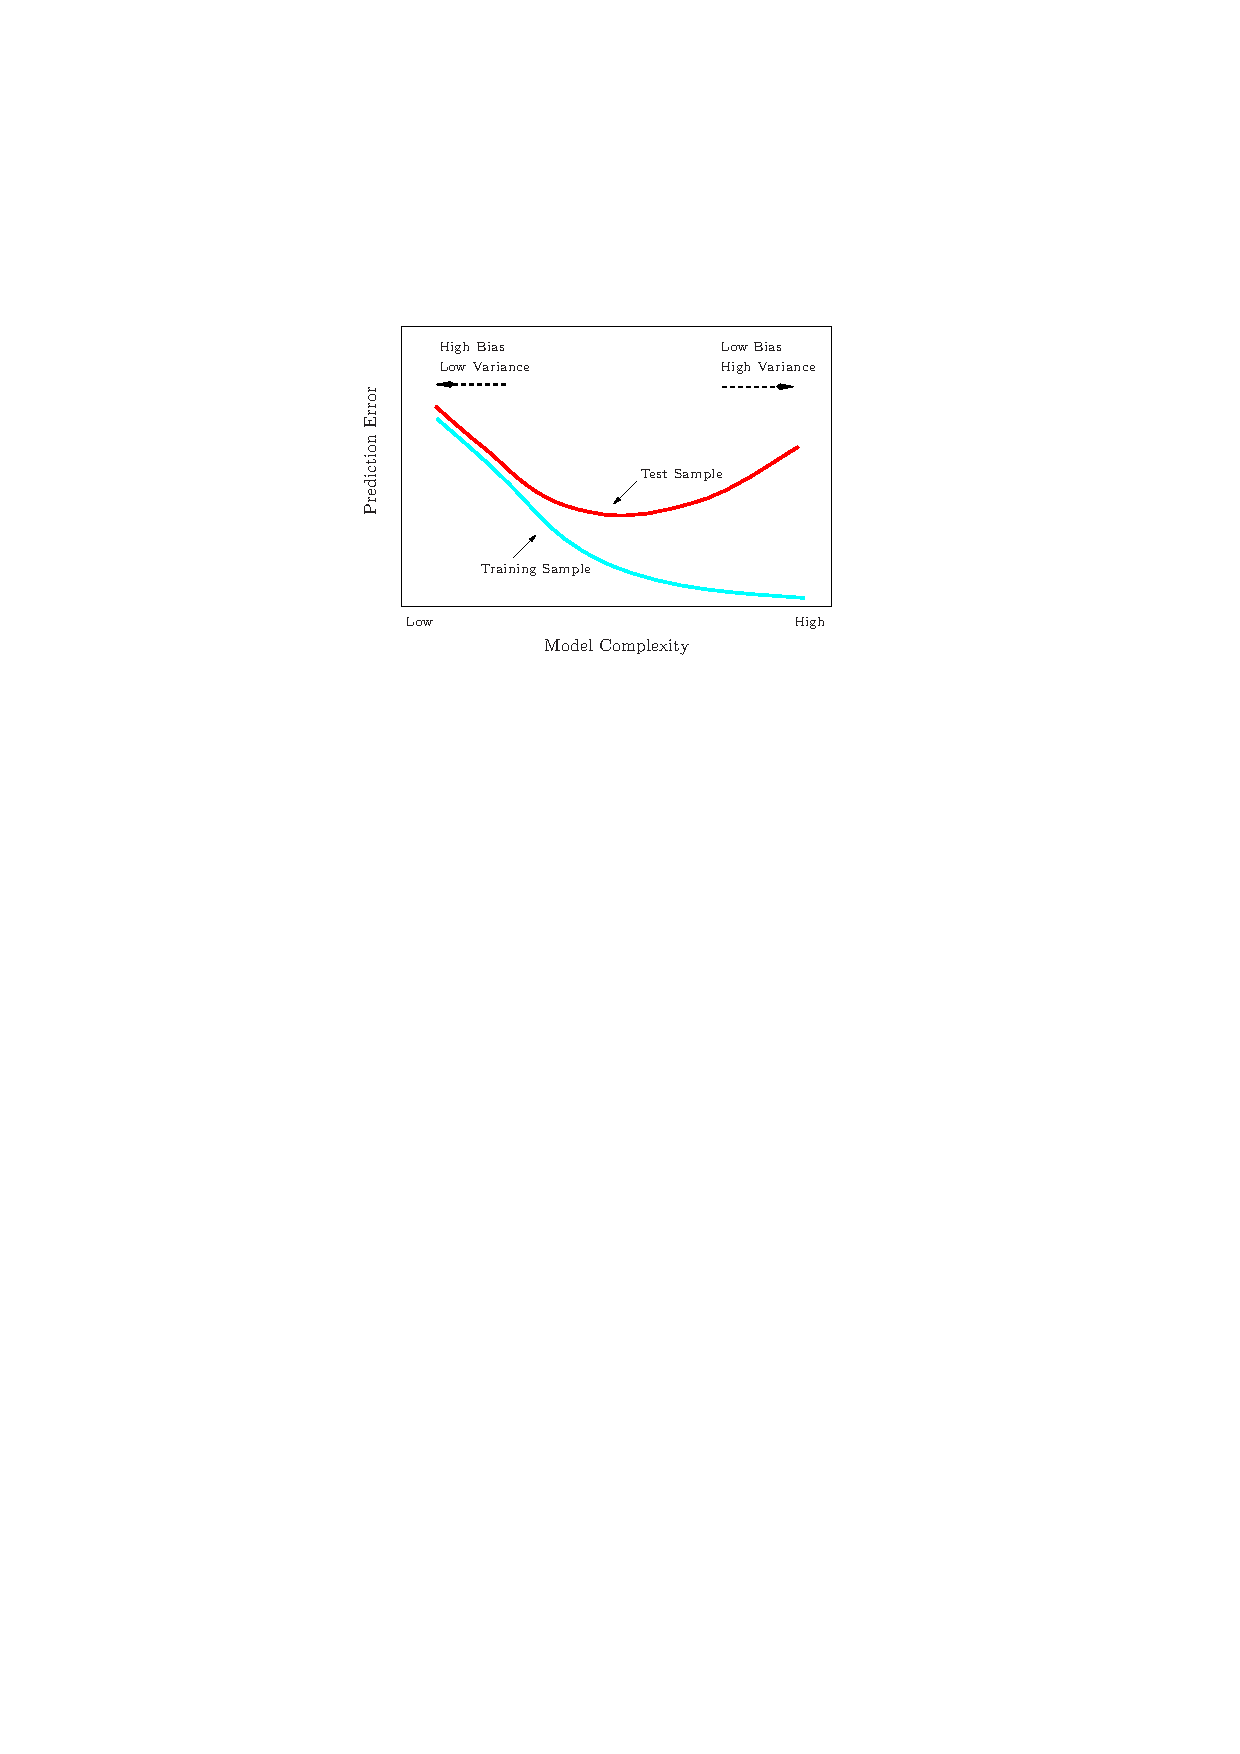
\includegraphics[width=.7\textwidth]{figures/tradeoff}
    \end{center}
  \end{overlayarea}

\end{frame}

\begin{frame}
  \frametitle{Cas de la régression linéaire}

  \begin{block}{Erreur de prédiction}
    On peut montrer pour $\bX$ fixé que 
   \begin{equation*}
      \hat{\mathrm{err}}(\bX \hatbbetaols)  = \sigma^2 \frac{(p+1)}{n} + \sigma^2.
    \end{equation*}
  \end{block}
  \vfill  
  
  \begin{block}{Thérorème de Gauss-Markov}
    $\hat  Y  = X^\intercal  \hatbbetaols$  est  le meilleur  modèle
    (i.e. de plus faible variance)  pour les estimateurs sans biais de
    $\bbeta$.
  \end{block}
  \vfill

  $\rightsquigarrow$  Y a-t-il  des situations  où l'on  a
    intérêt à utiliser un \alert{\bf estimateur biaisé de plus faible variance} ?
\end{frame}

%%% Local Variables:
%%% mode: latex
%%% TeX-master: "slides.tex"
%%% End:


\subsection{Colinéarité entre prédicteurs et OLS}

\begin{frame}
  \frametitle{OLS et colinéarité: Gram-Schmidt (I)}
  \framesubtitle{Régression par orthogonalisations successives}

  \begin{columns}[c]
    \begin{column}{.45\textwidth}
      \hspace{1cm}\begin{block}{Algorithme de Gram-Schmidt}
        \begin{scriptsize}
          \begin{algorithm}[H]
            \SetSideCommentLeft
          \DontPrintSemicolon
          \nlset{S0} \textcolor{mred}{Initialisation}\\
          $\bz_0\leftarrow \bx_0 (=\b1_{p}); $

          \BlankLine
          \nlset{S2}   \textcolor{mred}{Régression   sur  une   base
            orthonormale de $\mathrm{vect}(\bX)$}\\
          \For{$j=1,\dots,p$}{
            \For{$k=1,\dots,j-1$}{
              \textcolor{mred}{Régression de $\bx_j$ sur $\bz_k$}\\
              $\gamma_{kj}            \leftarrow            \frac{\bz_k^T
                \bx_j}{\bz_k^\intercal \bz_k}$
            }
            \textcolor{mred}{Mis à jour des résidus $\bz_j$}\\
            $\bz_j\leftarrow \bx_j - \sum_{\ell=0}^{j-1} \gamma_{\ell k} \bz_{\ell-1}$
          }
          \nlset{S3} \textcolor{mred}{Calcul de l'estimation $\hatbeta_p$} \\
          $\hatbeta_p \leftarrow \frac{\bz_p^\intercal \by}{\bz_p^\intercal\bz_p}$.
          \BlankLine
        \end{algorithm}
      \end{scriptsize}
    \end{block}

    \end{column}
    \begin{column}{.45\textwidth}
      \begin{figure}[htbp!]
        \centering
        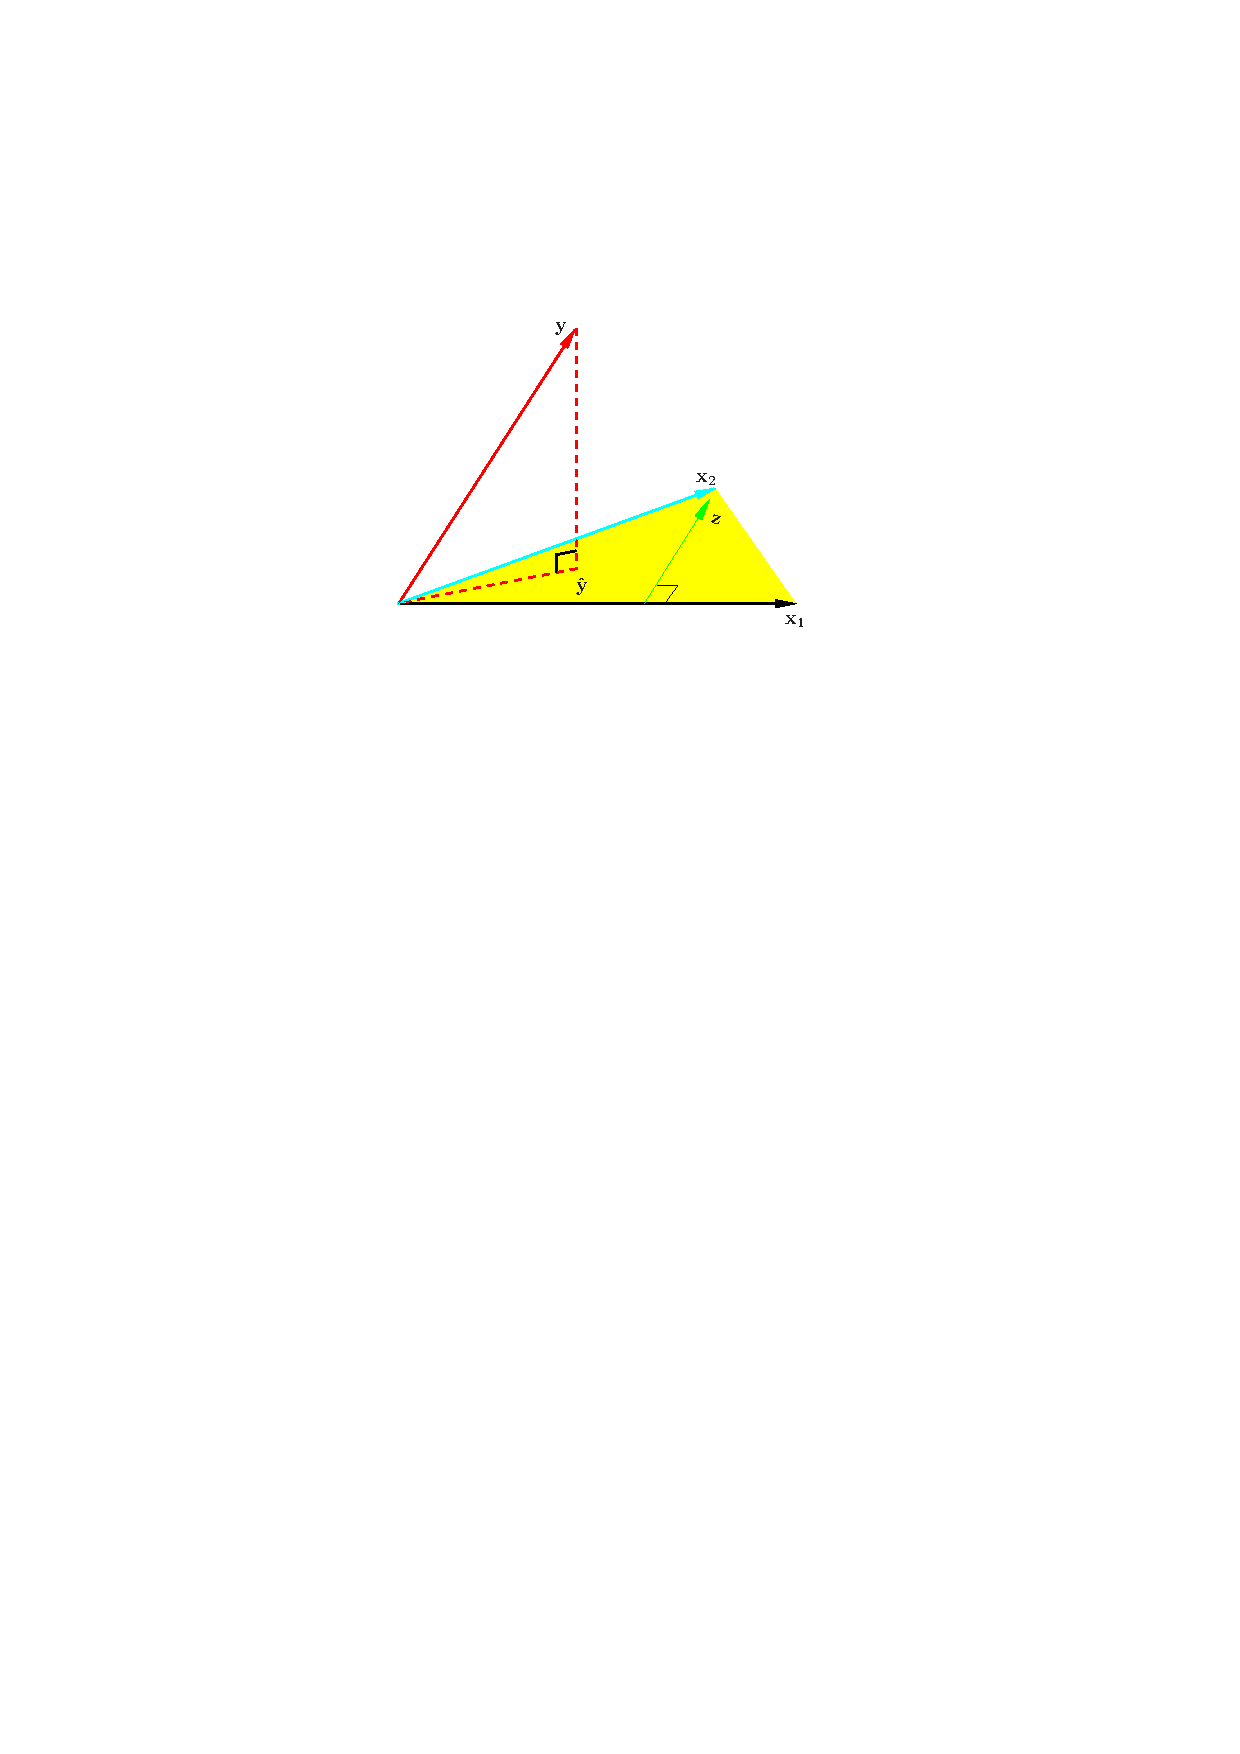
\includegraphics[width=.8\textwidth]{figures/gram_schmidt}
        \caption{Exemple avec deux prédicteurs}
    \end{figure}
    \end{column}
  \end{columns}
  \vspace{-.25cm}
  L'étape 2 peut s'écrire (avec $\bD$ diagonale telle que $\bD_{jj}=
  \bz_j^\intercal \bz_j$)
  \begin{equation*}
    \bX = \mathbf{Z}  \boldsymbol\Gamma = \mathbf{Z}\bD^{-1} \bD\boldsymbol\Gamma
    = \mathbf{Q}\mathbf{R}
    = \begin{pmatrix} \mathbf{Q}_1 & \mathbf{Q}_2\end{pmatrix}
    \begin{pmatrix} \mathbf{R}_1 \\ \mathbf{0}\end{pmatrix}    
    = \mathbf{Q}_1\mathbf{R}_1,
  \end{equation*}
  où $\mathbf{Q}_1$ est orthogonale et $\mathbf{R}_1$ triangulaire supérieure.
\end{frame}

\begin{frame}
  \frametitle{OLS et colinéarité: Gram-Schmidt (II)}
  \framesubtitle{Apportée par la factorisation QR}

  \begin{block}{Estimateur   et   prédiction   en   fonction   de   la
      factorisation QR}
    \begin{equation*}
      \hatbbetaols = \mathbf{R}_1^{-1} \mathbf{Q}_1^\intercal \by,
\qquad      \hat{\by} = \mathbf{Q}_1 \mathbf{Q}_1^\intercal \by.
    \end{equation*}

  \end{block}

  On peut permuter les colonnes de $\bX$ dans Gram-Schmidt, ainsi

  \begin{itemize}
    \item $\hatbeta_j$ est la contribution additionelle de $\bx_j$
      sur $\by$ une fois que $\bx_j$ a été ajusté sur les autres prédicteurs,
    \item La variance de $\hatbeta_p$ peut s'écrire
      \begin{equation*}
        \var(\hatbbeta_p) = \frac{\sigma^2}{\|\mathbf{z}_p\|^2_2}.
      \end{equation*}
    \end{itemize}

    $\rightsquigarrow$ prédicteurs colinéaires $\Rightarrow$ \alert{\bf mauvaise estimation de $\bbeta$}.

\end{frame}

\begin{frame}
  \frametitle{OLS et colinéarité: limite de l'interprétabilité}

  Supposons que $(X,Y)$ est un vecteur gaussien dans le
  modèle linéaire 
  
  \[Y = X^\intercal \bbeta + \varepsilon, \quad \varepsilon\sim\mathcal{N}(0,\sigma^2).\]

  Alors on peut montrer que
  
  \begin{overlayarea}{\textwidth}{\textheight}

  \onslide<1->{
    \begin{equation*}
      Y      =    \sum_{j=1}^p  X_j     \cor(X_j,Y|X_k,      k\neq      j)
      \frac{\sigma}{\sqrt{\var(X_j)}} + \varepsilon.
    \end{equation*}
    
    $\rightsquigarrow$ $\beta_j$   est   \alert{proportionnel  à   la
      corrélation partielle  entre $X_j$  et $Y$}\\
    \textit{i.e.  l'effet de $X_j$ sur $Y$ une fois les autres effets ôtés.}  
  }

  \vfill
  
  \onslide<2->{
    \begin{equation*}
      \cov(\hatbetaols_i,\hatbetaols_j) \varpropto -\cor(X_i,X_j|X_k,k\neq i,j),
    \end{equation*}
    $\rightsquigarrow$ Les prédicteurs \alert{fortement liés}
    impliquent des \alert{covariances négatives} entre les coefficients de
    régression!
  }

  \end{overlayarea}
\end{frame}


\subsection{Illustration: cancer de la prostate}






\begin{frame}[containsverbatim,allowframebreaks]
  \frametitle{Exemple: données cancer de la prostate}

  \begin{block}{97 patients atteints d'un cancer de la prostate}
    Déterminer les liens entre le niveau d'un antigène spécifique au cancer ($\mathbf{y}$) et diverses mesures cliniques.
  \end{block}

\begin{knitrout}\scriptsize
\definecolor{shadecolor}{rgb}{0.969, 0.969, 0.969}\color{fgcolor}\begin{kframe}
\begin{alltt}
\hlkwd{load}\hlstd{(}\hlstr{"prostate.rda"}\hlstd{)}
\hlkwd{dim}\hlstd{(prostate)}
\end{alltt}
\begin{verbatim}
## [1] 97 10
\end{verbatim}
\begin{alltt}
\hlkwd{print}\hlstd{(}\hlkwd{head}\hlstd{(prostate),} \hlkwc{digits}\hlstd{=}\hlnum{3}\hlstd{)}
\end{alltt}
\begin{verbatim}
##   lcavol lweight age  lbph svi   lcp gleason pgg45   lpsa train
## 1 -0.580    2.77  50 -1.39   0 -1.39       6     0 -0.431  TRUE
## 2 -0.994    3.32  58 -1.39   0 -1.39       6     0 -0.163  TRUE
## 3 -0.511    2.69  74 -1.39   0 -1.39       7    20 -0.163  TRUE
## 4 -1.204    3.28  58 -1.39   0 -1.39       6     0 -0.163  TRUE
## 5  0.751    3.43  62 -1.39   0 -1.39       6     0  0.372  TRUE
## 6 -1.050    3.23  50 -1.39   0 -1.39       6     0  0.765  TRUE
\end{verbatim}
\end{kframe}
\end{knitrout}

\begin{knitrout}\scriptsize
\definecolor{shadecolor}{rgb}{0.969, 0.969, 0.969}\color{fgcolor}
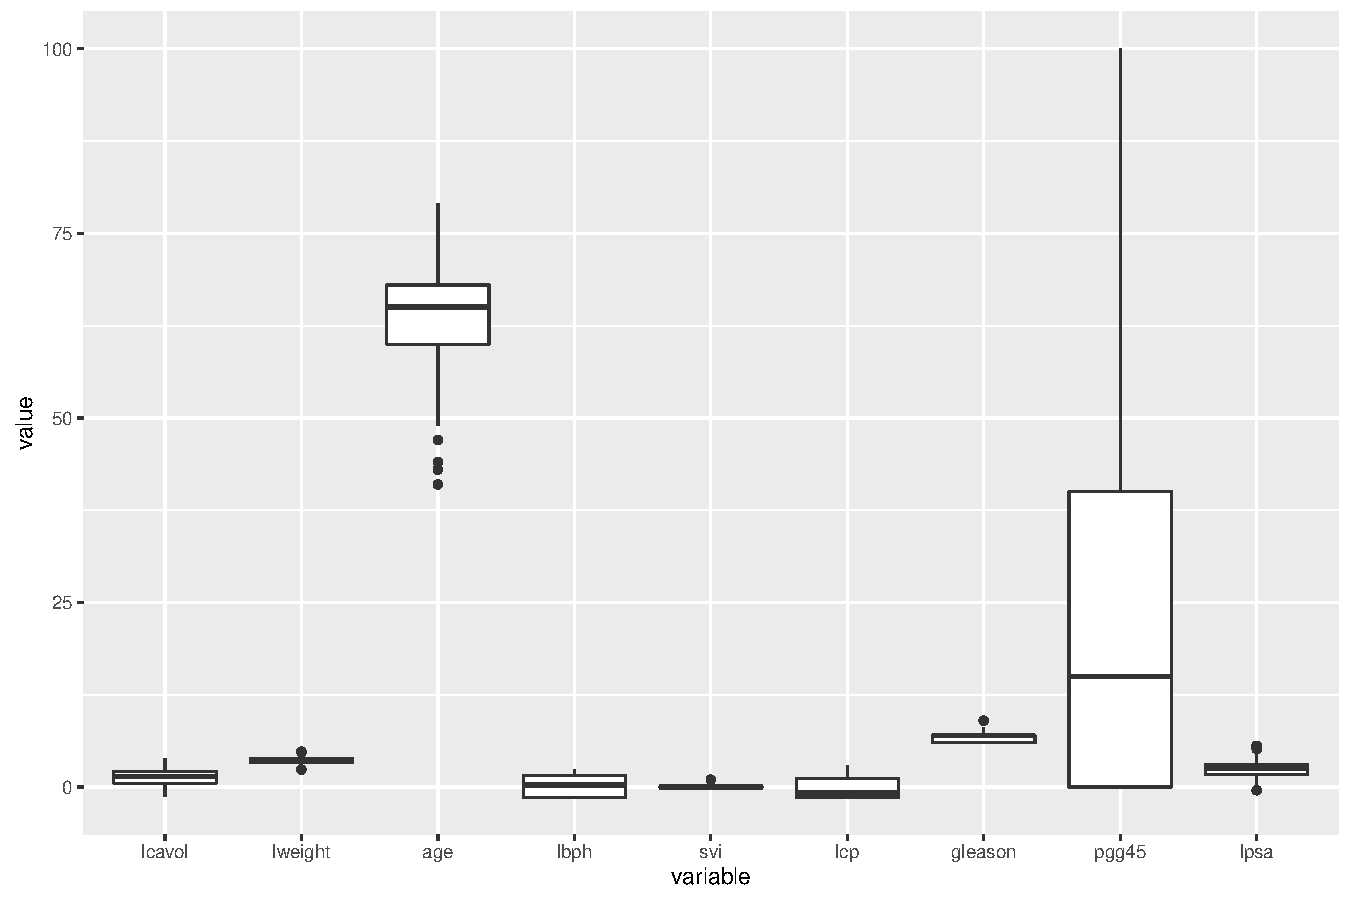
\includegraphics[width=\textwidth]{figures/olsunnamed-chunk-11-1} 

\end{knitrout}

\end{frame}

\begin{frame}[containsverbatim,allowframebreaks]
  \frametitle{Corrélations entre prédicteurs}


\begin{knitrout}\scriptsize
\definecolor{shadecolor}{rgb}{0.969, 0.969, 0.969}\color{fgcolor}\begin{kframe}
\begin{alltt}
\hlkwd{print}\hlstd{(}\hlkwd{as.dist}\hlstd{(}\hlkwd{var}\hlstd{(prostate[prostate}\hlopt{$}\hlstd{train,}\hlnum{1}\hlopt{:}\hlnum{8}\hlstd{])),}\hlkwc{digits}\hlstd{=}\hlnum{1}\hlstd{)}
\end{alltt}
\begin{verbatim}
##         lcavol lweight    age   lbph    svi    lcp gleason
## lweight  0.178                                            
## age      2.669   1.132                                    
## lbph     0.115   0.305  3.155                             
## svi      0.309   0.036  0.406 -0.086                      
## lcp      1.205   0.105  1.817 -0.182  0.395               
## gleason  0.376   0.008  1.946  0.034  0.091  0.473        
## pgg45   17.592   1.036 60.630 -1.304  5.924 27.193  15.725
\end{verbatim}
\begin{alltt}
\hlkwd{print}\hlstd{(}\hlkwd{as.dist}\hlstd{(}\hlkwd{cor}\hlstd{(prostate[prostate}\hlopt{$}\hlstd{train,}\hlnum{1}\hlopt{:}\hlnum{8}\hlstd{])),}\hlkwc{digits}\hlstd{=}\hlnum{1}\hlstd{)}
\end{alltt}
\begin{verbatim}
##         lcavol lweight   age  lbph   svi   lcp gleason
## lweight   0.30                                        
## age       0.29    0.32                                
## lbph      0.06    0.44  0.29                          
## svi       0.59    0.18  0.13 -0.14                    
## lcp       0.69    0.16  0.17 -0.09  0.67              
## gleason   0.43    0.02  0.37  0.03  0.31  0.48        
## pgg45     0.48    0.07  0.28 -0.03  0.48  0.66    0.76
\end{verbatim}
\end{kframe}
\end{knitrout}

\begin{knitrout}\scriptsize
\definecolor{shadecolor}{rgb}{0.969, 0.969, 0.969}\color{fgcolor}
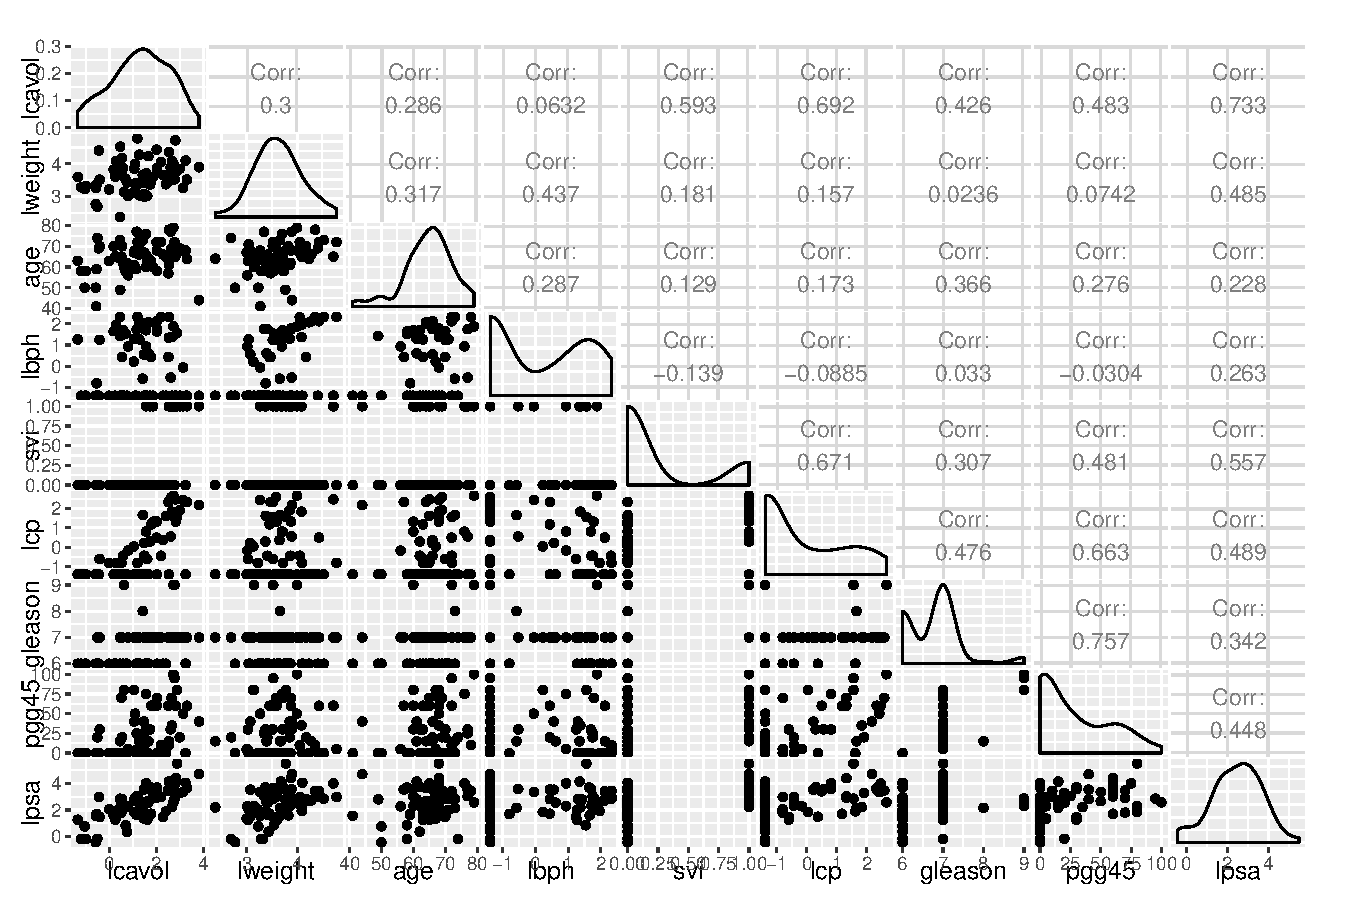
\includegraphics[width=\textwidth]{figures/olsunnamed-chunk-14-1} 

\end{knitrout}

\end{frame}

\begin{frame}[containsverbatim]
  \frametitle{Corrélations entre prédicteurs III}

\begin{knitrout}\scriptsize
\definecolor{shadecolor}{rgb}{0.969, 0.969, 0.969}\color{fgcolor}
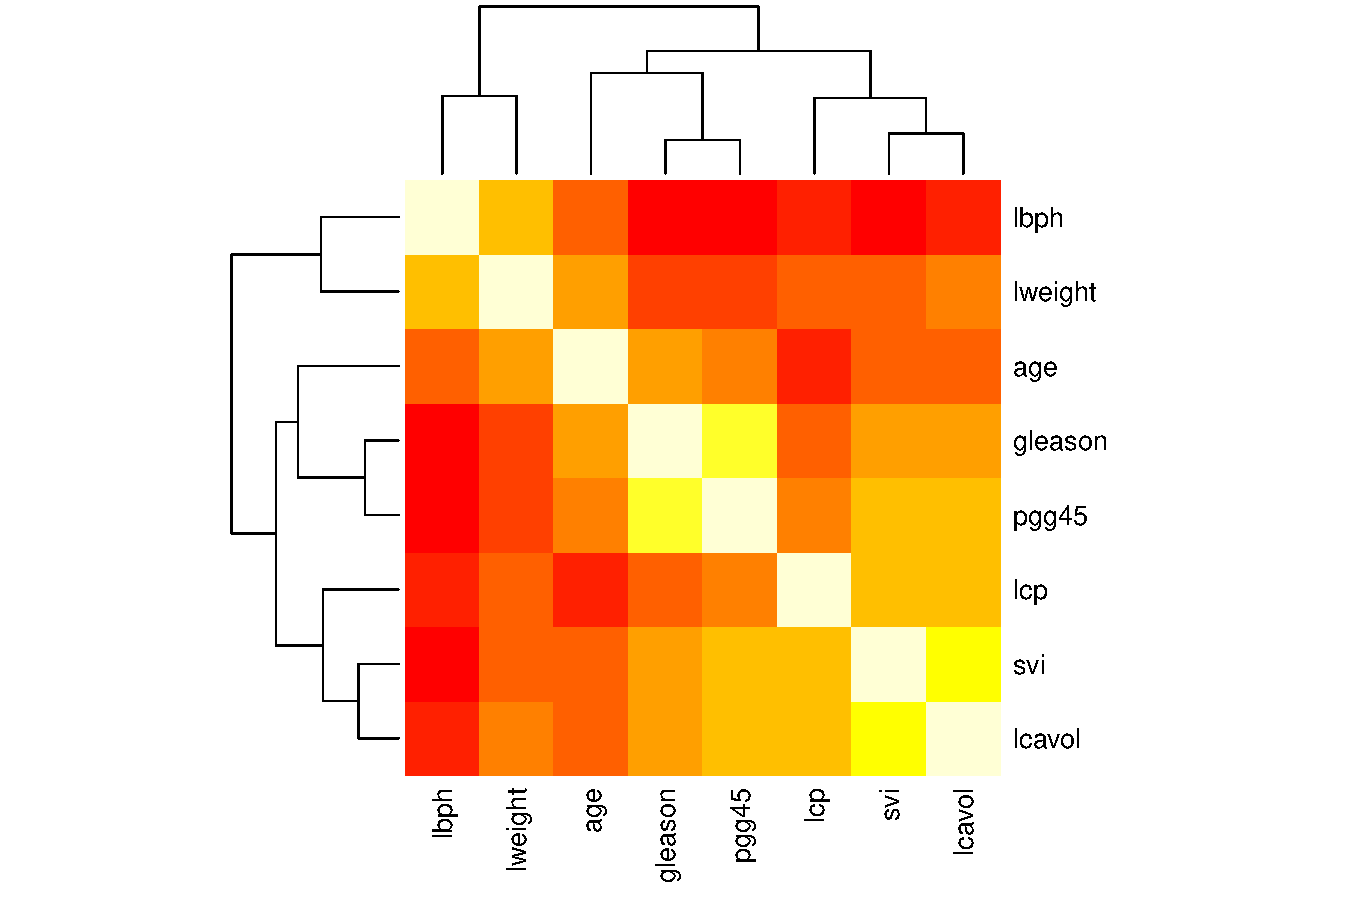
\includegraphics[width=\textwidth]{figures/olsunnamed-chunk-15-1} 

\end{knitrout}

\end{frame}


\begin{frame}[containsverbatim,allowframebreaks]
  \frametitle{Illustration des limites de l'estimateur OLS}

Pour étudier l'effet des corrélations, on ajuste un modèle avec des prédicteurs de variances comparables (normalisées).
\begin{knitrout}\scriptsize
\definecolor{shadecolor}{rgb}{0.969, 0.969, 0.969}\color{fgcolor}\begin{kframe}
\begin{alltt}
\hlstd{prostate.train} \hlkwb{<-} \hlkwd{subset}\hlstd{(prostate, train}\hlopt{==}\hlnum{TRUE}\hlstd{,} \hlopt{-}\hlstd{train)}
\hlstd{prostate.train[,} \hlnum{1}\hlopt{:}\hlnum{8}\hlstd{]} \hlkwb{<-} \hlkwd{scale}\hlstd{(prostate.train[,} \hlnum{1}\hlopt{:}\hlnum{8}\hlstd{],} \hlnum{FALSE}\hlstd{,} \hlnum{TRUE}\hlstd{)}
\hlstd{prostate.test} \hlkwb{<-} \hlkwd{subset}\hlstd{(prostate, train}\hlopt{==}\hlnum{FALSE}\hlstd{,} \hlopt{-}\hlstd{train)}
\hlstd{prostate.test[,} \hlnum{1}\hlopt{:}\hlnum{8}\hlstd{]} \hlkwb{<-} \hlkwd{scale}\hlstd{(prostate.test[,} \hlnum{1}\hlopt{:}\hlnum{8}\hlstd{],} \hlnum{FALSE}\hlstd{,} \hlnum{TRUE}\hlstd{)}
\hlstd{model.full} \hlkwb{<-} \hlkwd{lm}\hlstd{(lpsa}\hlopt{~}\hlstd{.,prostate.train)}
\end{alltt}
\end{kframe}
\end{knitrout}

   \begin{block}{Estimation de l'erreur de prédiction}
  \end{block}
\begin{knitrout}\scriptsize
\definecolor{shadecolor}{rgb}{0.969, 0.969, 0.969}\color{fgcolor}\begin{kframe}
\begin{alltt}
\hlstd{y.hat} \hlkwb{<-} \hlkwd{predict}\hlstd{(model.full,} \hlkwc{newdata}\hlstd{=prostate.test)}
\hlstd{y.test} \hlkwb{<-} \hlstd{prostate.test}\hlopt{$}\hlstd{lpsa}
\hlstd{err.ols} \hlkwb{<-} \hlkwd{mean}\hlstd{((y.test}\hlopt{-}\hlstd{y.hat)}\hlopt{^}\hlnum{2}\hlstd{)}
\hlkwd{print}\hlstd{(err.ols)}
\end{alltt}
\begin{verbatim}
## [1] 0.5221043
\end{verbatim}
\end{kframe}
\end{knitrout}

\begin{knitrout}\tiny
\definecolor{shadecolor}{rgb}{0.969, 0.969, 0.969}\color{fgcolor}\begin{kframe}
\begin{alltt}
\hlkwd{summary}\hlstd{(model.full)}
\end{alltt}
\begin{verbatim}
## 
## Call:
## lm(formula = lpsa ~ ., data = prostate.train)
## 
## Residuals:
##      Min       1Q   Median       3Q      Max 
## -1.64870 -0.34147 -0.05424  0.44941  1.48675 
## 
## Coefficients:
##             Estimate Std. Error t value Pr(>|t|)    
## (Intercept)   0.4292     1.5536   0.276  0.78334    
## lcavol        1.0466     0.1950   5.366 1.47e-06 ***
## lweight       2.2623     0.8224   2.751  0.00792 ** 
## age          -1.2477     0.8938  -1.396  0.16806    
## lbph          0.2123     0.1032   2.056  0.04431 *  
## svi           0.3515     0.1423   2.469  0.01651 *  
## lcp          -0.2924     0.1566  -1.867  0.06697 .  
## gleason      -0.2012     1.3716  -0.147  0.88389    
## pgg45         0.3737     0.2151   1.738  0.08755 .  
## ---
## Signif. codes:  0 '***' 0.001 '**' 0.01 '*' 0.05 '.' 0.1 ' ' 1
## 
## Residual standard error: 0.7123 on 58 degrees of freedom
## Multiple R-squared:  0.6944,	Adjusted R-squared:  0.6522 
## F-statistic: 16.47 on 8 and 58 DF,  p-value: 2.042e-12
\end{verbatim}
\end{kframe}
\end{knitrout}
\end{frame}

\begin{frame}
  \frametitle{Effet de la présence de colinéarité/redondance}
  
  Certains coefficients ont une grande variance (e.g. `pgg45` et `gleason`)

  \begin{block}{Considération d'ordre statistique}
    \alert{Les variables corrélées ne sont pas bien estimées},
    \\

    \begin{itemize}
    \item  Elles portent la même information vis à vis de la réponse.
    \item  Rappel:  $\cov(\hatbbeta_i,\hatbbeta_j)  \varpropto  - \cor(X_i,X_j|X_k,k\neq i,j)$.
    \end{itemize}

  \end{block}

  \vfill

  \begin{block}{Considération d'ordre numérique}
    \alert{Les variables corrélées induisent un mauvais conditionnement de $\bX^T\bX$},

    \begin{itemize}
    \item       Rappel:  $\var(\hatbbetaols_p)       = \frac{\sigma^2}{\|\mathbf{z}_p\|}$ dans la procédure de   Gram-Schmidt.

    \item l'OLS ne peut pas être calculé en présence de variables redondantes dans 
      $\bX$ \alert{ou quand  $n<p$}.
    \end{itemize}
  \end{block}

$\rightsquigarrow$ L'interprétation devient problématique
\end{frame}


\subsection{High-dimensional setup}

\begin{frame}
  \frametitle{Definition}

  \begin{definition}  We  are in  a  high-dimensional  setup when  the
    number of observations $n$  is smaller, and sometimes much smaller,
    than the number of predictors to be estimated.
  \end{definition}

  \vfill

  Thanks to new  technologies, it is now possible  to monitor a huge
  number of feature for a single individual, e.g.

  \vfill

  \begin{example}
    \begin{itemize}
    \item Genomic data,
    \item Image processing,
    \item Networks,
    \item What about your data set?
    \end{itemize}
  \end{example}

\end{frame}

\begin{frame}[containsverbatim,allowframebreaks]
  \frametitle{Consequence}

  \begin{enumerate}
  \item High level of correlation between variables become structural
  \item Inverting the empirical correlation matrix is very problematic
    \begin{itemize}
    \item The smaller $n$, The harder the inversion.
    \item As soon as $n<p$, $\bX^T\bX$ is singular.
    \end{itemize}
  \end{enumerate}



\begin{knitrout}\scriptsize
\definecolor{shadecolor}{rgb}{0.969, 0.969, 0.969}\color{fgcolor}\begin{kframe}
\begin{alltt}
\hlstd{r.maxcor} \hlkwb{<-} \hlkwa{function}\hlstd{(}\hlkwc{n}\hlstd{,}\hlkwc{p}\hlstd{) \{}
  \hlstd{C} \hlkwb{<-} \hlkwd{cor}\hlstd{(}\hlkwd{matrix}\hlstd{(}\hlkwd{rnorm}\hlstd{(n}\hlopt{*}\hlstd{p),n,p))}
  \hlkwd{return}\hlstd{(}\hlkwd{max}\hlstd{(}\hlkwd{abs}\hlstd{(C[}\hlkwd{upper.tri}\hlstd{(C)])))}
\hlstd{\}}
\hlstd{nsimu} \hlkwb{<-} \hlnum{100}
\hlstd{n} \hlkwb{<-} \hlnum{20}
\hlstd{p20}  \hlkwb{<-} \hlkwd{replicate}\hlstd{(nsimu,}\hlkwd{r.maxcor}\hlstd{(n,}\hlnum{20}\hlstd{))}
\hlstd{p100} \hlkwb{<-} \hlkwd{replicate}\hlstd{(nsimu,}\hlkwd{r.maxcor}\hlstd{(n,}\hlnum{100}\hlstd{))}
\hlstd{p500} \hlkwb{<-} \hlkwd{replicate}\hlstd{(nsimu,}\hlkwd{r.maxcor}\hlstd{(n,}\hlnum{500}\hlstd{))}
\hlstd{res} \hlkwb{<-} \hlkwd{data.frame}\hlstd{(}\hlkwc{p} \hlstd{=} \hlkwd{rep}\hlstd{(}\hlkwd{c}\hlstd{(}\hlnum{20}\hlstd{,}\hlnum{100}\hlstd{,}\hlnum{500}\hlstd{),}\hlkwc{each}\hlstd{=nsimu),}
                  \hlkwc{max.cor} \hlstd{=} \hlkwd{c}\hlstd{(p20,p100,p500))}
\end{alltt}
\end{kframe}
\end{knitrout}


\begin{knitrout}\scriptsize
\definecolor{shadecolor}{rgb}{0.969, 0.969, 0.969}\color{fgcolor}
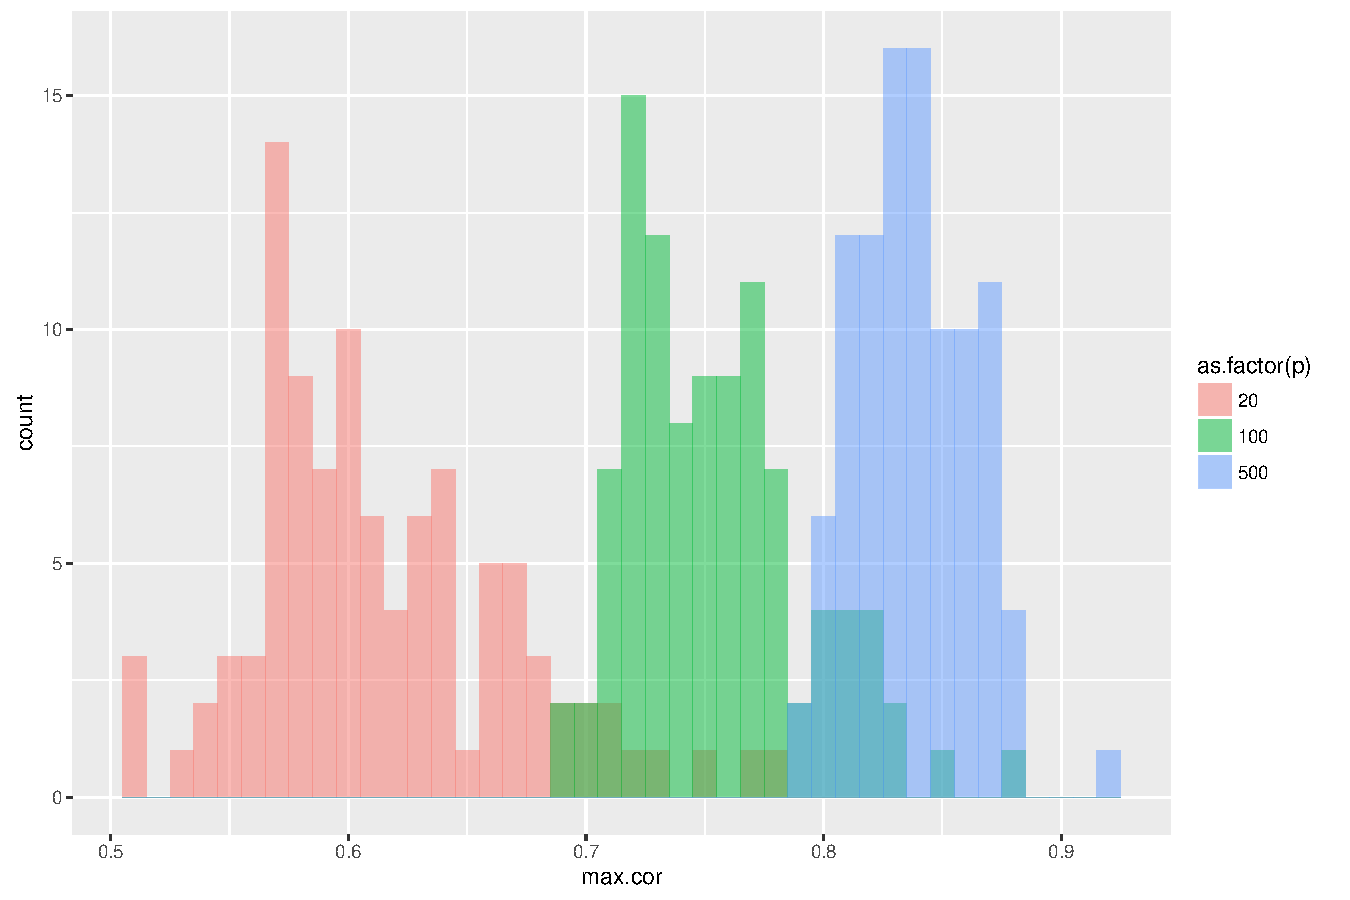
\includegraphics[width=\textwidth]{figures/highdim-unnamed-chunk-21-1} 

\end{knitrout}
\end{frame}

\begin{frame}
  \frametitle{Solutions}

  \begin{block}{Sélection de variable}
    Si le vrai modèle sous-jacent ne contient que peu de prédicteurs réellement liés à la variable réponse, on peut vouloir  \alert{sélectionner} ceux ayant un grand pouvoir prédictif. On vise ainsi
    \begin{itemize}
    \item de meilleures performances prédictives, 
    \item une meilleure interprétabilité du modèle.
    \end{itemize}
  \end{block}

  \vfill

  \begin{block}{Régularisation}<2> 

Si tous les prédicteurs ont des effet similaires sur la réponse, la sélection de prédicteurs interprétables est très difficile.

Une solution est de  \alert{\bf régulariser} le problème en  \alert{\bf contraignant} les paramètres  $\bbeta$ à vivre dans un espace approprié, de sorte à 
    \begin{itemize}
    \item rendre $\bX^T\bX$ inversible, 
    \item facilité l'interprétabilité.
    \end{itemize}
  \end{block}

\end{frame}

\begin{frame}
  \frametitle{Compromis Biais/Variance, toujours}

  Dans les deux cas, une meilleur erreur de prédiction est attendue en ajustant le \alert{compromis biais/variance} dans le modèle.

  \vfill

  \begin{center}
    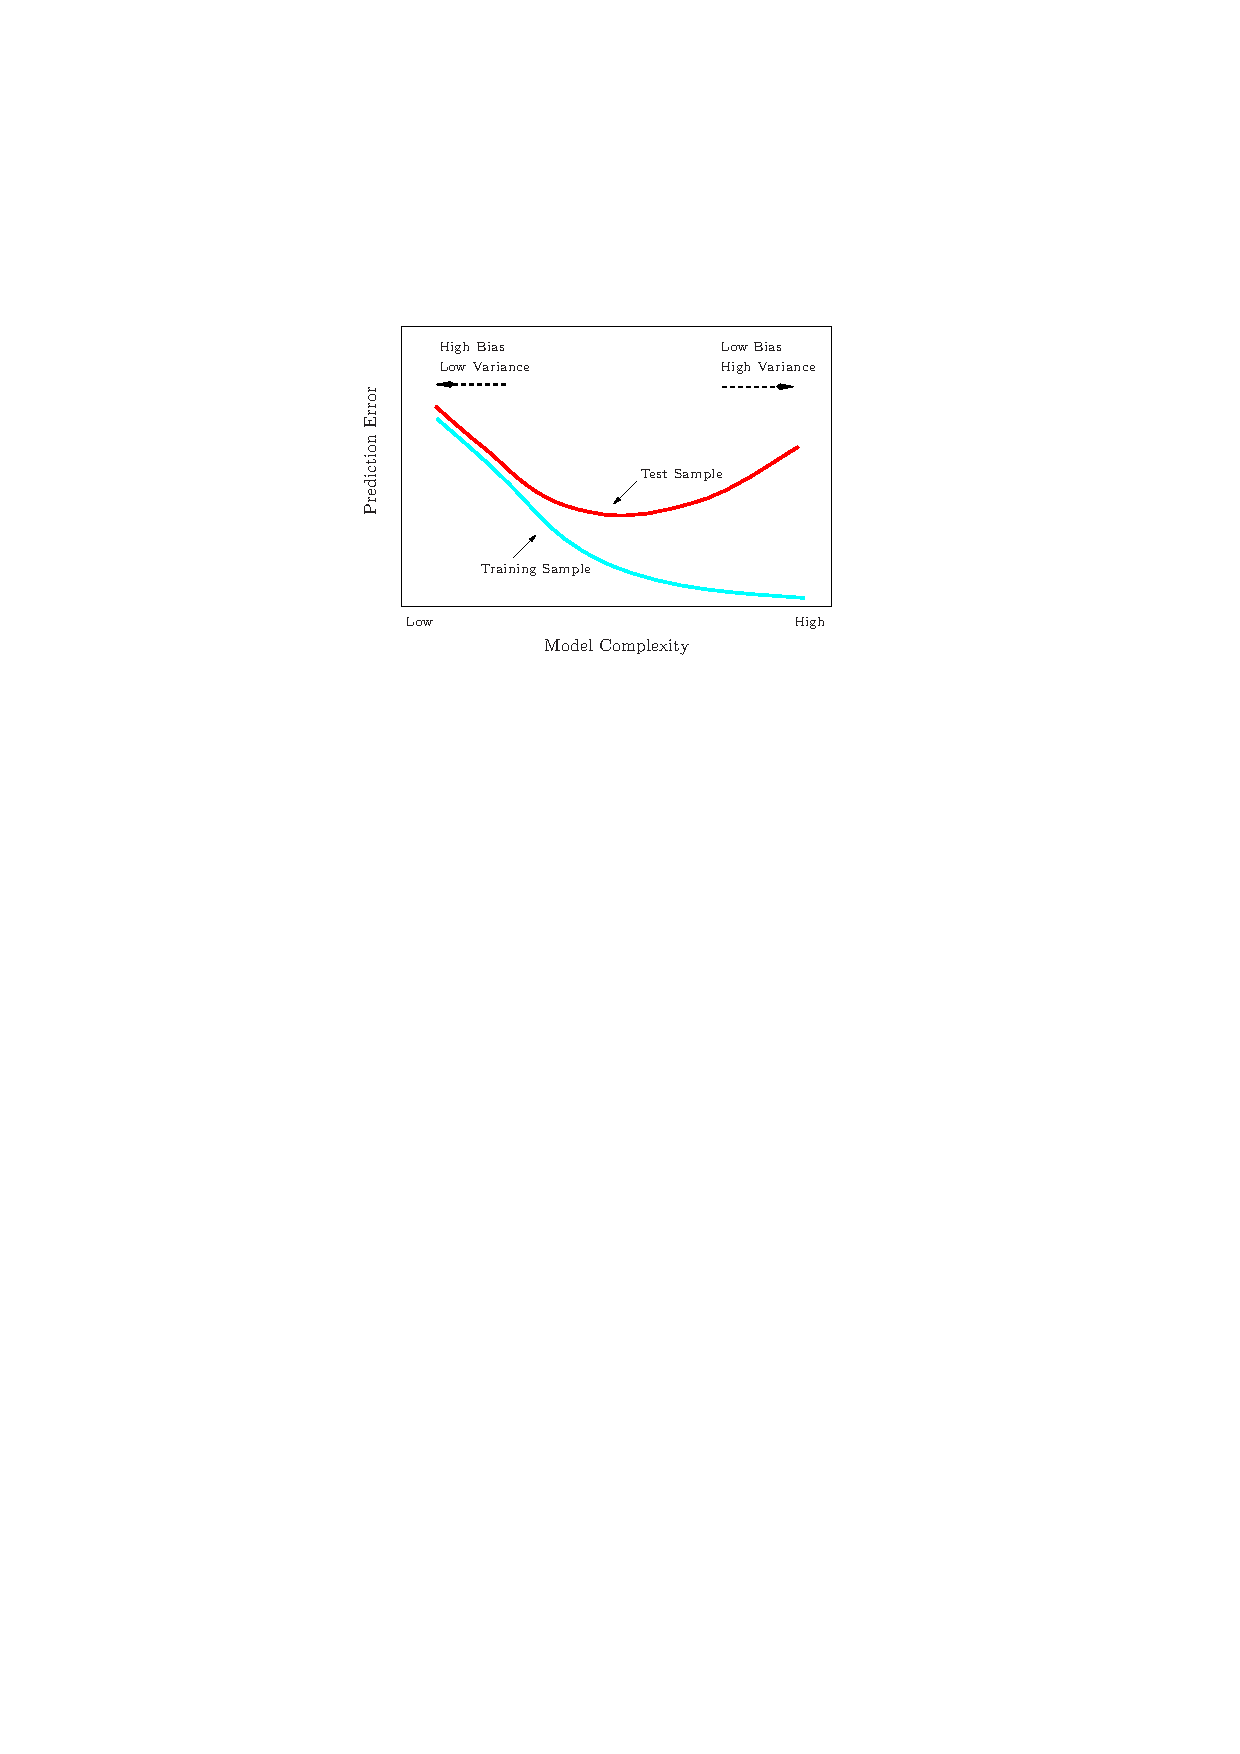
\includegraphics{figures/tradeoff}
  \end{center}

\end{frame}

\section{Sélection de variables}


\begin{frame}
  \frametitle{Sélection de variable}

  \begin{block}{Problématique}
    
  En augmentant le nombre de variables
  \begin{itemize}
  \item on intègre de plus en plus d'information dans le modèle ;
  \item on augmente le nombre de paramètres à estimer et $\var (\hat{Y}_i)\nearrow$.
  \end{itemize}  
\end{block}

  \vfill
  
  \begin{block}{Idée}
    On recherche  un (petit)  ensemble $\mathcal{S}$ de  $k$ variables
    parmi $p$ telles que
  \begin{equation*}
    Y \approx X_{\mathcal{S}}^T \hatbbeta_{\mathcal{S}}.
  \end{equation*} 
    \end{block}

  \vfill

  \begin{block}{Ingrédients}<2>
    Pour trouver un compromis, on a besoin
    \begin{enumerate}
    \item d'un \alert{critère} pour évaluer la qualité du modèle;
    \item d'un \alert{algorithme} pour déterminer les $k$ variables optimisant le critère.
    \end{enumerate}
  \end{block}

\end{frame}

\subsection{Critères de choix/comparaison de modèles}

% \begin{frame}
%   \frametitle{Erreur de prédiction}

%   \begin{block}{Estimation par l'erreur d'entraînement}
%     \alert{Attention} à ne pas estimer l'erreur par ce qu'on vient de minimiser:
%     \begin{equation*}
%       \hat{\err}_\mathcal{D}    =    \frac{1}{n_\mathrm{train}}
%       \sum_{i\in\mathcal{D}}      (y_i-       x_i^T\hatbbeta)^2      <
%       \err(X^T\hatbbeta).
%     \end{equation*}
%     $\rightsquigarrow$ On sous-estime grandement l'erreur de prédiction\dots
%   \end{block}

%   \vfill

%   \begin{block}{Estimation \og Hold-out \fg}
%     \begin{equation*}
%       \hat{\err}_\mathcal{T}    =    \frac{1}{n_\mathrm{test}}
%       \sum_{i\in\mathcal{T}}         (y_i-x_i^T\hatbbeta)^2        \approx
%       \err(X\hatbbeta).
%     \end{equation*}
%     $\rightsquigarrow$ Possible que lorsqu'on dispose d'un grand jeu de données.
%   \end{block}

% \end{frame}

% \begin{frame}
%   \frametitle{Rappel}

%     \begin{center}
%       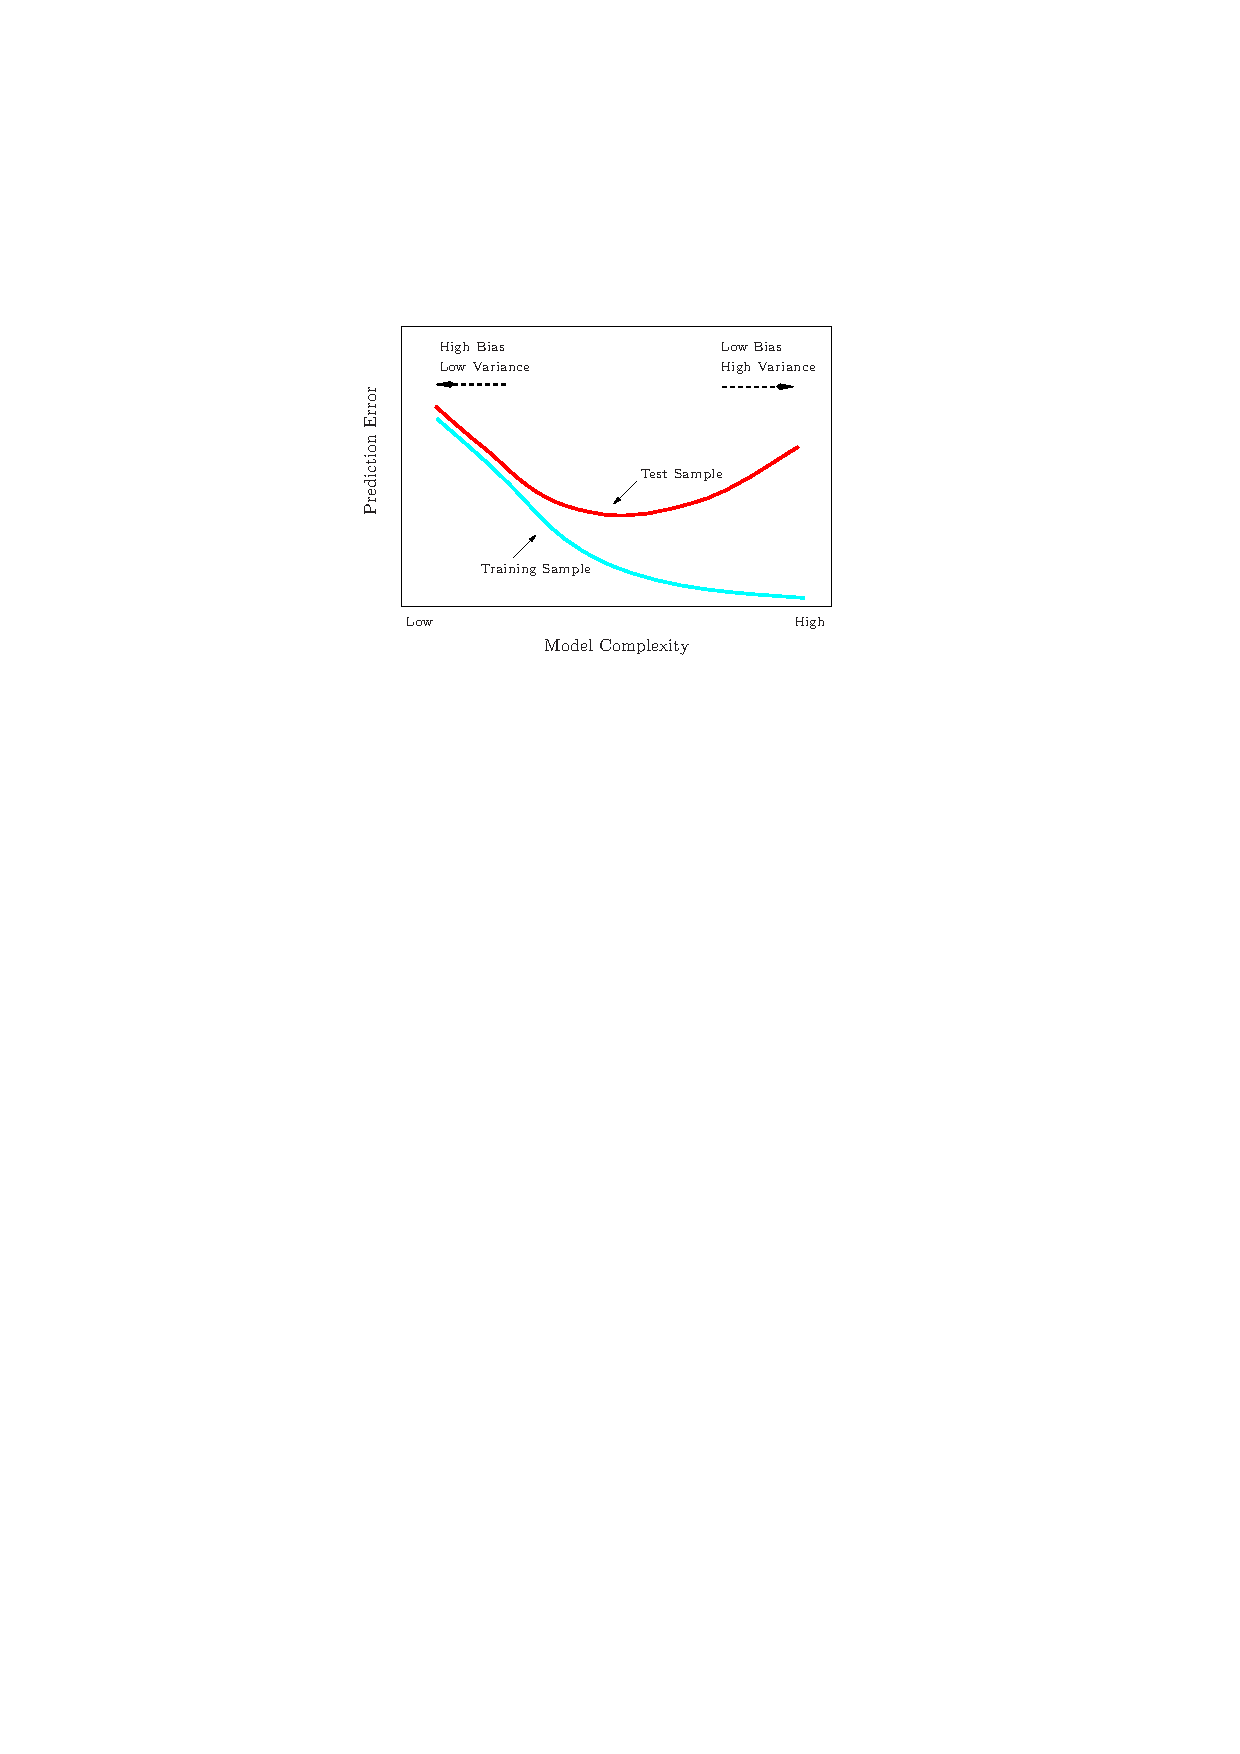
\includegraphics[width=.8\textwidth]{figures/tradeoff}
%     \end{center}

% \end{frame}

\begin{frame}
  \frametitle{Critères pénalisés}
  \framesubtitle{Principe général}
  
  \begin{block}{Idée}
    Plutôt que d'estimer l'erreur de  prédiction par l'erreur de test,
    on estime de combien  l'erreur d'entraînement sous-estime la vraie
    erreur.
  \end{block}

  \vfill
  
  \begin{block}{Forme générique des critères}
    Sans ajuster d'autres modèles, on calcule
    \begin{equation*}
      \hat{\mathrm{err}} = \mathrm{err}_{\mathcal{D}} + \mathrm{"optimisme"}.
    \end{equation*}
  \end{block}

  \vfill
  
  \begin{block}{Remarques}<2>
    \begin{itemize}
    \item beaucoup moins coûteux que la validation croisée
    \item revient à \og pénaliser \fg les modèles trop complexes.
    \end{itemize}
  \end{block}

\end{frame}

\begin{frame}
  \frametitle{Critères pénalisés}
  \framesubtitle{Les plus populaires en régression}

    Soit $k$ la dimension du modèle (le nombre de prédicteurs utilisés).
    
    \vfill

    \begin{block}{Critères  pour  le  modèle  de  régression  linéaire
        \only<1>{$\sigma$ connue}\only<2>{$\sigma$ inconnue}}
      On choisit le modèle de taille $k$ minimisant un des critères suivants.
      \begin{itemize}
      \item \alert{\bf $C_p$ de Mallows} \only<2>{$\sigma$ estimée par
          l'estimateur sans biais $\hat\sigma$}
        \[
        \only<1>{C_p= \frac{\mathrm{err}_{\mathcal{D}}}{\sigma^2} - n + 2 \frac{k}{n} }
        \only<2>{C_p= \frac{\mathrm{err}_{\mathcal{D}}}{\hat{\sigma}^2} - n + 2 \frac{k}{n} }        
        \]
    \item      \alert{\bf      Aka\"ike     Information      Criteria}
      \only<1>{équivalent au $C_p$ quand $\sigma$ est connue} \only<2>{$\sigma^2$ estimée par $\err_{\mathcal{D}}/n$}
      \[ 
      \mathrm{AIC} = - 2 \mathrm{loglik} + 2 k
      \only<1>{ = \frac{n}{\sigma^2} \mathrm{err}_{\mathcal{D}} + 2 k .}
      \only<2>{ = n \log(\mathrm{err}_{\mathcal{D}}) + 2 k .}
      \]
      
    \item \alert{\bf Bayesian Information Criterion} \only<2>{$\sigma^2$ estimée par $\err_{\mathcal{D}}/n$}
      \[ 
      \mathrm{BIC} = - 2 \mathrm{loglik} + k \log(n)
      \only<1>{ = \frac{n}{\sigma^2} \mathrm{err}_{\mathcal{D}} + k \log(n) .}
      \only<2>{ = n \log(\mathrm{err}_{\mathcal{D}}) + k \log(n) .}
      \]
    \end{itemize}
    \end{block}
  
\end{frame}

\begin{frame}{$C_p$/AIC: preuve}


  L'idéal  serait de  minimiser  l'espérance de  la
  distance  entre le  vrai  modèle $\bX  \bbeta =  \bmu$  et celui  de
  l'OLS. La distance se décompose comme suit:
\begin{align*}
\| \bmu - \bX \hatbbetaols \|^2 = & \| \by - \varepsilon - \bP_\bX \by \|^2 \\
 =& \| \by -  \hat\by \|^2 + \| \varepsilon \|^2  -2 \varepsilon^\intercal (\by -\bP_\bX\by) \\
  = & n \err_{\mathcal{D}}  + \| \varepsilon  \|^2 -2 \varepsilon^\intercal  (\bI -\bP_\bX) (\bmu + \varepsilon)\\
  = & n\err_{\mathcal{D}} - \| \varepsilon \|^2 +2 \varepsilon^\intercal \bP_\bX \varepsilon -2
\varepsilon^\intercal (\bI -\bP_\bX) \bmu
\end{align*}

En espérance, on a
\begin{itemize}
\item $\E[\| \varepsilon \|^2] = n \sigma^2$
\item $\E[\varepsilon^\intercal (\bI-\bP_\bX)\bmu]=0$
\item $\E[2 \varepsilon^\intercal \bP_\bX \varepsilon]= 2 \E[ \trace{\varepsilon^\intercal \bP_\bX
  \varepsilon}]=2 \trace{\bP_\bX}\sigma^2$
\end{itemize}

Si $k$ est la dimension de l'espace où l'on projette, on trouve
$$
\E \| \bmu - \bX \hatbbetaols \|^2 = n \err_{\mathcal{D}} - n \sigma^2 +2 k \sigma^2
$$
Il suffit alors de diviser par  $n \sigma^2$.
\end{frame}

\subsection{Algorithmes de sélection de sous-ensembles}

\begin{frame}
  \frametitle{Recherche exhaustive (best-subset)}

  \begin{block}{Algorithme}
    Pour $k=0,\dots,p$,  trouver le sous-ensemble de  $k$ variables qui
    donne le plus petit $SCR$ parmi les $2^k$ modèles.
  \end{block}
  
  \vfill
  
  \begin{block}{Propriétés}
    \begin{itemize}
    \item Peut être généralisé à d'autres critères ($R^2$, AIC, BIC\dots)
    \item Existence d'un algorithme efficace (\og Leaps and Bound \fg)
    \item impossible dès que $p>30$.
    \end{itemize}
  \end{block}
\end{frame}

\begin{frame}
  \frametitle{Sélection avant \only<1>{(Forward regression)} \only<2>{Pas à pas (Forward-stepwise)}}

  \begin{block}{Algorithme}
    \begin{itemize}
    \item[1.] Commencer avec $\mathcal{S} = \emptyset$
    \item[2.]<1> À l'étape $k$ trouver la variable qui ajoutée à $\mathcal{S}$
      donne le meilleur modèle
    \item[2'.]<2> À l'étape $k$ trouver le meilleur modèle lorsqu'une
      variable est ajoutée ou enlevée.
    \item[3] etc. jusqu'au modèle à $p$ variables
    \end{itemize}
  \end{block}
  
  \vfill
  
  \begin{block}{Propriétés}
    \begin{itemize}
    \item le meilleur modèle est compris en terme de SCR ou $R^2$,
      AIC, BIC\dots
    \item approprié lorsque $p$ est grand
    \item biais important, mais variance/complexité contrôlée.
    \item algorithme dit \og glouton \fg\ (greedy)
    \end{itemize}
  \end{block}

\end{frame}

\begin{frame}
  \frametitle{Sélection arrière}

  \begin{block}{Algorithm}
    \begin{enumerate}
    \item[1] Commencer avec le modèle plein $\mathcal{S} = \set{1,\dots,p}$
    \item[2]  À  l'étape   $k$,  enlever  la  variable   ayant  le  moins
      d'influence sur l'ajustement.
    \item[3] etc. jusqu'au modèle nul.
    \end{enumerate}
  \end{block}
  
  \vfill
  
  \begin{block}{Propriétés}
    \begin{itemize}
    \item le meilleur modèle est compris en terme de SCR ou $R^2$,
      AIC, BIC\dots
    \item ne fonctionne pas si $n <p$
    \item algorithme dit \og glouton \fg\ (greedy)
    \end{itemize}
  \end{block}

\end{frame}


\subsection{Illustration: cancer de la prostate}



\begin{frame}[containsverbatim,allowframebreaks]
  \frametitle{Recherche exhaustive}

\begin{knitrout}\scriptsize
\definecolor{shadecolor}{rgb}{0.969, 0.969, 0.969}\color{fgcolor}\begin{kframe}
\begin{alltt}
\hlkwd{library}\hlstd{(leaps)}
\end{alltt}
\end{kframe}
\end{knitrout}

On calcule tous les modèles possibles 
\begin{knitrout}\scriptsize
\definecolor{shadecolor}{rgb}{0.969, 0.969, 0.969}\color{fgcolor}\begin{kframe}
\begin{alltt}
\hlstd{out} \hlkwb{<-} \hlkwd{regsubsets}\hlstd{(lpsa} \hlopt{~} \hlstd{. ,} \hlkwc{data}\hlstd{=prostate.train,}
                  \hlkwc{nbest}\hlstd{=}\hlnum{100}\hlstd{,} \hlkwc{really.big}\hlstd{=}\hlnum{TRUE}\hlstd{)}
\hlstd{bss} \hlkwb{<-} \hlkwd{summary}\hlstd{(out)}
\end{alltt}
\end{kframe}
\end{knitrout}

Extraction de la taille et des SCR. Ajout du modèle nul (juste l'intercept)
\begin{knitrout}\scriptsize
\definecolor{shadecolor}{rgb}{0.969, 0.969, 0.969}\color{fgcolor}\begin{kframe}
\begin{alltt}
\hlstd{bss.size}  \hlkwb{<-} \hlkwd{as.numeric}\hlstd{(}\hlkwd{rownames}\hlstd{(bss}\hlopt{$}\hlstd{which))}
\hlstd{intercept} \hlkwb{<-} \hlkwd{lm}\hlstd{(lpsa} \hlopt{~} \hlnum{1}\hlstd{,} \hlkwc{data}\hlstd{=prostate)}
\hlstd{bss.best.rss}  \hlkwb{<-} \hlkwd{c}\hlstd{(}\hlkwd{sum}\hlstd{(}\hlkwd{resid}\hlstd{(intercept)}\hlopt{^}\hlnum{2}\hlstd{),} \hlkwd{tapply}\hlstd{(bss}\hlopt{$}\hlstd{rss  , bss.size, min))}
\end{alltt}
\end{kframe}
\end{knitrout}

\begin{knitrout}\scriptsize
\definecolor{shadecolor}{rgb}{0.969, 0.969, 0.969}\color{fgcolor}\begin{kframe}
\begin{alltt}
\hlkwd{plot}\hlstd{(}\hlnum{0}\hlopt{:}\hlnum{8}\hlstd{, bss.best.rss,} \hlkwc{ylim}\hlstd{=}\hlkwd{c}\hlstd{(}\hlnum{30}\hlstd{,} \hlnum{135}\hlstd{),} \hlkwc{type}\hlstd{=}\hlstr{"b"}\hlstd{,}
     \hlkwc{xlab}\hlstd{=}\hlstr{"subset size"}\hlstd{,} \hlkwc{ylab}\hlstd{=}\hlstr{"RSS"}\hlstd{,} \hlkwc{col}\hlstd{=}\hlstr{"red2"} \hlstd{)}
\hlkwd{points}\hlstd{(bss.size, bss}\hlopt{$}\hlstd{rss,} \hlkwc{pch}\hlstd{=}\hlnum{20}\hlstd{,} \hlkwc{col}\hlstd{=}\hlstr{"gray"}\hlstd{,} \hlkwc{cex}\hlstd{=}\hlnum{0.7}\hlstd{)}
\end{alltt}
\end{kframe}
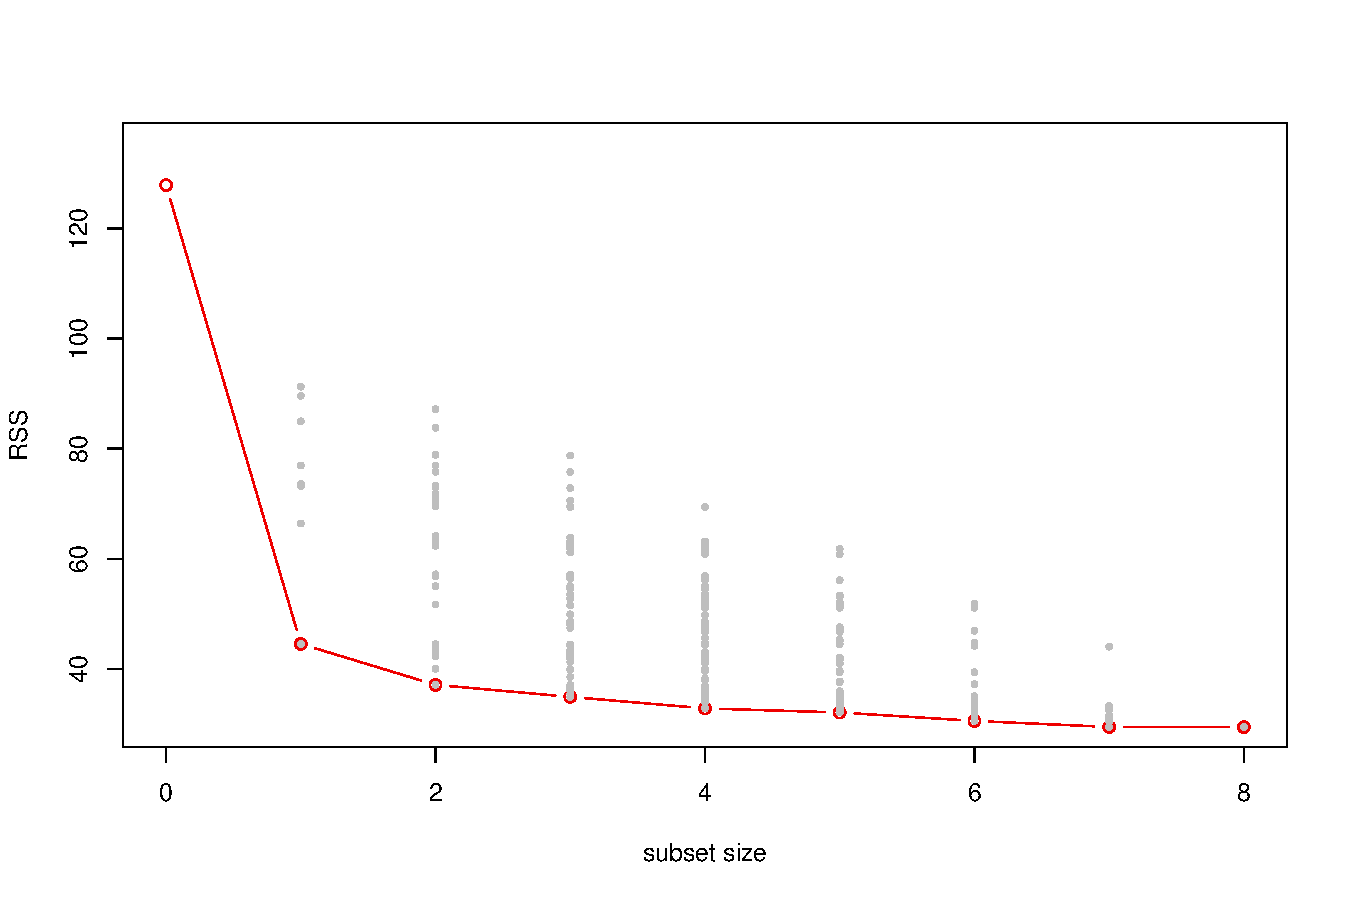
\includegraphics[width=\textwidth]{figures/subsetunnamed-chunk-26-1} 

\end{knitrout}
\end{frame}

\begin{frame}
  \frametitle{Recherche exhaustive III}
\begin{knitrout}\scriptsize
\definecolor{shadecolor}{rgb}{0.969, 0.969, 0.969}\color{fgcolor}
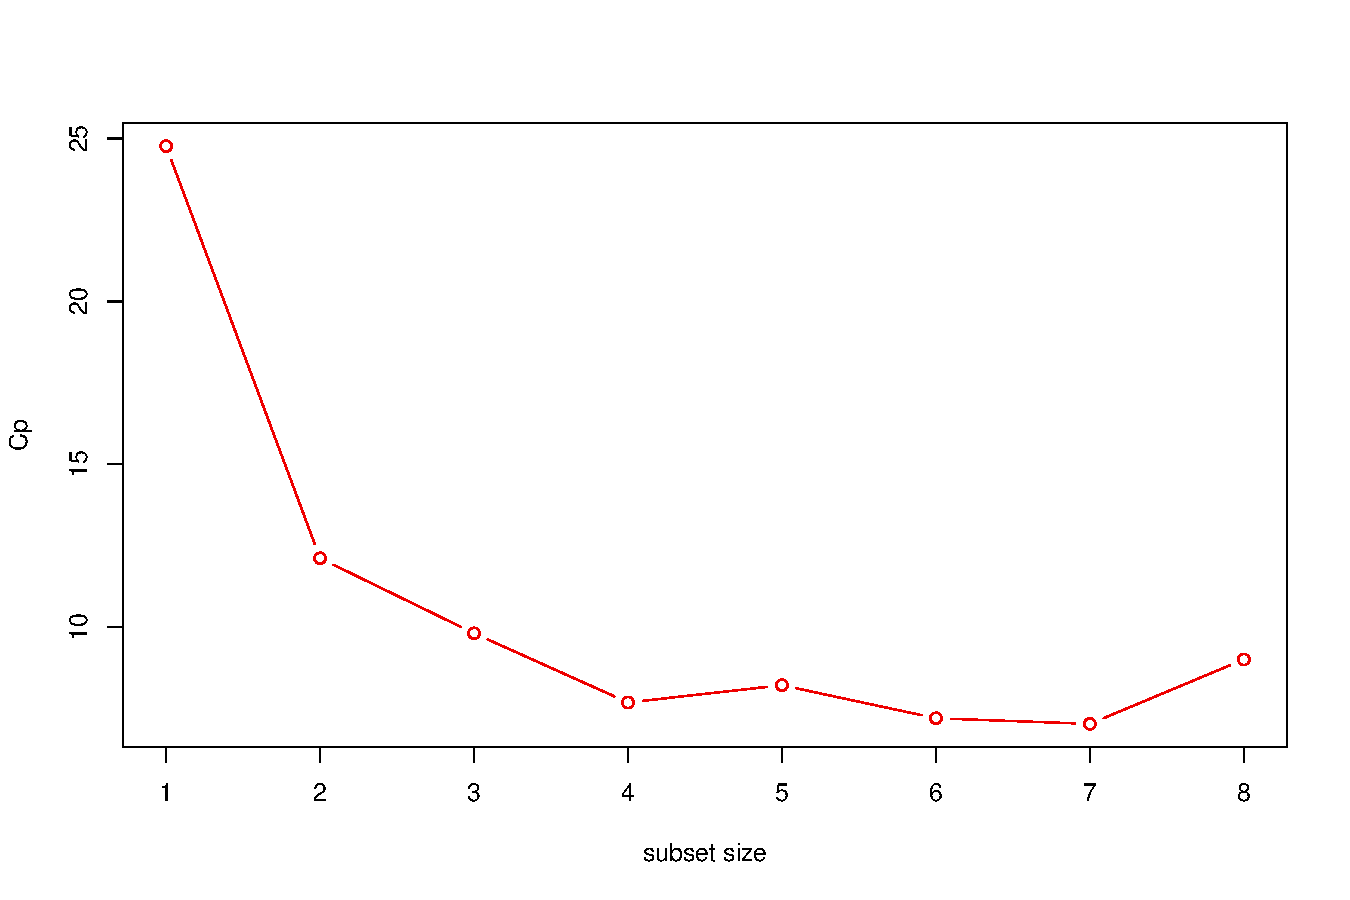
\includegraphics[width=\textwidth]{figures/subsetunnamed-chunk-27-1} 

\end{knitrout}
\end{frame}

\begin{frame}
  \frametitle{Recherche exhaustive VI}

\begin{knitrout}\scriptsize
\definecolor{shadecolor}{rgb}{0.969, 0.969, 0.969}\color{fgcolor}
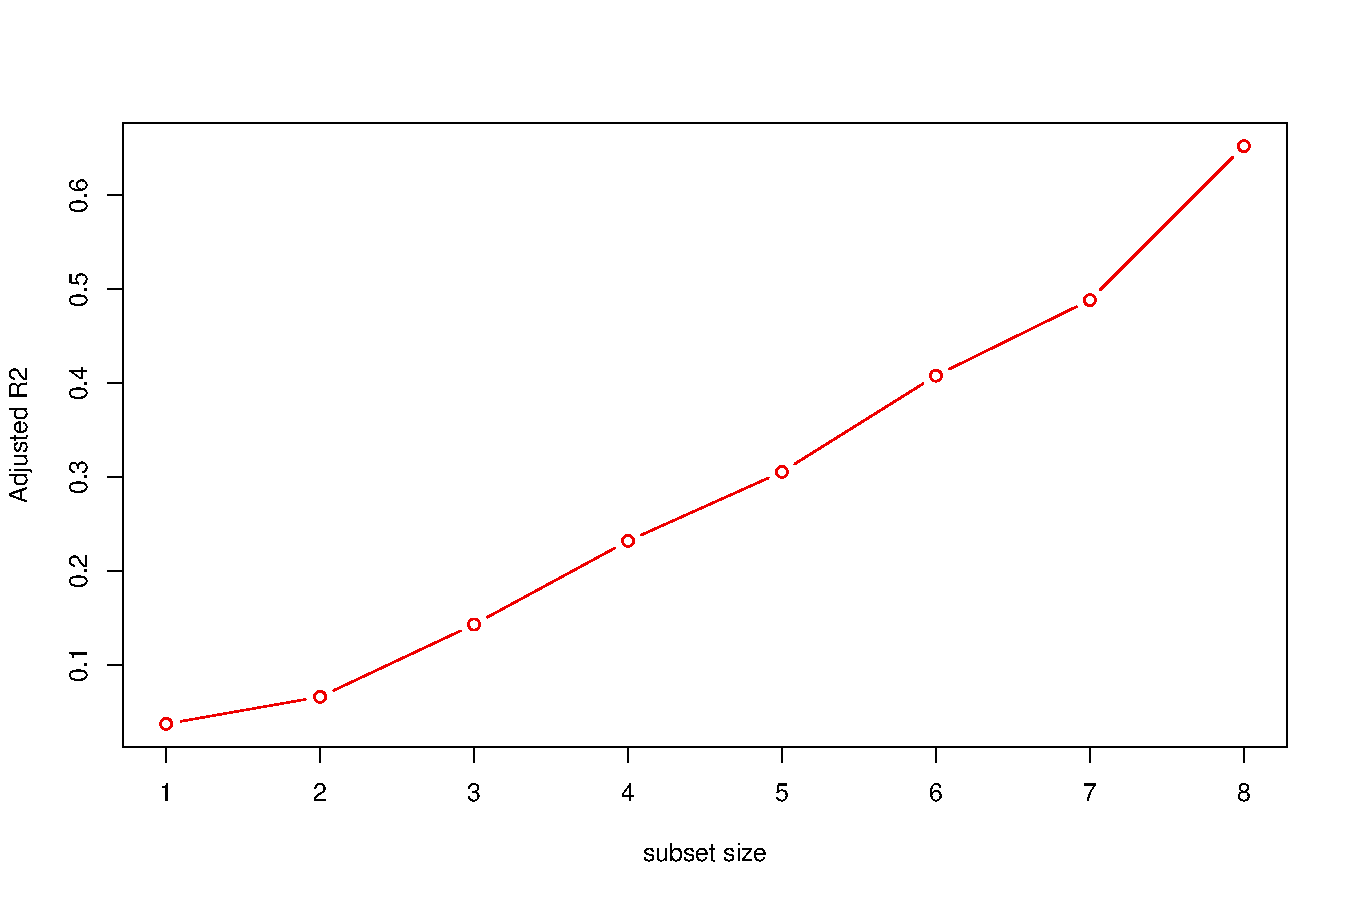
\includegraphics[width=\textwidth]{figures/subsetunnamed-chunk-28-1} 

\end{knitrout}

\end{frame}

\begin{frame}
  \frametitle{Recherche exhaustive V}

\begin{knitrout}\scriptsize
\definecolor{shadecolor}{rgb}{0.969, 0.969, 0.969}\color{fgcolor}
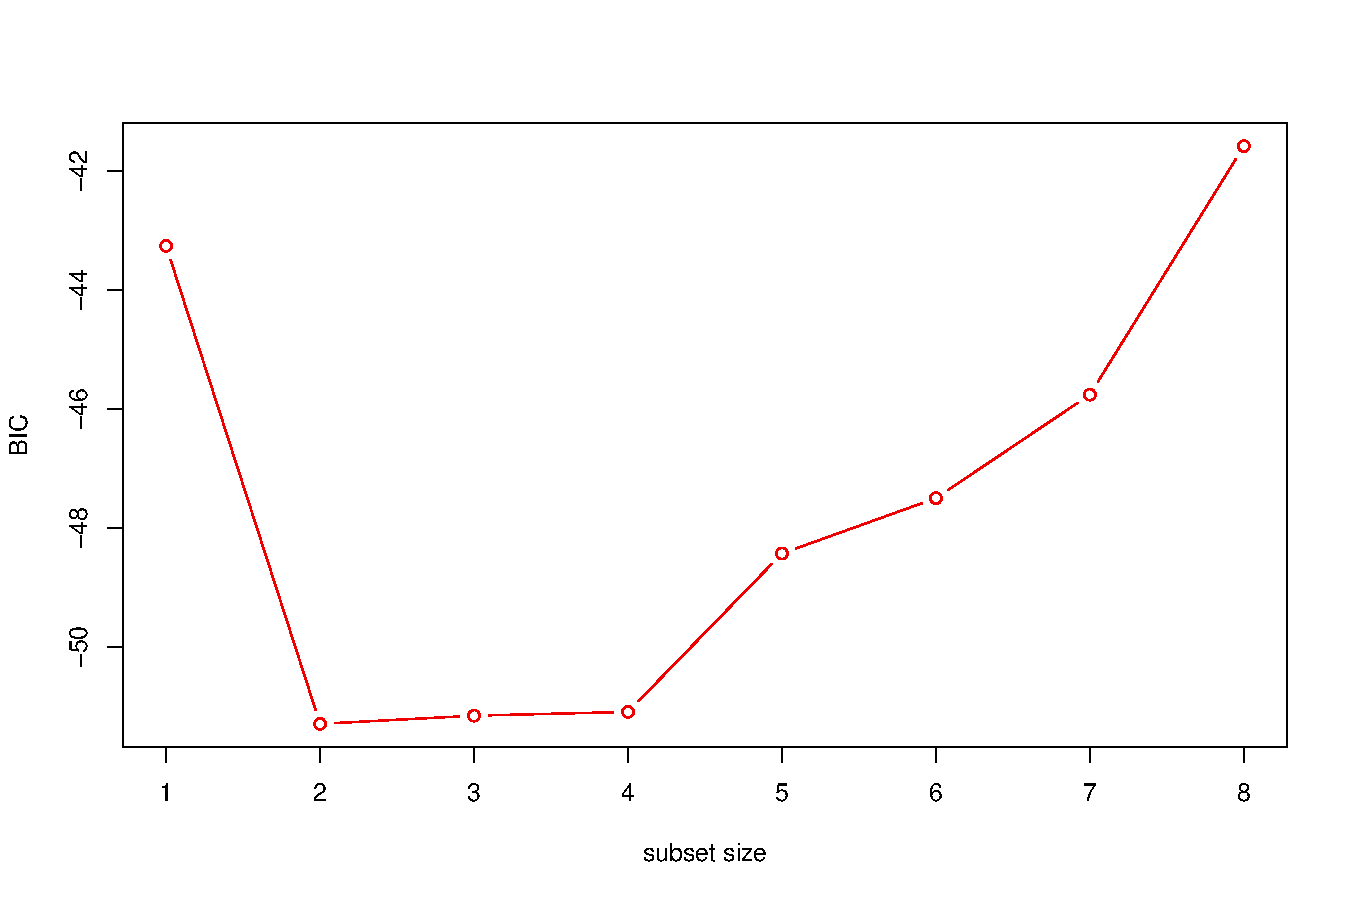
\includegraphics[width=\textwidth]{figures/subsetunnamed-chunk-29-1} 

\end{knitrout}

\end{frame}

\begin{frame}[containsverbatim]
  \frametitle{Forward-Stepwise dans \texttt{R} (I)}

Création du modèle nul et du modèle plein
\begin{knitrout}\scriptsize
\definecolor{shadecolor}{rgb}{0.969, 0.969, 0.969}\color{fgcolor}\begin{kframe}
\begin{alltt}
\hlstd{null}  \hlkwb{<-} \hlkwd{lm}\hlstd{(lpsa} \hlopt{~} \hlnum{1}\hlstd{,} \hlkwc{data}\hlstd{=prostate.train)}
\hlstd{full}  \hlkwb{<-} \hlkwd{lm}\hlstd{(lpsa} \hlopt{~} \hlstd{.,} \hlkwc{data}\hlstd{=prostate.train)}
\end{alltt}
\end{kframe}
\end{knitrout}

Création de l'ensemble des modèles à parcourir (\og scope\fg)
\begin{knitrout}\scriptsize
\definecolor{shadecolor}{rgb}{0.969, 0.969, 0.969}\color{fgcolor}\begin{kframe}
\begin{alltt}
\hlstd{lower} \hlkwb{<-} \hlopt{~}\hlnum{1}
\hlstd{upper} \hlkwb{<-} \hlopt{~}\hlstd{lcavol}\hlopt{+}\hlstd{lweight}\hlopt{+}\hlstd{age}\hlopt{+}\hlstd{lbph}\hlopt{+}\hlstd{svi}\hlopt{+}\hlstd{lcp}\hlopt{+}\hlstd{gleason}\hlopt{+}\hlstd{pgg45}
\hlstd{scope} \hlkwb{<-} \hlkwd{list}\hlstd{(}\hlkwc{lower}\hlstd{=lower,}\hlkwc{upper}\hlstd{=upper)}
\end{alltt}
\end{kframe}
\end{knitrout}

Stepwise avec AIC: forward, backward, both
\begin{knitrout}\scriptsize
\definecolor{shadecolor}{rgb}{0.969, 0.969, 0.969}\color{fgcolor}\begin{kframe}
\begin{alltt}
\hlstd{fwd}  \hlkwb{<-} \hlkwd{step}\hlstd{(null, scope,} \hlkwc{direction}\hlstd{=}\hlstr{"forward"} \hlstd{,} \hlkwc{trace}\hlstd{=}\hlnum{FALSE}\hlstd{)}
\hlstd{bwd}  \hlkwb{<-} \hlkwd{step}\hlstd{(full, scope,} \hlkwc{direction}\hlstd{=}\hlstr{"backward"}\hlstd{,} \hlkwc{trace}\hlstd{=}\hlnum{FALSE}\hlstd{)}
\hlstd{both} \hlkwb{<-} \hlkwd{step}\hlstd{(null, scope,} \hlkwc{direction}\hlstd{=}\hlstr{"both"}   \hlstd{,} \hlkwc{trace}\hlstd{=}\hlnum{FALSE}\hlstd{)}
\end{alltt}
\end{kframe}
\end{knitrout}

\vfill

$\rightsquigarrow$ 3  modèles équivalents
\end{frame}

\begin{frame}[containsverbatim]
  \frametitle{Forward regression}

\begin{scriptsize}
\begin{knitrout}\scriptsize
\definecolor{shadecolor}{rgb}{0.969, 0.969, 0.969}\color{fgcolor}\begin{kframe}
\begin{alltt}
\hlstd{fwd}
\end{alltt}
\begin{verbatim}
## 
## Call:
## lm(formula = lpsa ~ lcavol + lweight + svi + lbph, data = prostate.train)
## 
## Coefficients:
## (Intercept)       lcavol      lweight          svi         lbph  
##     -0.3259       0.9177       1.9853       0.3203       0.2052
\end{verbatim}
\begin{alltt}
\hlstd{fwd}\hlopt{$}\hlstd{anova}
\end{alltt}
\begin{verbatim}
##        Step Df  Deviance Resid. Df Resid. Dev       AIC
## 1           NA        NA        66   96.28145  26.29306
## 2  + lcavol -1 51.752862        65   44.52858 -23.37361
## 3 + lweight -1  7.436737        64   37.09185 -33.61680
## 4     + svi -1  2.184097        63   34.90775 -35.68291
## 5    + lbph -1  2.092754        62   32.81499 -37.82507
\end{verbatim}
\end{kframe}
\end{knitrout}
\end{scriptsize}
  
\end{frame}

\begin{frame}[containsverbatim]
  \frametitle{Backward regression}

\begin{scriptsize}
\begin{knitrout}\scriptsize
\definecolor{shadecolor}{rgb}{0.969, 0.969, 0.969}\color{fgcolor}\begin{kframe}
\begin{alltt}
\hlstd{bwd}
\end{alltt}
\begin{verbatim}
## 
## Call:
## lm(formula = lpsa ~ lcavol + lweight + age + lbph + svi + lcp + 
##     pgg45, data = prostate.train)
## 
## Coefficients:
## (Intercept)       lcavol      lweight          age         lbph  
##      0.2591       1.0419       2.2814      -1.2791       0.2116  
##         svi          lcp        pgg45  
##      0.3536      -0.2911       0.3532
\end{verbatim}
\begin{alltt}
\hlstd{bwd}\hlopt{$}\hlstd{anova}
\end{alltt}
\begin{verbatim}
##        Step Df   Deviance Resid. Df Resid. Dev       AIC
## 1           NA         NA        58   29.42638 -37.12766
## 2 - gleason  1 0.01091586        59   29.43730 -39.10281
\end{verbatim}
\end{kframe}
\end{knitrout}
\end{scriptsize}

\end{frame}
\begin{frame}[containsverbatim]
  \frametitle{Stepwise regression}

\begin{scriptsize}
\begin{knitrout}\scriptsize
\definecolor{shadecolor}{rgb}{0.969, 0.969, 0.969}\color{fgcolor}\begin{kframe}
\begin{alltt}
\hlstd{both}
\end{alltt}
\begin{verbatim}
## 
## Call:
## lm(formula = lpsa ~ lcavol + lweight + svi + lbph, data = prostate.train)
## 
## Coefficients:
## (Intercept)       lcavol      lweight          svi         lbph  
##     -0.3259       0.9177       1.9853       0.3203       0.2052
\end{verbatim}
\begin{alltt}
\hlstd{both}\hlopt{$}\hlstd{anova}
\end{alltt}
\begin{verbatim}
##        Step Df  Deviance Resid. Df Resid. Dev       AIC
## 1           NA        NA        66   96.28145  26.29306
## 2  + lcavol -1 51.752862        65   44.52858 -23.37361
## 3 + lweight -1  7.436737        64   37.09185 -33.61680
## 4     + svi -1  2.184097        63   34.90775 -35.68291
## 5    + lbph -1  2.092754        62   32.81499 -37.82507
\end{verbatim}
\end{kframe}
\end{knitrout}
\end{scriptsize}
  
\end{frame}

\begin{frame}[containsverbatim]
  \frametitle{Évaluation sur données test}

\begin{knitrout}\scriptsize
\definecolor{shadecolor}{rgb}{0.969, 0.969, 0.969}\color{fgcolor}\begin{kframe}
\begin{alltt}
\hlkwd{print}\hlstd{(err.ols)}
\end{alltt}
\begin{verbatim}
## [1] 0.5221043
\end{verbatim}
\begin{alltt}
\hlkwd{print}\hlstd{(err.AIC.fwd}  \hlkwb{<-} \hlkwd{mean}\hlstd{((y.test}\hlopt{-}\hlkwd{predict}\hlstd{(fwd ,prostate.test))}\hlopt{^}\hlnum{2}\hlstd{))}
\end{alltt}
\begin{verbatim}
## [1] 0.4520967
\end{verbatim}
\begin{alltt}
\hlkwd{print}\hlstd{(err.AIC.bwd}  \hlkwb{<-} \hlkwd{mean}\hlstd{((y.test}\hlopt{-}\hlkwd{predict}\hlstd{(bwd ,prostate.test))}\hlopt{^}\hlnum{2}\hlstd{))}
\end{alltt}
\begin{verbatim}
## [1] 0.517824
\end{verbatim}
\begin{alltt}
\hlkwd{print}\hlstd{(err.AIC} \hlkwb{<-} \hlkwd{mean}\hlstd{((y.test}\hlopt{-}\hlkwd{predict}\hlstd{(both,prostate.test))}\hlopt{^}\hlnum{2}\hlstd{))}
\end{alltt}
\begin{verbatim}
## [1] 0.4520967
\end{verbatim}
\end{kframe}
\end{knitrout}
\end{frame}


\begin{frame}[containsverbatim]
  \frametitle{Stepwise en  \texttt{R}: modification pour le BIC}
  \framesubtitle{Modèle plus parcimonieux}
  
\begin{knitrout}\scriptsize
\definecolor{shadecolor}{rgb}{0.969, 0.969, 0.969}\color{fgcolor}\begin{kframe}
\begin{alltt}
\hlstd{BIC} \hlkwb{<-} \hlkwd{step}\hlstd{(null, scope,} \hlkwc{k}\hlstd{=}\hlkwd{log}\hlstd{(n} \hlkwb{<-} \hlkwd{nrow}\hlstd{(prostate)),} \hlkwc{trace}\hlstd{=}\hlnum{FALSE}\hlstd{)}
\hlstd{BIC}
\end{alltt}
\begin{verbatim}
## 
## Call:
## lm(formula = lpsa ~ lcavol + lweight, data = prostate.train)
## 
## Coefficients:
## (Intercept)       lcavol      lweight  
##      -1.049        1.139        2.720
\end{verbatim}
\begin{alltt}
\hlkwd{print}\hlstd{(err.BIC}  \hlkwb{<-} \hlkwd{mean}\hlstd{((y.test}\hlopt{-}\hlkwd{predict}\hlstd{(BIC ,prostate.test))}\hlopt{^}\hlnum{2}\hlstd{))}
\end{alltt}
\begin{verbatim}
## [1] 0.4908699
\end{verbatim}
\end{kframe}
\end{knitrout}
\end{frame}


\begin{frame}
  \frametitle{Sélection variable : quelques remarques}

  \begin{block}{Interprétabilité}
    \begin{enumerate}
    \item Si  le vrai $\mathcal{S}$ ne contient que \alert{\bf quelques
      variables liées à la  response},\\
      $\rightsquigarrow$ les algorithmes de  sélection  peuvent  retrouver  les  prédicteurs pertinents.
    \item  Si  le vrai   $\mathcal{S}$  contient \alert{\bf beaucoup  de
      variables  très corrélées}\\
      $\rightsquigarrow$  les  variables sélectionnées  seront difficiles à interpréter.
    \end{enumerate}
  \end{block}

  \vfill

  \begin{block}{Limites liées à la stabilité}
    En présence de prédicteurs très corrélés ou lorsque $n < p$, \alert{\bf de  petites perturbations} des
   données  peuvent  provoquer  de \alert{\bf grandes  différences}  entre  les
    ensembles de variables sélectionnées.
   \end{block}
  
\end{frame}

\section{Régularisation}


\subsection{Motivations et principe}

\begin{frame}
  \frametitle{Objectifs}

  Contrôler le vecteur $\hatbbeta$ pour

  \begin{enumerate}
  \item \alert{Régulariser} le problème
    \begin{itemize}
    \item Pour des questions numériques, (conditionnement de $\bX^T\bX$),
    \item Pour des questions de stabilité, (corrélations entre les $(X_1,\dots,X_p)$).
    \end{itemize}
    \bigskip
  \item \alert{Améliorer} la prédiction
    \begin{itemize}
    \item En augmentant le biais pour diminuer la variance
    \item En contrôlant les variables non pertinentes
    \end{itemize}
    \bigskip
  \item \alert{Favoriser} l'interprétabilité
    \begin{itemize}
    \item En contrôlant la complexité du modèle,
    \item En intégrant la sélection de variable (Lasso).
    \end{itemize}
  \end{enumerate}

\end{frame}

\pgfdeclareimage[height=0.8\textheight]{sparsity1}{figures/sparsity_1}
\pgfdeclareimage[height=0.8\textheight]{sparsity2}{figures/sparsity_2}
\pgfdeclareimage[height=0.375\textheight]{sparsity4}{figures/sparsity_4}

%--------------------------------------%

\begin{frame}
  \frametitle{Une vue géométrique de la régularisation}
  \framesubtitle{Optimisation sous contraintes}

  \begin{overlayarea}{\textwidth}{\textheight}
    \begin{columns}
      \begin{column}{0.475\textwidth}
        \begin{tikzpicture}
          \only<1>{%
            \node (Surf) at (0,0) {\pgfuseimage{sparsity1}}
            node     at    (Surf.west)    [rotate=90,yshift=5mm]
            {$L(\beta_1,\beta_2;\mathbf{X})$}
            node at (Surf.south west) [xshift=5mm,yshift=5mm]{$\beta_2$}
            node at (Surf.south east) [xshift=-7.5mm,yshift=2.5mm]{$\beta_1$};
          }
          \only<2>{%
            \node (Surf2) at (0,0) {\pgfuseimage{sparsity2}}
            node    at    (Surf2.west)    [rotate=90,yshift=5mm]
            {$L(\beta_1,\beta_2;\mathbf{X})$}
            node at (Surf2.south west) [xshift=5mm,yshift=5mm]{$\beta_2$}
            node at (Surf2.south east) [xshift=-7.5mm,yshift=2.5mm]{$\beta_1$};
          }
          \only<3->{%
            \node (titi) at (0,0) {\phantom{titi}};
            \node (Surf3) at (0,-4.5) {\pgfuseimage{sparsity4}}
            node at (Surf3.west) [rotate=90,yshift=2.5mm] {$\beta_2$}
            node at (Surf3.south) [yshift=-2.5mm] {$\beta_1$};
          }
        \end{tikzpicture}
      \end{column}
      \begin{column}{0.55\textwidth}
        \only<1>{%
          On veut résoudre un problème de la forme
          \begin{equation*}
            \maximize_{\beta_1,\beta_2} L(\beta_1,\beta_2;\mathbf{X})
          \end{equation*}
          où $L$ est typiquement une vraisemblance concave, ce qui est équivalent à 
          \begin{equation*}
            \minimize_{\beta_1,\beta_2} L'(\beta_1,\beta_2;\mathbf{X})
          \end{equation*}
          où $L'=-L$ est convexe (par exemple, la perte de l'OLS).
        }
        \only<2->{%
          On restreint l'espace des $\bbeta$, ainsi
          \begin{equation*}
            \left\{\begin{array}{ll}
                \displaystyle    \maximize_{\beta_1,\beta_2}   &
                L(\beta_1,\beta_2;\mathbf{X})\\
                \mathrm{s.t.} & \Omega(\beta_1,\beta_2) \leq c
              \end{array}\right.,
          \end{equation*}
          où $\Omega$ définit un ensemble de \textit{constraintes} sur
          $\boldsymbol\beta$.
        }
        \only<3->{%
          \begin{equation*}
            \Updownarrow
          \end{equation*}
          \begin{equation*}
            \minimize_{\beta_1,\beta_2} J(\bbeta),
          \end{equation*}
          où $J$ est la fonction objectif (convexe) définie par
          \begin{equation*}
            J(\bbeta) = - L(\beta_1,\beta_2;\mathbf{X}) + \lambda \Omega(\beta_1,\beta_2)
          \end{equation*}
        }

        \only<4>{
          \begin{center}
            Comment choisir $\Omega$ ?
          \end{center}
        }
      \end{column}
    \end{columns}
  \end{overlayarea}
\end{frame}




\subsection{La régression Ridge}

\subsubsection{Définition de l'estimateur}

\begin{frame}
  \frametitle{Définition}

  \begin{block}{Remarque}
    Si les   $\beta_j$ ne sont pas contraints,  ils peuvent prendre de très grandes valeurs et donc avoir une grande variance.
  \end{block}

  \begin{block}{Idée}
    Pour contrôler la variance, il faut contrôler la taille des coefficients de  $\bbeta$. Cette approche pourrait réduire sensiblement l'erreur de prédiction.
  \end{block}

  \onslide<2>{
  \begin{overlayarea}{\textwidth}{.4\textheight}
    \begin{columns}
      \begin{column}[c]{.6\textwidth}
        \begin{block}{La Ridge comme problème de régularisation}
          \begin{equation*}
            \hat{\bbeta}^{\text{ridge}}     =    \argmin_{\bbeta\in\Rset^{p+1}}
            \mathrm{RSS}(\bbeta), \quad  \text{s.c. } \sum_{j=1}^p \beta_j^2
            \leq s,
          \end{equation*}
          où $s$ est un facteur de rétrécissement.
        \end{block}
      \end{column}
      \begin{column}{.4\textwidth}
         \includegraphics<2>{figures/ridge_set}
      \end{column}
    \end{columns}
  \end{overlayarea}
  }
\end{frame}

\begin{frame}
  \frametitle{Un exemple en deux dimensions}

  Considérons que le vrai modèle est  $Y = X_1 \beta_1 + X_2\beta_2
  +  \varepsilon$. Si $X_1$ et   $X_2$ sont très corrélés, alors
  $X_1\approx X_2$. De plus pour tout $\gamma\geq 0$,
  \begin{align*}
    Y & = X_1 (\beta_1 + \gamma) + X_2 (\beta_2 - \gamma) +
    \gamma(X_1-X_2) + \varepsilon \\
    & \approx X_1 (\beta_1 + \gamma) + X_2 (\beta_2 - \gamma) + \varepsilon.
  \end{align*}
  On prédit une réponse similaire pour un large panel d'estimateur de  $\bbeta$ indexés sur  $\gamma$.

  \vfill

  \onslide<2->{
    Pour de petits $s$, la régression  Ridge contrôle
    \begin{equation*}
      (\beta_1 + \gamma)^2 + (\beta_2 - \gamma)^2
    \end{equation*}
    qui est minimale pour $\gamma =  (\beta_2-\beta_1)/2$, et dans ce cas $\beta_j = (\beta_1 + \beta_2)/2$.
  }

 \vfill

\onslide<3>{$\rightsquigarrow$ La Ridge \og moyenne \fg\ les coefficients associés aux prédicteurs corrélés.}

\end{frame}







\begin{frame}[containsverbatim,allowframebreaks]
  \frametitle{Un exemple en deux dimensions (en \texttt{R})}

On génère deux prédicteurs corrélés
\begin{knitrout}\scriptsize
\definecolor{shadecolor}{rgb}{0.969, 0.969, 0.969}\color{fgcolor}\begin{kframe}
\begin{alltt}
\hlkwd{suppressMessages}\hlstd{(}\hlkwd{library}\hlstd{(quadrupen))}
\hlstd{x1} \hlkwb{<-} \hlkwd{rnorm}\hlstd{(}\hlnum{5}\hlstd{)}
\hlstd{x2} \hlkwb{<-} \hlstd{x1} \hlopt{+} \hlkwd{rnorm}\hlstd{(}\hlnum{5}\hlstd{,}\hlnum{0}\hlstd{,} \hlnum{0.5}\hlstd{)}
\hlkwd{cor}\hlstd{(x1,x2)}
\end{alltt}
\begin{verbatim}
## [1] 0.7188671
\end{verbatim}
\end{kframe}
\end{knitrout}

On génère $Y$ et on trace le \alert{\bf chemin de régularisation}
\begin{knitrout}\scriptsize
\definecolor{shadecolor}{rgb}{0.969, 0.969, 0.969}\color{fgcolor}\begin{kframe}
\begin{alltt}
\hlstd{y} \hlkwb{<-} \hlstd{x1} \hlopt{+} \hlstd{x2} \hlopt{+}\hlkwd{rnorm}\hlstd{(}\hlnum{5}\hlstd{)}
\hlkwd{plot}\hlstd{(}\hlkwd{ridge}\hlstd{(}\hlkwd{cbind}\hlstd{(x1,x2),y))}
\end{alltt}
\end{kframe}
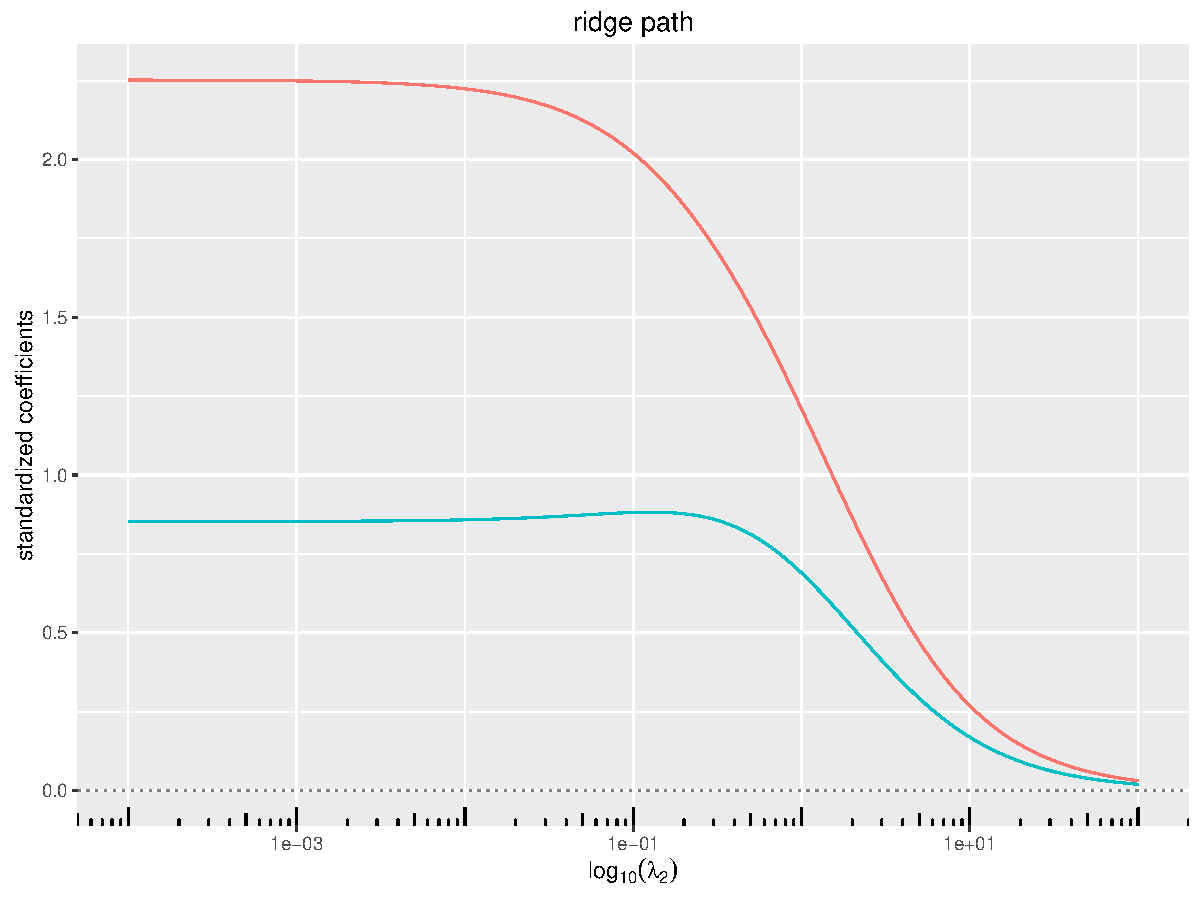
\includegraphics[width=\textwidth]{figures/toy_ridgeunnamed-chunk-43-1} 

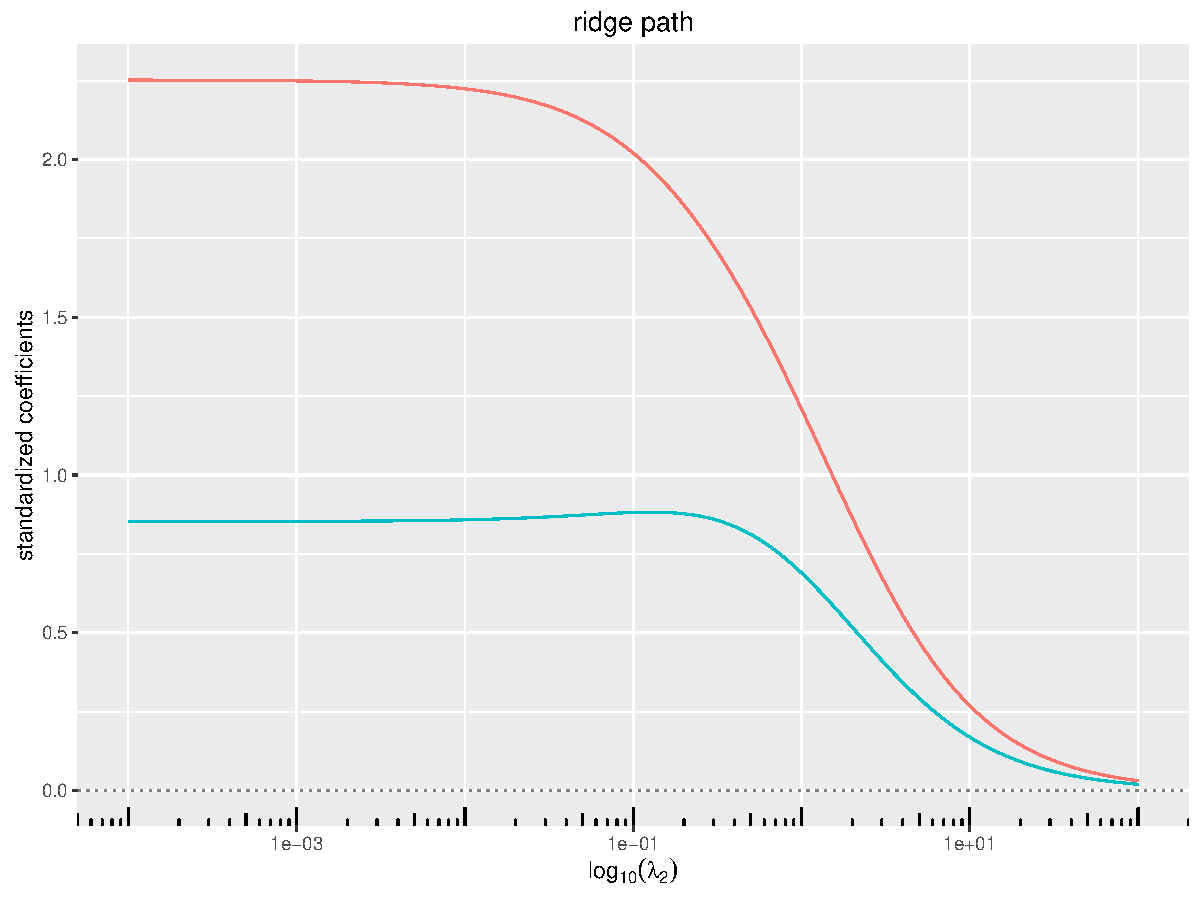
\includegraphics[width=\textwidth]{figures/toy_ridgeunnamed-chunk-43-2} 

\end{knitrout}

\end{frame}

\begin{frame}
  \frametitle{La ridge comme un problème de régression pénalisée}

  \alert{On ne pénalise pas la constante} et on considère donc  $\bbeta  =
  (\beta_1,\dots\beta_p)$ et on pose
  \begin{itemize}
  \item $\hatbeta_0 = \bar{\by} - \bar{x}\hatbbeta$
  \item on centre $\mathbf{y}$ et $\mathbf{x}_j$, $j=1,\dots,p$.
  \end{itemize}
  \alert{On normalise $\bx_j$} pour ajuster et on renvoie les estimations
  $\hatbbetaridge$ dans l'\alert{échelle d'origine}.

  \vfill

  \begin{block}{Forme Lagrangienne (convexe)}
    \vspace{-.5cm}
    \begin{align*}
      \hat{\bbeta}^{\text{ridge}} &  =   \argmin_{\bbeta\in\R^p}  \frac{1}{2}
      \|\mathbf{y} - \mathbf{X} \bbeta\|^2 + \lambda \|\bbeta\|^2\\
      & = (\mathbf{X}^\intercal \mathbf{X} +
      \lambda \mathbf{I}_p)^{-1} \mathbf{X}^\intercal \mathbf{y} = \mathbf{H}_\lambda \by.
    \end{align*}
  \end{block}

  \vfill

  \begin{block}{Forte convexité}
    Contrairement à l'OLS, une solution unique existe toujours quand    $\lambda>0$ quelque soit le conditionnement de la matrice
    $\mathbf{X}^\intercal \mathbf{X}$.
  \end{block}

\end{frame}

\subsubsection{Propriétés et résolution pratique}

\begin{frame}
  \frametitle{Connexion à l'OLS}

  Soit $\mathbf{S}_\lambda =  \mathbf{X}^\intercal \mathbf{X} + \lambda
  \mathbf{I}_p$.  Alors
  \begin{equation*}
    \hat{\bbeta}^{\text{ridge}} =
    \mathbf{S}_\lambda^{-1}        \mathbf{X}^\intercal       \mathbf{X}
    \hat{\bbeta}^{\text{ols}} =
    \left(\mathbf{I}_p - \lambda\mathbf{S}_\lambda^{-1}\right) \hat{\bbeta}^{\text{ols}}.
  \end{equation*}
  Lorsque       $\lambda=0$,       $\hat{\bbeta}^{\text{ridge}}$      et
  $\hat{\bbeta}^{\text{ols}}$ coincident.

  \begin{columns}
    \begin{column}[c]{.5\textwidth}
      Dans le cas d'un design orthonormal, $\mathbf{X}^\intercal
      \mathbf{X}=\mathbf{I}$ et
      \begin{equation*}
        \hat{\bbeta}^{\text{ridge}} = \frac{1}{1+\lambda} \hat{\bbeta}^{\text{ols}}.
      \end{equation*}
    \end{column}

    \begin{column}[c]{.5\textwidth}
      \begin{center}
        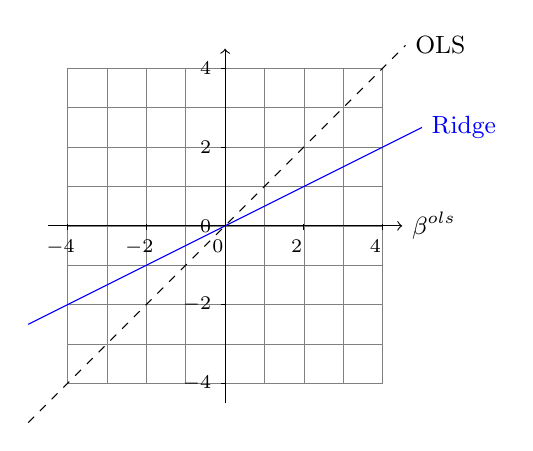
\begin{tikzpicture}[scale=.5,font=\small]
          \draw[very thin,color=gray] (-4,-4) grid [xstep=1,ystep=1] (4,4);
          \draw[->] (-4.5,0) -- (4.5,0) node[right] {$\beta^{\text{ols}}$};
          \draw[->] (0,-4.5) -- (0,4.5) ;
          \draw[color=blue] plot[samples=200] (\x,{1/(2)*\x})
          node[right] {Ridge};
          \draw[dashed,color=black] plot (\x,{\x}) node[right] {OLS};

          % units for cartesian reference frame
          \foreach \x in {-4,-2,0,2,4}{
            \draw (\x cm,1pt)  -- (\x cm,-3pt)
            node[anchor=north,xshift=-0.09cm] {\scriptsize$\x$};
            \draw (1pt,\x cm) -- (-3pt,\x cm)
            node[anchor=east] {\scriptsize$\x$};
          }
        \end{tikzpicture}
      \end{center}
    \end{column}
  \end{columns}

\end{frame}

\begin{frame}
  \frametitle{Biais et variance de l'estimateur Ridge}

  \begin{proposition}
    \begin{equation*}
      \E\left(\hat{\bbeta}^{\text{ridge}}-\hatbbetaols\right)   =
      -\lambda \mathbf{S}_\lambda^{-1} \bbeta,       \var\left(\hat{\bbeta}^{\text{ridge}}\right)  =
      \sigma^2 \mathbf{S}_\lambda^{-1} \mathbf{X}^\intercal \mathbf{X}
      \mathbf{S}_\lambda^{-1}.
    \end{equation*}
    et
    \begin{equation*}
      \var(\hatbbetaols) - \var(\hatbbetaridge) \succeq 0
    \end{equation*}
    donc
    $\var(x^T\hatbbetaols) \geq \var(x^T\hatbbetaridge)$ un $x$ fixé.
  \end{proposition}

  \vfill

  \begin{itemize}
  \item quand $\lambda\to 0$, sans biais, grande variance (OLS)
  \item quand $\lambda\to \infty$, grand biais, variance nulle.
  \end{itemize}

  \vfill

  $\rightsquigarrow$  Un compromis  est nécessaire  (\textit{i.e.}, un bon choix pour $\lambda$).

\end{frame}

\begin{frame}
  \frametitle{Calcul pratique du chemin de solution}
  \framesubtitle{Ridge et SVD}

  \begin{block}{Décomposition en valeur singulière --
      \href{{http://upload.wikimedia.org/wikipedia/commons/e/e9/Singular_value_decomposition.gif}}{lien
        vers une illustration}}
    \begin{equation*}
      \mathbf{X} = \mathbf{U} \mathbf{D} \mathbf{V}^\intercal,
    \end{equation*}
    \vspace{-.5cm}
    \begin{itemize}
    \item  $\mathbf{U}$  est  une   matrice  $n\times  min(n,p)$  orthogonale
      génératrice de l'espace ligne,
    \item  $\mathbf{V}$  est  une   matrice  $p\times  min(n,p)$  orthogonale
      génératice de l'espace colonne,
    \item     $\mathbf{D}=     \mathrm{diag}(d_1,\dots,d_i,\dots,d_min(n,p))$
      contient les valeurs singulières de $\mathbf{X}$.
    \end{itemize}
  \end{block}

  \vfill

  \begin{equation*}
    \hat{\bbeta}^{\mathrm{ridge}}      =      \mathbf{V}
    {\boldsymbol\Delta}_\lambda \mathbf{U}^\intercal \mathbf{y},
  \end{equation*}
  où ${\boldsymbol\Delta}_\lambda$ est une matrice diagonale telle que
  $\Delta_i= d_i/(d_i^2+\lambda)$.

  \vfill

  \begin{block}{Coût algorithmique}
    Le calcul du chemin de solution complet pour $K$ valeurs de $\lambda$ nécessite
    \begin{enumerate}
    \item une SVD ($\mathcal{O}(np^2)$)
    \item un produit matriciel entre $\mathbf{V}$ et la matrice $p\times K$
          ${\boldsymbol\Delta}_\lambda     \mathbf{U}^\intercal
      \mathbf{y}$
    \end{enumerate}
  \end{block}
\end{frame}

\begin{frame}
  \frametitle{Interprétation liée à la SVD}

  \begin{block}{Pour les moindres carrés}
    \begin{equation*}
      \mathbf{X}\hat{\bbeta}^{\text{ols}}                               =
      \mathbf{X}(\mathbf{X}^\intercal\mathbf{X})^{-1}          \mathbf{X}^\intercal
      \mathbf{y} = \mathbf{U} \mathbf{U}^\intercal \mathbf{y}.
    \end{equation*}
    où $\mathbf{U}^\intercal \mathbf{y}$ sont les coordonnées de 
    $\mathbf{y}$ dans la base orthornormale $\mathbf{U}$.
  \end{block}

  \vfill

  \begin{block}{Pour la ridge}
    \begin{equation*}
      \mathbf{X}\hat{\bbeta}^{\text{ridge}}                               =
      \mathbf{X}(\mathbf{X}^\intercal\mathbf{X}                         +
      \lambda\mathbf{I}_p)^{-1} \mathbf{X}^\intercal
      \mathbf{y} = \sum_{j=1}^p \mathbf{u}_j \alert{\frac{d^2_j}{d^2_j+\lambda}}
      \mathbf{u}_j^\intercal \mathbf{y}.
    \end{equation*}
  \end{block}

  $\rightsquigarrow$ La régularisation ridge régularise plus les coefficients associées aux axes de faibles variance  $d_j$.

\end{frame}


\begin{frame}[containsverbatim]
  \frametitle{Une implémentation \texttt{R} possible pour la régression Ridge}

  \begin{tiny}
\begin{knitrout}\scriptsize
\definecolor{shadecolor}{rgb}{0.969, 0.969, 0.969}\color{fgcolor}\begin{kframe}
\begin{alltt}
\hlstd{ridge.regression} \hlkwb{<-} \hlkwa{function}\hlstd{(}\hlkwc{x}\hlstd{,}\hlkwc{y}\hlstd{,}\hlkwc{lambda}\hlstd{=}\hlnum{0}\hlstd{)\{}
  \hlcom{## x is assumed to be centered/scaled by the user}

  \hlstd{n.lambda} \hlkwb{<-} \hlkwd{length}\hlstd{(lambda)}
  \hlstd{variables} \hlkwb{<-} \hlkwd{colnames}\hlstd{(x)}
  \hlstd{p} \hlkwb{<-} \hlkwd{length}\hlstd{(variables)}

  \hlstd{SVD} \hlkwb{<-} \hlkwd{svd}\hlstd{(x)}
  \hlstd{d}  \hlkwb{<-} \hlkwd{rep}\hlstd{(SVD}\hlopt{$}\hlstd{d,n.lambda)}
  \hlstd{d2} \hlkwb{<-} \hlkwd{rep}\hlstd{(SVD}\hlopt{$}\hlstd{d}\hlopt{^}\hlnum{2}\hlstd{,n.lambda)}
  \hlstd{lambdas} \hlkwb{<-} \hlkwd{rep}\hlstd{(lambda,}\hlkwc{each}\hlstd{=p)}
  \hlstd{V} \hlkwb{<-} \hlstd{SVD}\hlopt{$}\hlstd{v}
  \hlstd{U} \hlkwb{<-} \hlstd{SVD}\hlopt{$}\hlstd{u}

  \hlstd{Delta} \hlkwb{<-} \hlstd{d}\hlopt{/}\hlstd{(d}\hlopt{^}\hlnum{2}\hlopt{+}\hlstd{lambdas)}
  \hlstd{beta}  \hlkwb{<-} \hlkwd{t}\hlstd{(V} \hlopt \hlkwd{matrix}\hlstd{((}\hlkwd{rep}\hlstd{(}\hlkwd{t}\hlstd{(U)} \hlopt \hlstd{y, n.lambda)} \hlopt{*} \hlstd{Delta),}\hlkwc{nrow}\hlstd{=p))}
  \hlstd{df}    \hlkwb{<-} \hlkwd{colSums}\hlstd{(}\hlkwd{matrix}\hlstd{(d2}\hlopt{/}\hlkwd{rep}\hlstd{(d2}\hlopt{+}\hlstd{lambdas,}\hlkwc{nrow}\hlstd{=p)))}
  \hlkwd{colnames}\hlstd{(beta)} \hlkwb{<-} \hlstd{variables}

  \hlkwd{return}\hlstd{(}\hlkwd{list}\hlstd{(}\hlkwc{beta}\hlstd{=beta,}\hlkwc{beta0}\hlstd{=}\hlkwd{mean}\hlstd{(y),}\hlkwc{df}\hlstd{=df))}
\hlstd{\}}
\end{alltt}
\end{kframe}
\end{knitrout}
\end{tiny}



\end{frame}

\begin{frame}[containsverbatim]
  \frametitle{Ridge et données du cancer de la prostate}

  \vfill

Calcul du chemin de solution
\begin{knitrout}\scriptsize
\definecolor{shadecolor}{rgb}{0.969, 0.969, 0.969}\color{fgcolor}\begin{kframe}
\begin{alltt}
\hlstd{ridge.path} \hlkwb{<-} \hlkwd{ridge}\hlstd{(x.train,y.train)}
\end{alltt}
\end{kframe}
\end{knitrout}

\vfill

Calcul de l'erreur de prédiction sur l'ensemble test pour tout $\lambda$
\begin{knitrout}\scriptsize
\definecolor{shadecolor}{rgb}{0.969, 0.969, 0.969}\color{fgcolor}\begin{kframe}
\begin{alltt}
\hlstd{err} \hlkwb{<-} \hlkwd{colMeans}\hlstd{((y.test}\hlopt{-}\hlkwd{predict}\hlstd{(ridge.path,x.test))}\hlopt{^}\hlnum{2}\hlstd{)}
\end{alltt}
\end{kframe}
\end{knitrout}

\vfill

Ainsi, le $\lambda^\star$ qui minimise cette erreur est 
\begin{knitrout}\scriptsize
\definecolor{shadecolor}{rgb}{0.969, 0.969, 0.969}\color{fgcolor}\begin{kframe}
\begin{alltt}
\hlstd{ridge.path}\hlopt{@}\hlkwc{lambda2}\hlstd{[}\hlkwd{which.min}\hlstd{(err)]}
\end{alltt}
\begin{verbatim}
## [1] 0.5722368
\end{verbatim}
\end{kframe}
\end{knitrout}

L'erreur de prédiction est légèrement meilleure que celle de l'OLS
\begin{knitrout}\scriptsize
\definecolor{shadecolor}{rgb}{0.969, 0.969, 0.969}\color{fgcolor}\begin{kframe}
\begin{alltt}
\hlstd{err.ridge} \hlkwb{<-} \hlstd{err[}\hlkwd{which.min}\hlstd{(err)]; err.ridge; err.ols}
\end{alltt}
\begin{verbatim}
##     0.572 
## 0.5148989
## [1] 0.5221043
\end{verbatim}
\end{kframe}
\end{knitrout}

\end{frame}

\begin{frame}[containsverbatim]
  \frametitle{Ridge et données du cancer de la prostate}
\begin{knitrout}\scriptsize
\definecolor{shadecolor}{rgb}{0.969, 0.969, 0.969}\color{fgcolor}
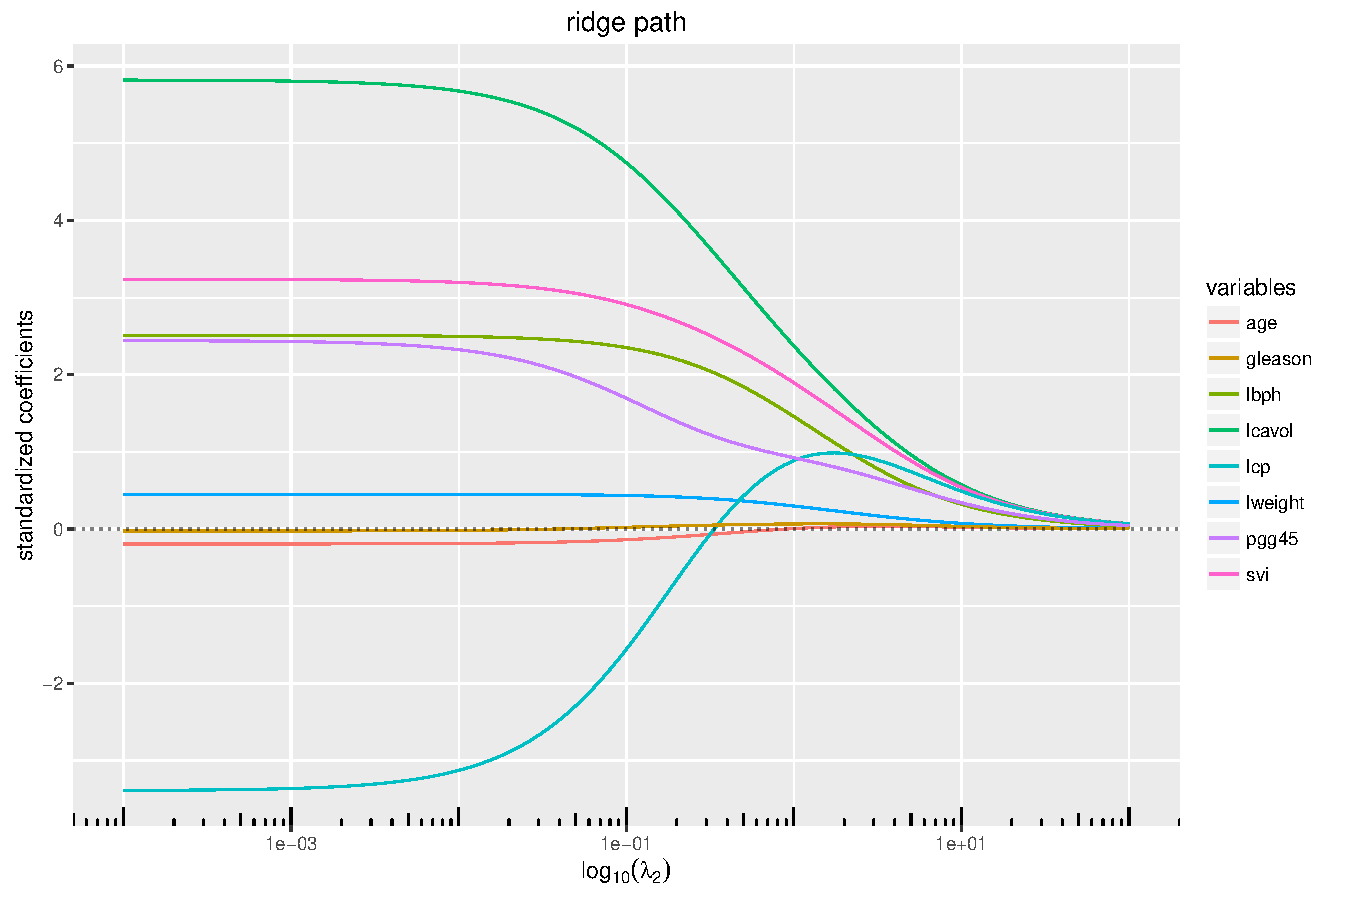
\includegraphics[width=\textwidth]{figures/toy_ridgeunnamed-chunk-50-1} 

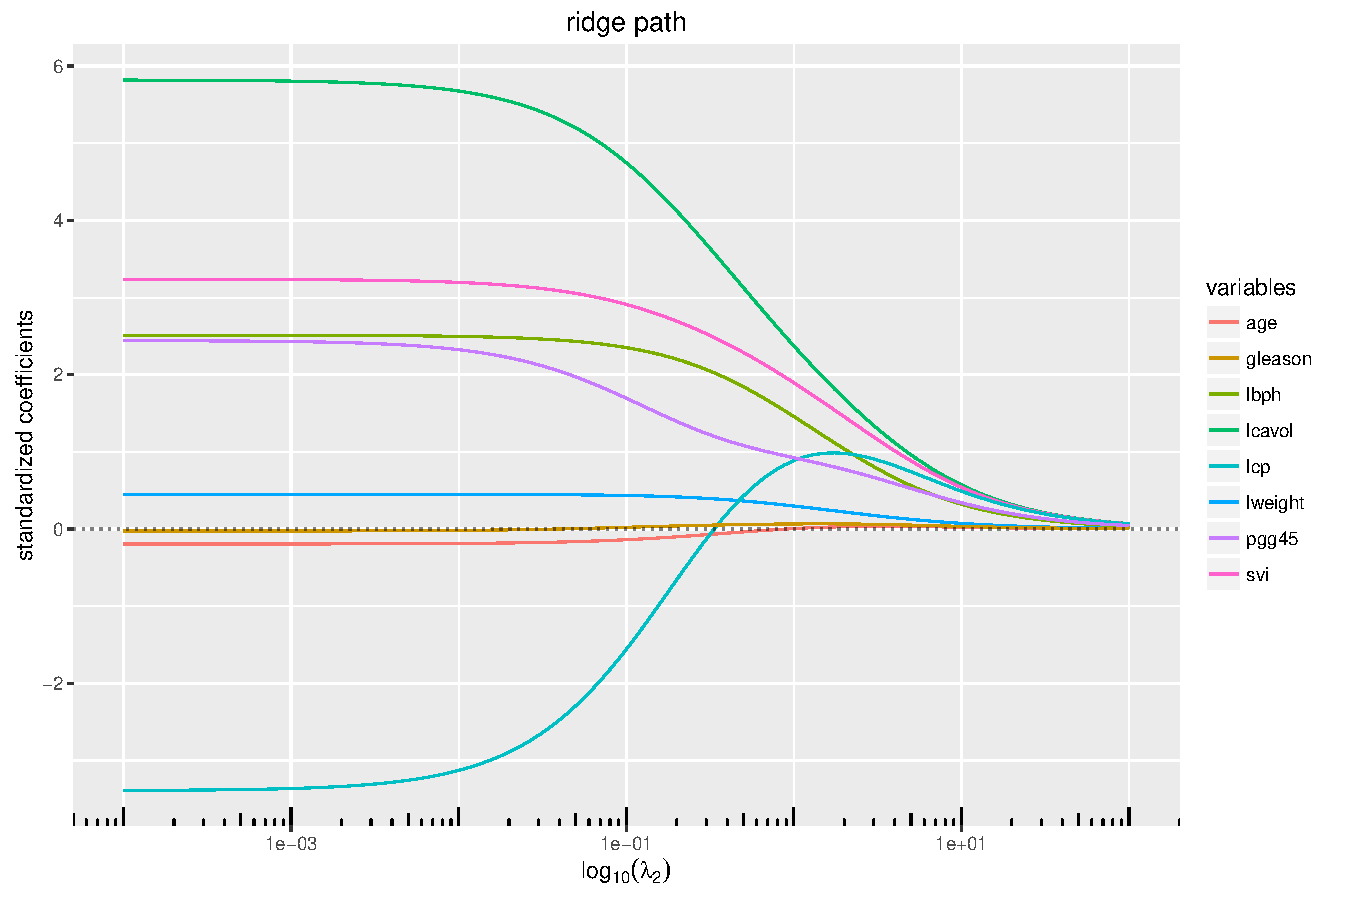
\includegraphics[width=\textwidth]{figures/toy_ridgeunnamed-chunk-50-2} 

\end{knitrout}
\end{frame}

\begin{frame}
  \frametitle{Ridge généralisée (I)}

  \begin{block}{Critère généralisé}
    \begin{align*}
      \hat{\bbeta}^{\text{ridge}} &  =   \argmin_{\bbeta\in\R^p}  \frac{1}{2}
      \|\mathbf{y} - \mathbf{X} \bbeta\|^2 + \lambda \bbeta^\intercal\bL\bbeta\\
      & = (\mathbf{X}^\intercal \mathbf{X} +
      \lambda \bL)^{-1} \mathbf{X}^\intercal \mathbf{y} = \mathbf{H}_{\lambda}^{\bL} \by.
    \end{align*}
    La matrice $\bL$ doit être semi-définie positive pour préserver la convexité.
  \end{block}

  \vfill

  \begin{block}{Résolution}<2>
    \begin{itemize}
      \item Considérons les données transformées $\bX \bC^{-1}$ où
    $\bC=\bL^{1/2}$  e.g.   par factorisation de Cholesky
    $\bC^T \bC = \bL$.
        \item Considérons la SVD  $\bU\bD\bV^T=\bX \bC^{-1}$ des données transformées
    \end{itemize}
    Alors
    \begin{equation*}
      \hatbbetaridge_{\bL}
      = \bC^{-1} \bV \left(\bD^2+\lambda\bI\right)^{-1}\bD \bU^T \by.
    \end{equation*}
  \end{block}

\end{frame}

\begin{frame}
  \frametitle{Ridge généralisée (II)}

  \begin{block}{Interpretation graphique}
    Soit $\mathcal{G} = (\mathcal{E}, \mathcal{V}, \mathcal{W})$ un graphe pondéré. Alors
    \begin{equation*}
      \sum_{\alert{(i,j)\in\mathcal{E}}} w_{ij}  (\beta_j-\beta_i)^2 =
    \bbeta^T \bL \bbeta,
    \end{equation*}
    où $\bL$ est la matrice \textit{Laplacienne} associé au graphe (semi-définie positive).
  \end{block}

  \vfill

  \begin{block}{Interpretation bayésienne}
    Supposons un prior Gaussien $\bbeta\sim\mathcal{N}(\mathbf{0},
    \tilde{\bX} = \bU\bD\bL^{-1})$, i.e.,
    \begin{equation*}
      \log\P(\bbeta|\bL) = \bbeta^T L \bbeta + cst.,
    \end{equation*}
    alors $\hatbbetaridge_{\bL}$ est la moyenne a posteriori (le mode).
  \end{block}

\end{frame}

\subsubsection{Choix du paramètre de régularisation}

\begin{frame}
   \frametitle{Les options classiques}

\begin{block}{En estimant l'erreur de prédiction}
On choisit le $\lambda$ minimisant l'erreur estimée
\begin{itemize}
\item par l'estimateur hold-out ou
\item par validation croisée.
\end{itemize}
\end {block}

\vfill

\begin{block}{Par critère pénalisé}
On choisit le $\lambda$ minimisant le critère de forme générale
\begin{equation*}
\mathrm{crit}(\lambda) = \mathrm{err}_\mathcal{D}(\lambda) + \mathrm{pen}(\mathrm{df}_\lambda)
\end{equation*}
$\rightsquigarrow$ Quel sens donner aux degrés de liberté pour la Ridge?
\end {block}

\end{frame}

\begin{frame}
 \frametitle{En estimant l'erreur de prédiction par validation croisée}
 \framesubtitle{Pour la régression: PRESS (\textit{predicted residual sum of squares})}

 \begin{block}{Principe}
   \vspace{-.25cm}
   \begin{enumerate}
   \item Partitionner les données en $K$ sous-ensembles,
   \item Utiliser successivement chaque sous-ensemble comme test,
   \item Calculer l'erreur de test pour les $K$ sous-ensembles,
   \item Moyenner les $K$ erreurs pour obtenir l'estimation finale.
   \end{enumerate}
 \end{block}

 \vspace{-.25cm}

 \begin{block}{Formalisme}<2>
   Soit  $\kappa  :   \{1,\dots,n\}  \rightarrow  \{1,\dots,K\}$  une
   fonction indicatrice de la partition de la $i$ème observation.  On
   note  $\hat{\bbeta}^{-k}$ les  paramètres estimés  sur les  données
   privées du $k$ième sous-ensemble. Alors
  \begin{equation*}
    \mathrm{CV}(\hat{\bbeta})     =    \frac{1}{n}\sum_{i=1}^n
    (y_i - x_i^T \hat{\bbeta}^{-\kappa(i)} )^2
  \end{equation*}
  donne  l'estimation  de  l'erreur   de  prédiction  par  validation
  croisée.
 \end{block}

\end{frame}

\begin{frame}
  \frametitle{Validation croisée: remarques et compléments}

  \begin{block}{Remarques}
    \begin{enumerate}
    \item Si $K=n$, LOOCV,
    \item Si $K=2$, estimation "hold-out",
    \item En grande dimension,  $K$ doit être choisi avec ``attention'',
    \item $CV(\lambda)$ calcule l'erreur de CV le long du chemin de régularisation.
    \end{enumerate}
  \end{block}

  \vfill
  
  \begin{proposition} Soit $\mathbf{H}$ une matrice de lissage (smoothing), i.e.,
    un opérateur linéaire fini tel que  $\hat{\by} = \mathbf{H} \by$. Alors l'erreur CV LOO vérifie
    \begin{equation*}
      \mathrm{CV}     =  \frac{1}{n}\sum_{i=1}^n
      (y_i - \hat{f}(x_i)^{-i})^2 = \frac{1}{n}\sum_{i=1}^n
      \left(\frac{y_i - \hat{f}(x_i)}{1-H_{ii}}\right)^2.
    \end{equation*}
  \end{proposition}

\end{frame}

\begin{frame}
  \frametitle{Degrés de liberté effectifs}

\begin{block}{Idées}
  \begin{itemize}
  \item Les degrés de liberté décrivent le  niveau de complexité d'un modèle .
  \item Pour l'OLS, $\mathrm{df} = p$ (plus 1 pour la constante).
  \end{itemize}
\end{block}

  \vfill

  \begin{definitionf} Considérons une prédiction 
    $\hat{\mathbf{y}}$ ajustée depuis une observation $\mathbf{y}$. Les degrés de liberté généralisés de la prédiction sont définis par 
    \begin{equation*}
      \mathrm{df}(\hat{\mathbf{y}})    =    \frac{1}{\sigma^2}
      \sum_{i=1}^n \mathrm{cov}(\hat{y}_i,y_i).
    \end{equation*}
    $\rightsquigarrow$ Plus l'ajustement est proche des données, plus le modèle est complexe, plus grande est la covariance.
  \end{definitionf}

\end{frame}

\begin{frame}
  \frametitle{Degrés de liberté effectifs: cas de la Ridge}

  \begin{proposition} Considérons une méthode linéaire qui s'écrive:
    \begin{equation*}
      \hat{\mathbf{y}} = \mathbf{H} \mathbf{y}.
    \end{equation*}
    Les degrés de liberté effectifs du     modèle      $\hat{\mathbf{y}}$ vérifient
    \begin{equation*}
      \mathrm{df}(\hat{\mathbf{y}}) = \mathrm{Tr}(\mathbf{H}).
    \end{equation*}
  \end{proposition}

  \vfill

  \begin{block}{Ridge}
    Pour la régression Ridge, $\mathrm{df}$ est une fonction décroissant de 
    $\lambda$ qui tend vers 0 (ou 1 en considérant la constante):
    \begin{equation*}
      \mathrm{df}(\hat{\mathbf{y}}_\lambda) =\sum_{i=1}^p \frac{d_i^2}{d_i^2+\lambda},
    \end{equation*}
  \end{block}


\end{frame}


\begin{frame}[containsverbatim]
  \frametitle{Cancer de la prostate}
  \framesubtitle{Calcul de l' AIC/BIC en estimant $\sigma$}

\begin{knitrout}\scriptsize
\definecolor{shadecolor}{rgb}{0.969, 0.969, 0.969}\color{fgcolor}\begin{kframe}
\begin{alltt}
\hlstd{crit} \hlkwb{<-} \hlkwd{criteria}\hlstd{(ridge.path,} \hlkwc{plot}\hlstd{=}\hlnum{FALSE}\hlstd{)}
\hlkwd{print}\hlstd{(}\hlkwd{head}\hlstd{(crit}\hlopt{$}\hlstd{criterion),} \hlkwc{digits}\hlstd{=}\hlnum{3}\hlstd{)}
\end{alltt}
\begin{verbatim}
##    AIC  BIC     GCV df   lambda fraction
## 1 3.77 3.78 0.00575  9 0.000100        1
## 2 3.77 3.78 0.00575  9 0.000115        1
## 3 3.77 3.78 0.00575  9 0.000132        1
## 4 3.77 3.78 0.00575  9 0.000152        1
## 5 3.77 3.78 0.00575  9 0.000175        1
## 6 3.77 3.78 0.00575  9 0.000201        1
\end{verbatim}
\begin{alltt}
\hlkwd{print}\hlstd{(}\hlkwd{head}\hlstd{(crit}\hlopt{$}\hlstd{beta.min))}
\end{alltt}
\begin{verbatim}
## 6 x 2 Matrix of class "dgeMatrix"
##                AIC        BIC
## lcavol   0.8635928  0.8635928
## lweight  0.4152738  0.4152738
## age     -0.1520864 -0.1520864
## lbph     0.2911599  0.2911599
## svi      0.4092488  0.4092488
## lcp     -0.2047139 -0.2047139
\end{verbatim}
\end{kframe}
\end{knitrout}
\end{frame}


\begin{frame}[containsverbatim]
  \frametitle{Cancer de la prostate}
  \framesubtitle{Calcul de l' AIC/BIC en estimant $\sigma$ (plot)}

\begin{knitrout}\scriptsize
\definecolor{shadecolor}{rgb}{0.969, 0.969, 0.969}\color{fgcolor}
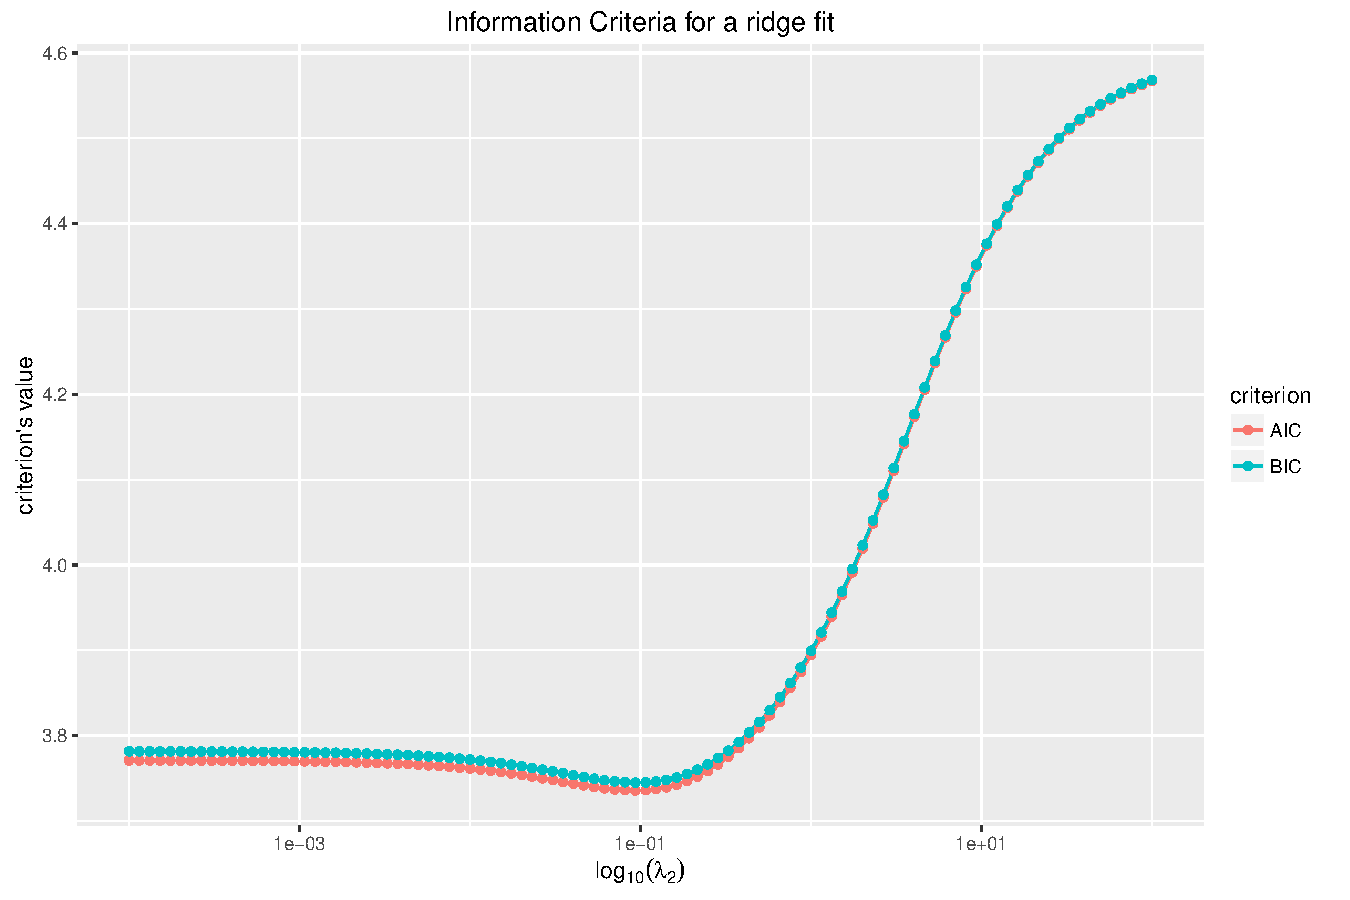
\includegraphics[width=\textwidth]{figures/toy_ridgeunnamed-chunk-52-1} 

\end{knitrout}
\end{frame}

\begin{frame}[containsverbatim]
  \frametitle{Cancer de la prostate}
  \framesubtitle{Calcul de l' AIC/BIC en estimant $\sigma$ (plot 2)}

\begin{knitrout}\scriptsize
\definecolor{shadecolor}{rgb}{0.969, 0.969, 0.969}\color{fgcolor}
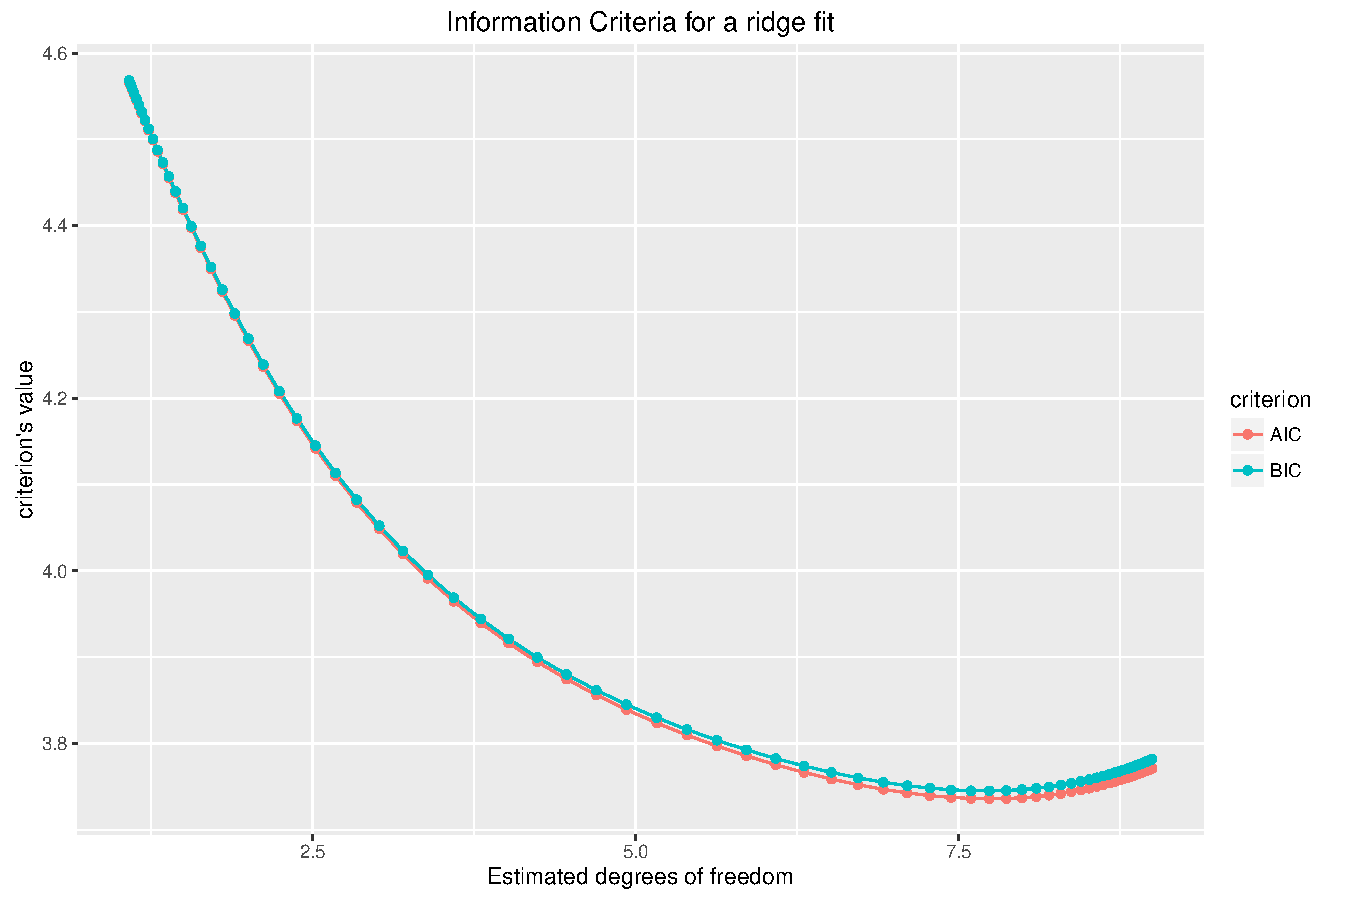
\includegraphics[width=\textwidth]{figures/toy_ridgeunnamed-chunk-53-1} 

\end{knitrout}
\end{frame}

\begin{frame}[containsverbatim]
  \frametitle{Validation croisée}

  La validation croisée se parallèlise facilement et ne prend que peu de temps sur un petit jeu de données

\begin{knitrout}\scriptsize
\definecolor{shadecolor}{rgb}{0.969, 0.969, 0.969}\color{fgcolor}\begin{kframe}
\begin{alltt}
\hlkwd{system.time}\hlstd{(loo} \hlkwb{<-} \hlstd{quadrupen}\hlopt{::}\hlkwd{crossval}\hlstd{(x.train,y.train,}\hlstr{"ridge"}\hlstd{,}\hlkwc{K}\hlstd{=n,}\hlkwc{normalize}\hlstd{=}\hlnum{FALSE}\hlstd{))}
\end{alltt}
\begin{verbatim}
## 
## CROSS-VALIDATION FOR  ridge  REGULARIZER 
## 
## 67-fold CV on the lambda2 grid.
##    user  system elapsed 
##   0.708   0.256   0.330
\end{verbatim}
\end{kframe}
\end{knitrout}

\begin{knitrout}\scriptsize
\definecolor{shadecolor}{rgb}{0.969, 0.969, 0.969}\color{fgcolor}\begin{kframe}
\begin{alltt}
\hlkwd{system.time}\hlstd{(CV10} \hlkwb{<-} \hlstd{quadrupen}\hlopt{::}\hlkwd{crossval}\hlstd{(x.train,y.train,}\hlstr{"ridge"}\hlstd{,}\hlkwc{K}\hlstd{=}\hlnum{10}\hlstd{,}\hlkwc{normalize}\hlstd{=}\hlnum{FALSE}\hlstd{))}
\end{alltt}
\begin{verbatim}
## 
## CROSS-VALIDATION FOR  ridge  REGULARIZER 
## 
## 10-fold CV on the lambda2 grid.
##    user  system elapsed 
##   0.472   0.636   0.260
\end{verbatim}
\end{kframe}
\end{knitrout}

\end{frame}

\begin{frame}[containsverbatim]
  \frametitle{Validation croisée ("leave one out")}
\begin{knitrout}\scriptsize
\definecolor{shadecolor}{rgb}{0.969, 0.969, 0.969}\color{fgcolor}
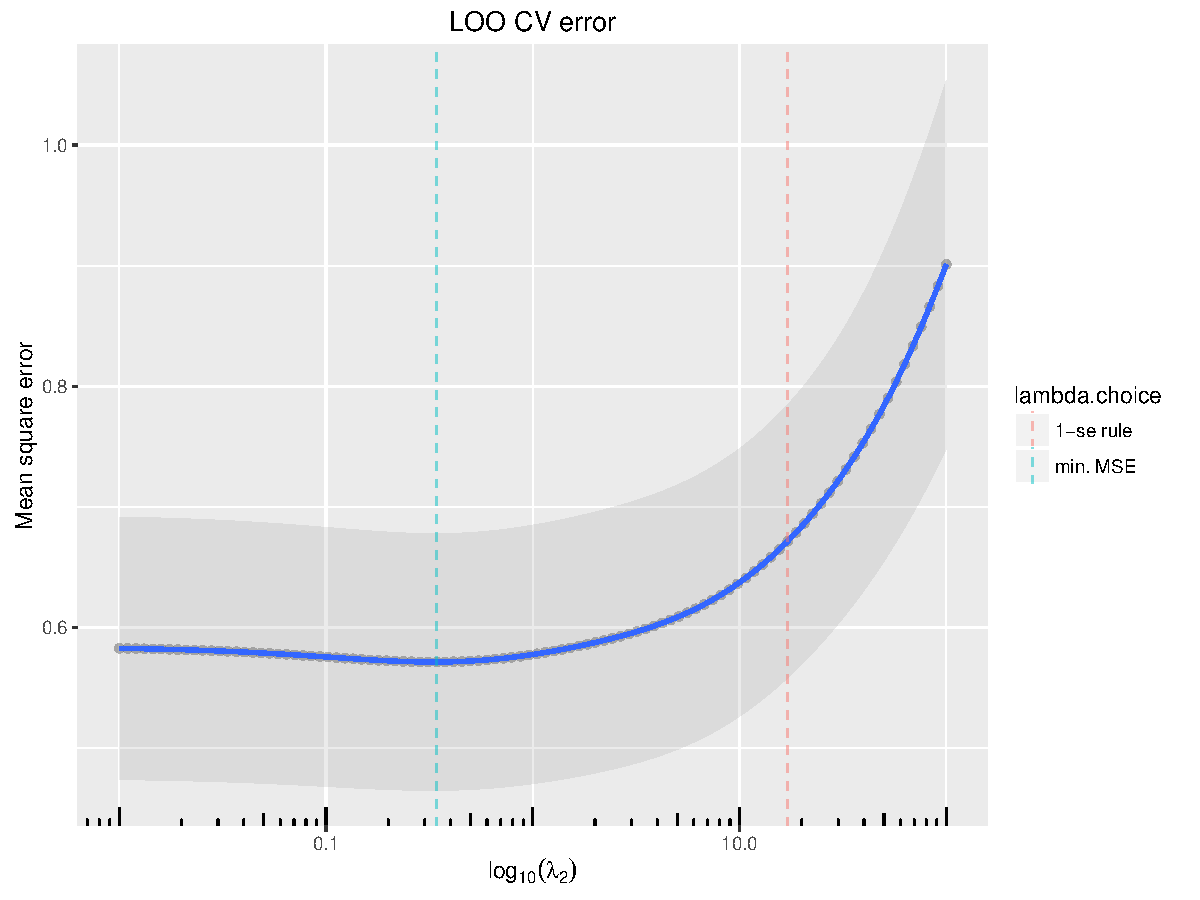
\includegraphics[width=\textwidth]{figures/toy_ridgeunnamed-chunk-56-1} 

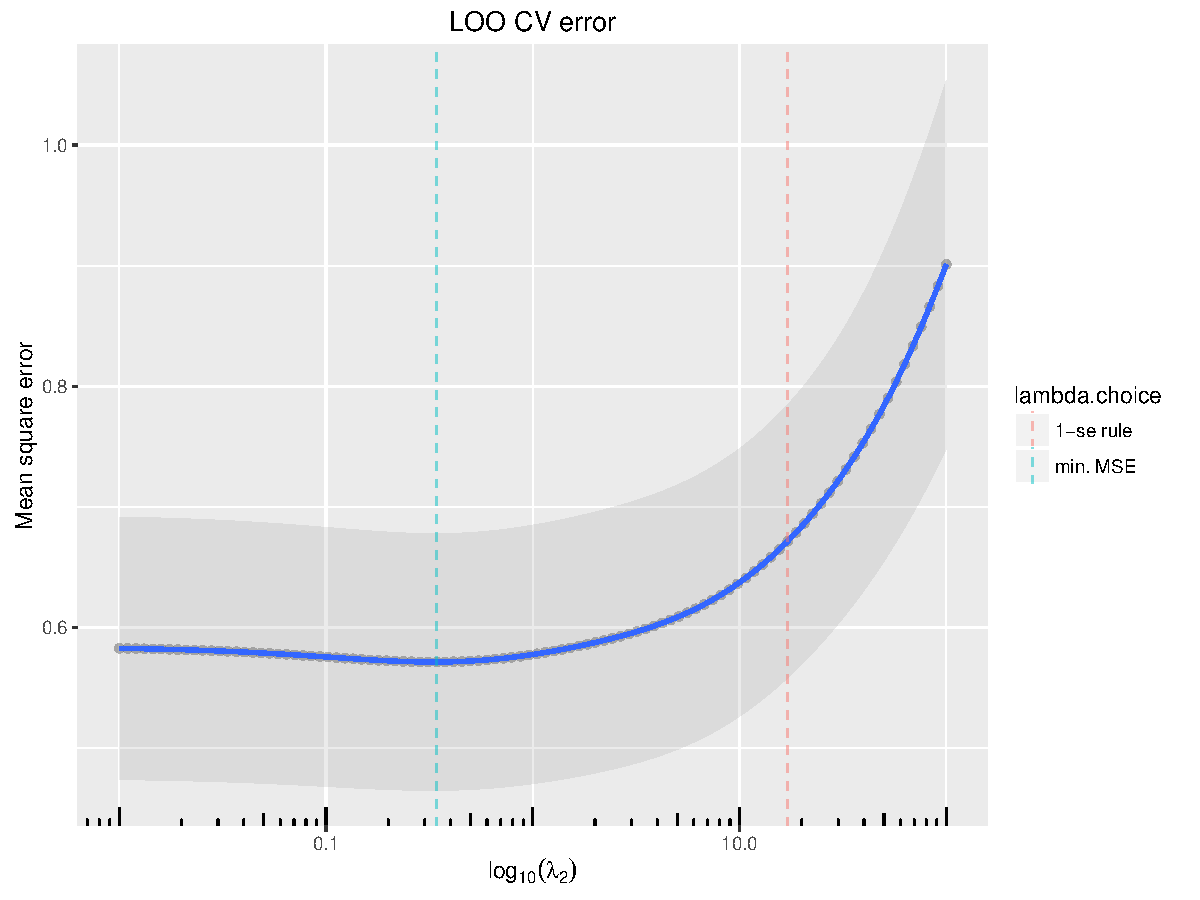
\includegraphics[width=\textwidth]{figures/toy_ridgeunnamed-chunk-56-2} 

\end{knitrout}
\end{frame}



\begin{frame}[containsverbatim]
  \frametitle{Validation croisée ("ten fold")}
\begin{knitrout}\scriptsize
\definecolor{shadecolor}{rgb}{0.969, 0.969, 0.969}\color{fgcolor}
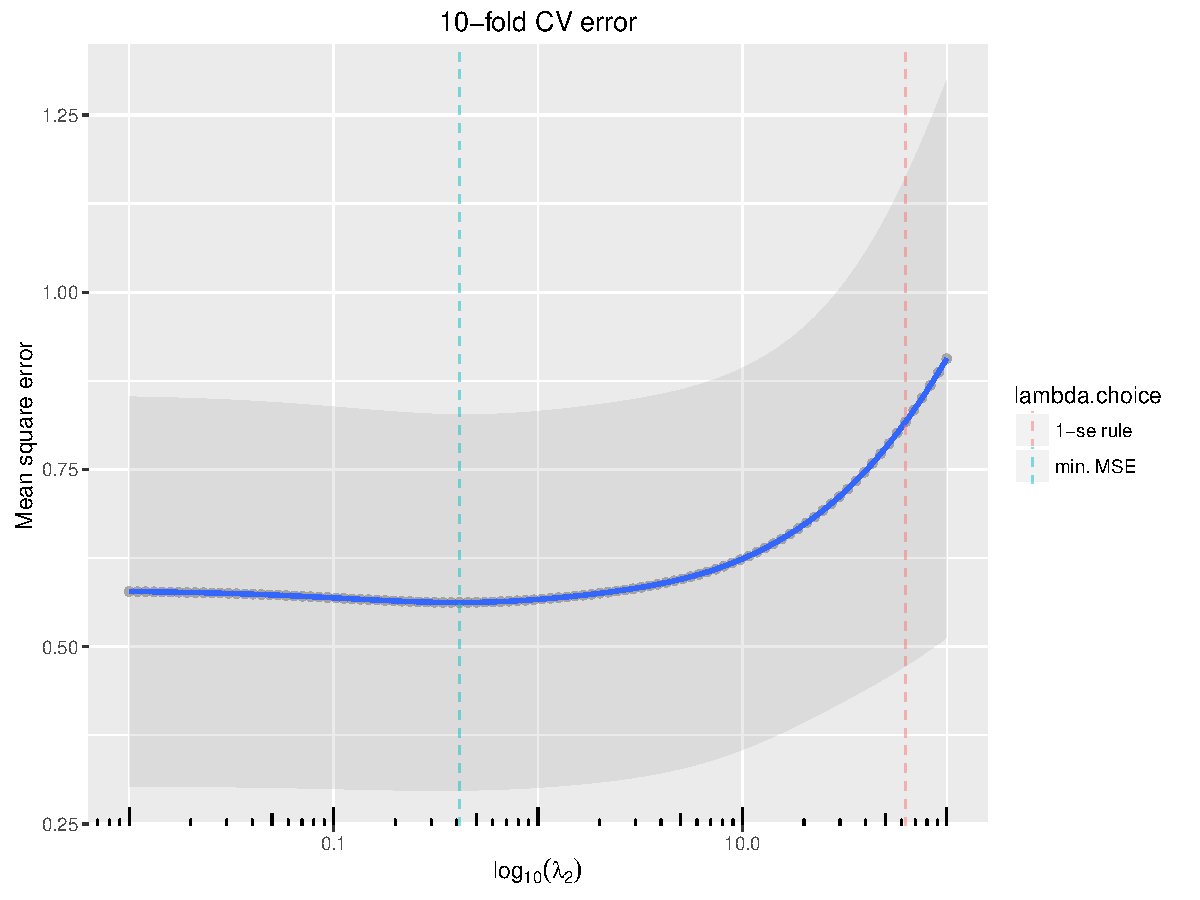
\includegraphics[width=\textwidth]{figures/toy_ridgeunnamed-chunk-57-1} 

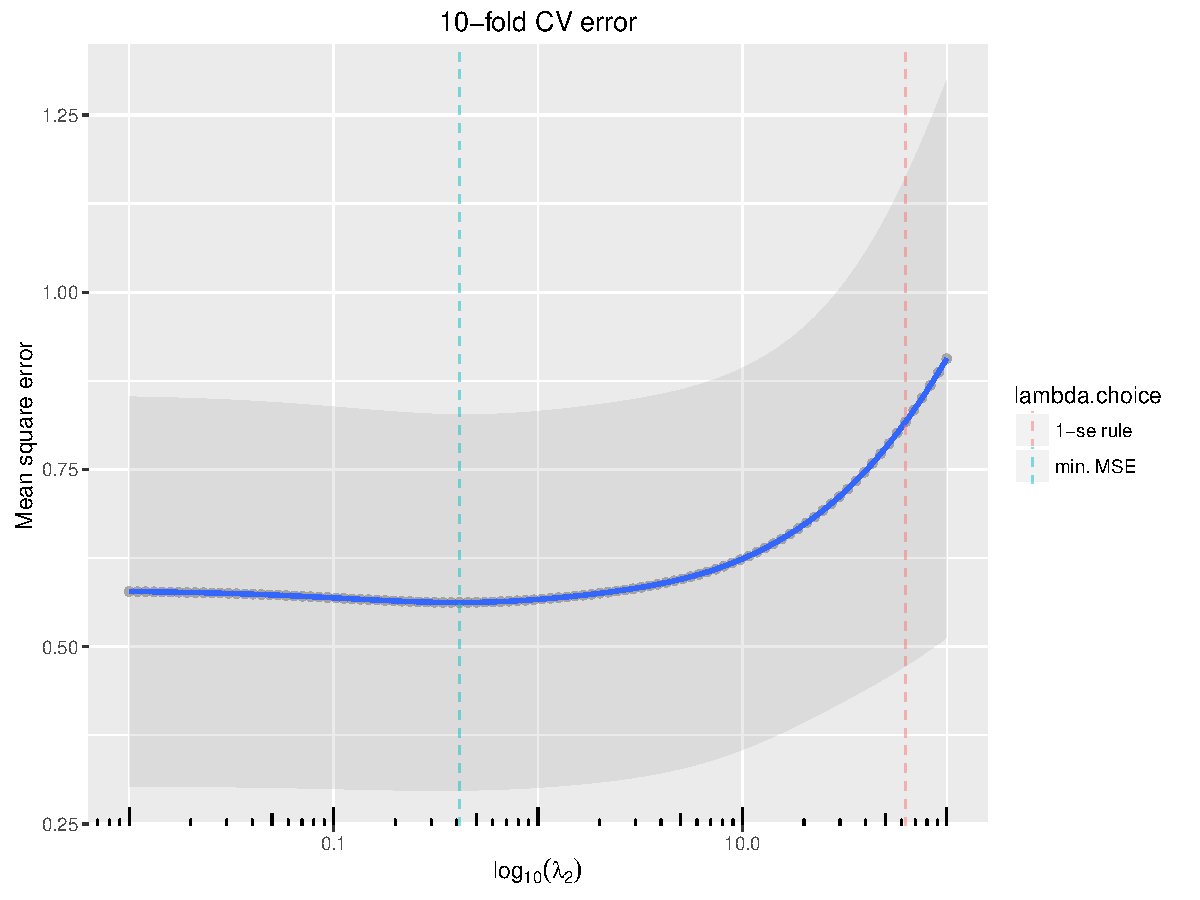
\includegraphics[width=\textwidth]{figures/toy_ridgeunnamed-chunk-57-2} 

\end{knitrout}
\end{frame}






\subsection{Régression Lasso}

\subsubsection{Définition de l'estimateur}

\begin{frame}
  \frametitle{Le Lasso}
  \framesubtitle{Least Absolute Shrinkage and Selection Operator}

  \begin{block}{Limite de la ridge}
    La Ridge  régularise\dots mais on aimerait également sélectionner les prédicteurs significatifs.
  \end{block}

  \vfill

  \begin{block}{Idée}
    Proposer  une  contrainte  qui  force  la  \alert{parcimonie}  (en
    forçant des entrées de $\hatbbeta$ à zéro).
  \end{block}

  \vfill

  \onslide<2>{
  \begin{overlayarea}{\textwidth}{.4\textheight}
    \begin{columns}
      \begin{column}[c]{.6\textwidth}
        \begin{block}{Le Lasso comme problème d'optimisation}
          Le Lasso estime $\hat{\bbeta}^{\text{lasso}}$ via
          \begin{equation*}
            \minimize_{\bbeta\in\R^{p+1}} \mathrm{RSS}(\bbeta), \quad \text{s.t.  }  \sum_{j=1}^p
            \left|\beta_j\right|  \leq s,
          \end{equation*}
          où $s$ est un niveau de régularisation.
        \end{block}
      \end{column}
      \begin{column}{.4\textwidth}
        \includegraphics<2>{figures/lasso_set}
      \end{column}
    \end{columns}
  \end{overlayarea}
  }
\end{frame}

\pgfdeclareimage[height=0.8\textheight]{sparsity_loss}{figures/sparsity_loss}
\pgfdeclareimage[height=0.5\textheight]{sparsity_proj}{figures/sparsity_proj}
\pgfdeclareimage[height=0.375\textheight]{sparsity6}{figures/sparsity_6}
\pgfdeclareimage[height=0.375\textheight]{sparsity8bis}{figures/sparsity_8bis}
\pgfdeclareimage[height=0.375\textheight]{sparsity9}{figures/sparsity_9}
\pgfdeclareimage[height=0.375\textheight]{sparsity10}{figures/sparsity_10}
\pgfdeclareimage[height=0.375\textheight]{sparsity11}{figures/sparsity_11}
\pgfdeclareimage[height=0.375\textheight]{sparsity12}{figures/sparsity_12}

\begin{frame}
  \frametitle{Interprétation géométrique de la parcimonie}

  \begin{columns}
    \begin{column}{0.425\textwidth}
      \begin{tikzpicture}
        \only<1>{%
          \node (Surf2) at (0,0) {\pgfuseimage{sparsity_loss}}
          node    at    (Surf2.west)    [rotate=90,yshift=5mm]
          {$\ell(\beta_1,\beta_2)$}
          node at (Surf2.south west) [xshift=5mm,yshift=5mm]{$\beta_2$}
          node at (Surf2.south east) [xshift=-7.5mm,yshift=2.5mm]{$\beta_1$};
        }
        \only<2>{%
          \node (titi) at (0,0) {\phantom{titi}};
          \node (Surf3) at (0,-4.5) {\pgfuseimage{sparsity_proj}}
          node at (Surf3.west) [rotate=90,yshift=2.5mm] {$\beta_2$}
          node at (Surf3.south) [yshift=-2.5mm] {$\beta_1$};
        }
      \end{tikzpicture}
    \end{column}
    \begin{column}{.6\textwidth}
      
      \begin{equation*}
        \begin{gathered}
          \begin{array}{rl} 
            \displaystyle \maximize_{\beta_1,\beta_2} & \ell(\beta_1,\beta_2) \\
            \mathrm{s.c.} & \Omega(\beta_1,\beta_2) \leq c 
          \end{array}
          \\
          \Updownarrow
          \\
          \begin{array}{rl} 
            \displaystyle \minimize_{\beta_1,\beta_2} & -\ell(\beta_1,\beta_2) \\
            \mathrm{s.c.} & \Omega(\beta_1,\beta_2) \leq c 
          \end{array}
          \\
          \Updownarrow
          \\
          \minimize_{\beta_1,\beta_2} -\ell(\beta_1,\beta_2) + \lambda
          \Omega(\beta_1,\beta_2)\\
        \end{gathered}
      \end{equation*}
    \end{column}
  \end{columns}
\end{frame}


\pgfdeclareimage[height=0.375\textheight]{sparsity6}{figures/sparsity_6}
\pgfdeclareimage[height=0.375\textheight]{sparsity8bis}{figures/sparsity_8bis}
\pgfdeclareimage[height=0.375\textheight]{sparsity9}{figures/sparsity_9}
\pgfdeclareimage[height=0.375\textheight]{sparsity10}{figures/sparsity_10}
\pgfdeclareimage[height=0.375\textheight]{sparsity11}{figures/sparsity_11}
\pgfdeclareimage[height=0.375\textheight]{sparsity12}{figures/sparsity_12}


\begin{frame}
  \frametitle{Interprétation géométrique de la parcimonie}
  \framesubtitle{Cône de dualité}

  {\centerline{généralise la notion de de vecteur normal}}

  \bigskip

  \begin{overlayarea}{\textwidth}{\textheight}


    \begin{tikzpicture}
      \only<1>{%
      \node (Surf2) at (0,0) {\pgfuseimage{sparsity6}}
              node at (Surf2.west) [rotate=90,yshift=2.5mm] {$\beta_2$}
              node at (Surf2.south) [yshift=-1mm] {$\beta_1$};
      }
      \only<1-2>{%
      \node (Surf3) at (4,0) {\pgfuseimage{sparsity8bis}}
              node at (Surf3.west) [rotate=90,yshift=2.5mm] {$\beta_2$}
              node at (Surf3.south) [yshift=-1mm] {$\beta_1$};
      }
      \only<1-3>{%
        \node (Surf4) at (8,0) {\pgfuseimage{sparsity9}}
                node at (Surf4.west) [rotate=90,yshift=2.5mm] {$\beta_2$}
                node at (Surf4.south) [yshift=-1mm] {$\beta_1$};
      }
      \only<4>{%
        \node (Surf5) at (8,0) {\pgfuseimage{sparsity10}}
                node at (Surf5.west) [rotate=90,yshift=2.5mm] {$\beta_2$}
                node at (Surf5.south) [yshift=-1mm] {$\beta_1$};
      }
      \only<3->{%
        \node (Surf6) at (4,0) {\pgfuseimage{sparsity11}}
                node at (Surf6.west) [rotate=90,yshift=2.5mm] {$\beta_2$}
                node at (Surf6.south) [yshift=-1mm] {$\beta_1$};
      }
      \only<2->{%
        \node (Surf7) at (0,0) {\pgfuseimage{sparsity12}}
                node at (Surf7.west) [rotate=90,yshift=2.5mm] {$\beta_2$}
                node at (Surf7.south) [yshift=-1mm] {$\beta_1$};
      }
    \end{tikzpicture}

    \medskip

    Soit $C$ un ensemble convexe,
    \begin{itemize}
    \item  $C^\star(x_0) =  \set{y|y^T(x-x_0) \geq  0,x\in C}$  est le
      cône dual en $x_0$,
    \item $N_C(x_0) = \set{y|y^T(x-x_0) \leq 0,x\in C}$ est le cône normal, 
    \end{itemize}

    \medskip

    \only<4>{%
      {\centerline{Forme des cônes $\Rightarrow$ pattern de parcimonie}}
    }

  \end{overlayarea}
\end{frame}




\begin{frame}
  \frametitle{Les singularités induisent de la "sparsité"}
  \framesubtitle{Figures de Sylvie Huet}

  \begin{overlayarea}{\textwidth}{\textheight}

    \begin{equation*}
      \sum_{i=1}^n (y_i-x_i^1\beta_1 - x_i^2\beta_2)^2, \qquad
      \only<1>{\text{pas de constrainte}}
      \only<2>{\text{s.c. } |\beta_1| + |\beta_2| < 0.75}
      \only<3>{\text{s.c. } |\beta_1| + |\beta_2| < 0.66}
      \only<4>{\text{s.c. } |\beta_1| + |\beta_2| < 0.4}
      \only<5>{\text{s.c. } |\beta_1| + |\beta_2| < 0.2}
      \only<6>{\text{s.c. } |\beta_1| + |\beta_2| < 0.0743}
    \end{equation*}

    \includegraphics<1>{figures/dess11}
    \includegraphics<2>{figures/dess12}
    \includegraphics<3>{figures/dess13}
    \includegraphics<4>{figures/dess14}
    \includegraphics<5>{figures/dess15}
    \includegraphics<6>{figures/dess16}

  \end{overlayarea}

\end{frame}

\begin{frame}
  \frametitle{Le Lasso comme méthode de régression pénalisée}

  \begin{block}{}
    On ne pénalise pas la constante, donc
    \begin{itemize}
    \item $\hat{\beta}_0 = \bar{\mathbf{y}}$,
    \item on centre $\mathbf{y}$ et $\mathbf{x}_j$, $j=1,\dots,p$,
    \item on normalise les prédicteurs avant d'ajuster,
    \item on renvoie  $\hatbbeta$ dans l'échelle d'origine.
    \end{itemize}
  \end{block}

  \vfill

 Résolution d'un problème d'optimisaiton convexe
  \begin{equation*}
      \hat{\bbeta}^{\text{lasso}}   =   \argmin_{\bbeta\in\R^p}  \frac{1}{2}
      \|\mathbf{y} - \mathbf{X} \bbeta\|^2 + \lambda \|\bbeta\|_1,
  \end{equation*}
  Pas de forme close, mais existe toujours et est unique lorsque $\mathbf{X}^\intercal \mathbf{X}$ est de plein rang.

  \vfill

  $\rightsquigarrow$  Le Lasso régularise et sélectionne les prédicteurs, mais n'a pas de solution explicite.

\end{frame}



\subsubsection{Propriétés et résolution pratique}

\begin{frame}
  \frametitle{Cas orthogonal et connexion avec l'OLS}
  
  À supposer que $\mathbf{X}^\intercal \mathbf{X} = \mathbf{I}$, alors
    \begin{columns}
      \begin{column}{.4\textwidth}
        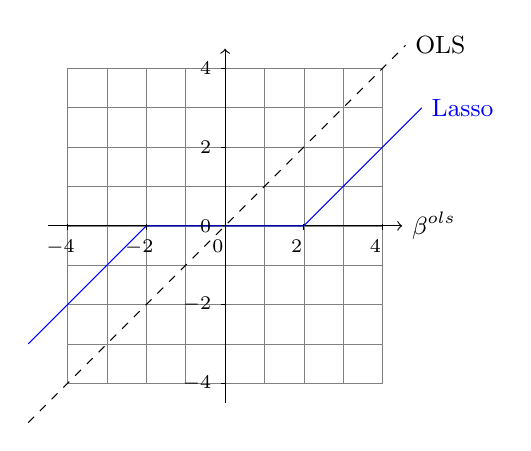
\begin{tikzpicture}[scale=.5,font=\small]
          \draw[very thin,color=gray] (-4,-4) grid [xstep=1,ystep=1] (4,4);
          \draw[->] (-4.5,0) -- (4.5,0) node[right] {$\beta^{\text{ols}}$};
          \draw[->] (0,-4.5) -- (0,4.5) ;
          \draw[color=blue] plot[samples=200] (\x,{max(0,1-2/abs(\x))*\x})
          node[right] {Lasso};
          \draw[dashed,color=black] plot (\x,{\x}) node[right] {OLS};

          % units for cartesian reference frame
          \foreach \x in {-4,-2,0,2,4}{
            \draw (\x cm,1pt)  -- (\x cm,-3pt)
            node[anchor=north,xshift=-0.09cm] {\scriptsize$\x$};
            \draw (1pt,\x cm) -- (-3pt,\x cm)
            node[anchor=east] {\scriptsize$\x$};
          }
        \end{tikzpicture}
      \end{column}

      \begin{column}{.55\textwidth}
          \begin{small}
            \begin{align*}
              \hatbeta_j^{\text{lasso}} & = \left( 1-\frac{\lambda}{\left|
                    \hatbeta_j^{\text{ols}}  \right|}  \right)^{\!\!+}
              \\
              & = S_{\text{thres}}(\hatbeta_j^{\text{ols}}, \lambda),
              \hatbeta_j^{\text{ols}} \enspace,
            \end{align*}
            \begin{equation*}
              \left| \hatbeta_j^{\text{lasso}} \right| = \left(
                \left| \hatbeta_j^{\text{ols}} \right| - \lambda
              \right)^{\!\!+}
              \enspace.
            \end{equation*}
          \end{small}
        \end{column}
    \end{columns}

$\rightsquigarrow$  correspond au  \alert{``seuillage-doux''}
    $S_{\text{thres}}$ de  Donoho et al.

\end{frame}

\begin{frame}
  \frametitle{Notion de sous-gradient et résolution}
  
  Un vecteur $\bbeta$ est solution du Lasso si et seulement si
  \begin{equation*}
    -\mathbf{X}^\intercal  (\mathbf{X}\bbeta  -  \mathbf{y}) +  \lambda
    {\boldsymbol\theta} = \mathbf{0}, \quad \text{with } 
     \left\{\begin{array}{ll}
         \theta_j = \mathrm{sign}(\beta_j) & \text{ if } \beta_j \neq 0, \\
        \theta_j \in [-1,1] & \text{ if } \beta_j = 0. \\
      \end{array}\right.
  \end{equation*}
  
  \vfill
  
  \begin{columns}[c]
    
    \begin{column}{.5\textwidth}
      \begin{tikzpicture}[scale=.5,font=\small]
        \node at (0,0) [circle,fill=black] {};
        \draw[<->] (-4.5,0) -- (4.5,0) node[right] {$\beta$}; 
        \draw[->] (0,0) -- (0,5.5)  node[left] {$|\beta|$}; 
        \draw[color=blue] plot[samples=200] (\x,{abs(\x)}) node[right] {};
      \end{tikzpicture}  
    \end{column}  
    
    \begin{column}{.5\textwidth}
      \begin{tikzpicture}[scale=.25,xscale=2,font=\small]
        \draw[<->] (-4.5,0) -- (4.5,0) node[right] {$\beta$}; 
        \draw[<->] (0,-5.5) -- (0,5.5) node[left] {$\mathrm{sign}(\beta)$}; 
        \draw[color=blue] (-4.5,-5.5) -- (0,-5.5) ;
        \draw[color=blue] (0,5.5) -- (4.5,5.5) ;
      \end{tikzpicture}  
    \end{column}

  \end{columns}

  \vfill

  \begin{thebibliography}{99}
    \setbeamertemplate{bibliography item}[book]    
  \bibitem[boyd]{boyd} Boyd, S. and Vandenberghe, L. 2006. Convex optimization.
  \end{thebibliography}
\end{frame}

\begin{frame}
  \frametitle{L'algorithme de shooting}

  \begin{thebibliography}{99}
  \bibitem[fu]{fu} Fu, W., 1998.
    \newblock Penalized regressions: the bridge vs. the lasso.
  \end{thebibliography}

  \vfill

  Soit
  \begin{equation*}
    S(x,\lambda) = \mathrm{sign}(x) \max(0, |x|-\lambda ).
  \end{equation*}
  l'opérateur de seuillage doux.
 
  \begin{enumerate}
  \item Start with $\hat{\bbeta} = \bbeta^{\text{ols}}$
  \item For each $j=1,\dots,p$, set
    \begin{equation*}
      \hat{\beta}_j     =     S\left(\sum_{i=1}^n    x_{ij}(y_i     -
        \tilde{y}_i^{(j)}) ,\lambda \right) / 
      \mathbf{x}_j^\intercal \mathbf{x}_j,
    \end{equation*}
    with $\tilde{y}_i^{(j)} = \sum_{k\neq j} x_{ik} \hat{\beta}_k$.
  \item Repeat 2 until convergence
  \end{enumerate}
\end{frame}

\begin{frame}
  \frametitle{LARs: Least angle regression}
\framesubtitle{Une méthode populaire pour ajuster le Lasso}
  \begin{thebibliography}{99}
  \bibitem[lars]{lars}   B.   Efron,    T.   Hastie,   I.   Johnstone,
    R. Tibshirani, 2004. \newblock Least Angle Regression.
  \end{thebibliography}

  \vfill
  
  \begin{block}{Algorithme efficace de calcuyl du chemin de solution}
    La solution du  LARS  consiste en une fonction  décrivant
    $\hatbbeta$ pour chaque valeur de  $\lambda$.
    
    \begin{itemize}
    \item  construit un chemin   \textit{linéaire par morceau}  de la solution en aprtant du vecteur nul,
    \item Coût proche de celui de l'OLS, 
    \item bien adapté à la validation croisée.
    \end{itemize}
  \end{block}
    
\end{frame}




\begin{frame}[containsverbatim,allowframebreaks]
  \frametitle{Lasso sur données  cancer de la prostate}

  \vfill
Calcul du chemin de solution du Lasso

\begin{knitrout}\scriptsize
\definecolor{shadecolor}{rgb}{0.969, 0.969, 0.969}\color{fgcolor}\begin{kframe}
\begin{alltt}
\hlkwd{library}\hlstd{(quadrupen)}
\hlstd{lasso.path} \hlkwb{<-} \hlstd{quadrupen}\hlopt{::}\hlkwd{lasso}\hlstd{(x.train,y.train)}
\end{alltt}
\end{kframe}
\end{knitrout}

\vfill

Calcul de l'erreur de prédiction sur l'ensemble test
\begin{knitrout}\scriptsize
\definecolor{shadecolor}{rgb}{0.969, 0.969, 0.969}\color{fgcolor}\begin{kframe}
\begin{alltt}
\hlstd{err} \hlkwb{<-} \hlkwd{colMeans}\hlstd{((y.test}\hlopt{-}\hlkwd{predict}\hlstd{(lasso.path,x.test))}\hlopt{^}\hlnum{2}\hlstd{)}
\end{alltt}
\end{kframe}
\end{knitrout}

\vfill

On choisit $\lambda^\star$ minimisant cette erreur
\begin{knitrout}\scriptsize
\definecolor{shadecolor}{rgb}{0.969, 0.969, 0.969}\color{fgcolor}\begin{kframe}
\begin{alltt}
\hlstd{lasso.path}\hlopt{@}\hlkwc{lambda1}\hlstd{[}\hlkwd{which.min}\hlstd{(err)]}
\end{alltt}
\begin{verbatim}
## [1] 0.9291339
\end{verbatim}
\end{kframe}
\end{knitrout}

\framebreak

L'erreur de prédiction est significativement plus petite que pour l'OLS et la ridge, avec seulement 5 coefficients + la constante
\begin{knitrout}\scriptsize
\definecolor{shadecolor}{rgb}{0.969, 0.969, 0.969}\color{fgcolor}\begin{kframe}
\begin{alltt}
\hlstd{err[}\hlkwd{which.min}\hlstd{(err)]}
\end{alltt}
\begin{verbatim}
##     0.929 
## 0.4447334
\end{verbatim}
\begin{alltt}
\hlstd{lasso.path}\hlopt{@}\hlkwc{coefficients}\hlstd{[}\hlkwd{which.min}\hlstd{(err), ]}
\end{alltt}
\begin{verbatim}
##     lcavol    lweight        age       lbph        svi        lcp 
## 0.83764934 1.74070516 0.00000000 0.09308986 0.18471854 0.00000000 
##    gleason      pgg45 
## 0.00000000 0.07755607
\end{verbatim}
\end{kframe}
\end{knitrout}

\end{frame}

\begin{frame}[containsverbatim]
  \frametitle{Erreur de prédiction sur les données test}

\begin{knitrout}\scriptsize
\definecolor{shadecolor}{rgb}{0.969, 0.969, 0.969}\color{fgcolor}\begin{kframe}
\begin{alltt}
\hlkwd{qplot}\hlstd{(}\hlkwd{log10}\hlstd{(lasso.path}\hlopt{@}\hlkwc{lambda1}\hlstd{), err)} \hlopt{+} \hlkwd{geom_line}\hlstd{()} \hlopt{+}
\hlkwd{geom_vline}\hlstd{(}\hlkwc{xintercept}\hlstd{=}\hlkwd{log10}\hlstd{(lasso.path}\hlopt{@}\hlkwc{lambda1}\hlstd{[}\hlkwd{which.min}\hlstd{(err)]),} \hlkwc{lty}\hlstd{=}\hlnum{3}\hlstd{)}
\end{alltt}
\end{kframe}
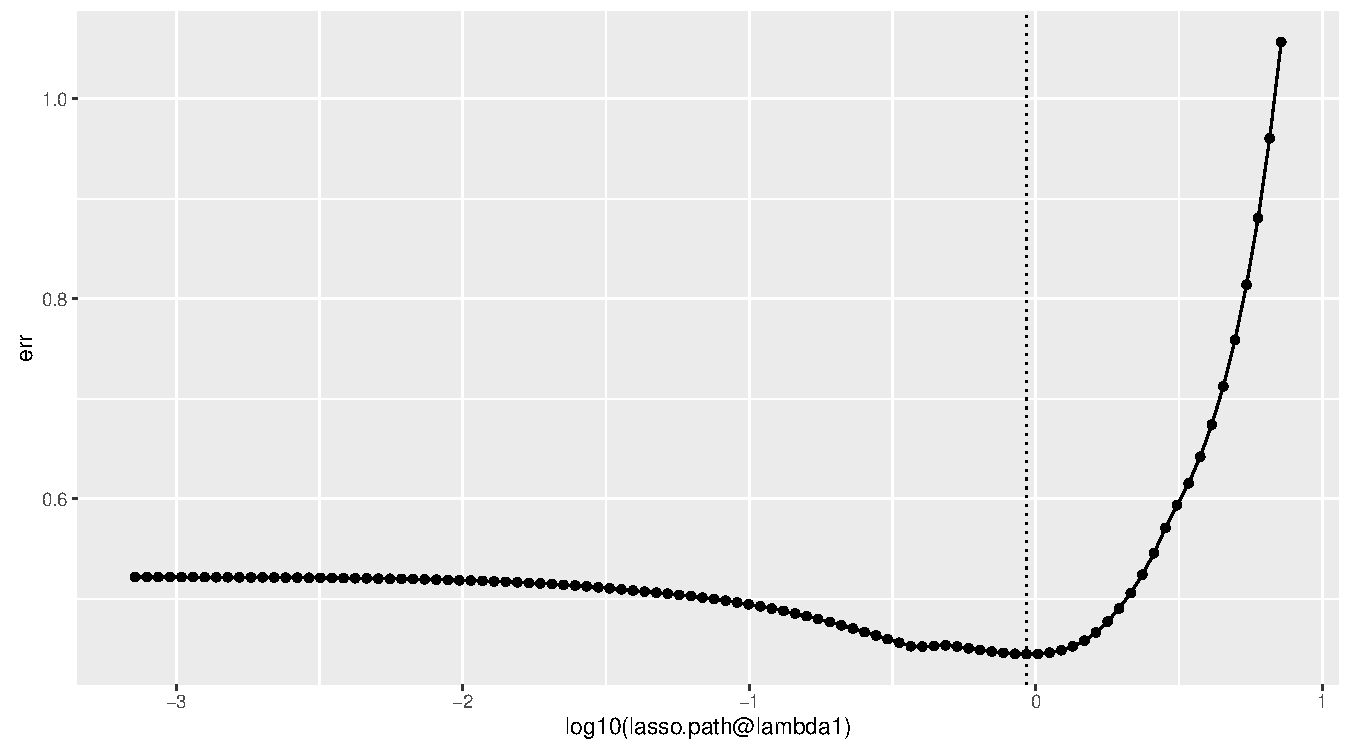
\includegraphics[width=\textwidth]{figures/lasso-unnamed-chunk-64-1} 

\end{knitrout}
\end{frame}

\begin{frame}[containsverbatim]
  \frametitle{Chemin de solution (en fonction de $\lambda$)}

\begin{knitrout}\scriptsize
\definecolor{shadecolor}{rgb}{0.969, 0.969, 0.969}\color{fgcolor}\begin{kframe}
\begin{alltt}
\hlkwd{plot}\hlstd{(lasso.path,} \hlkwc{labels}\hlstd{=}\hlkwd{colnames}\hlstd{(x.train),} \hlkwc{log.scale}\hlstd{=}\hlnum{FALSE}\hlstd{)}
\end{alltt}
\end{kframe}
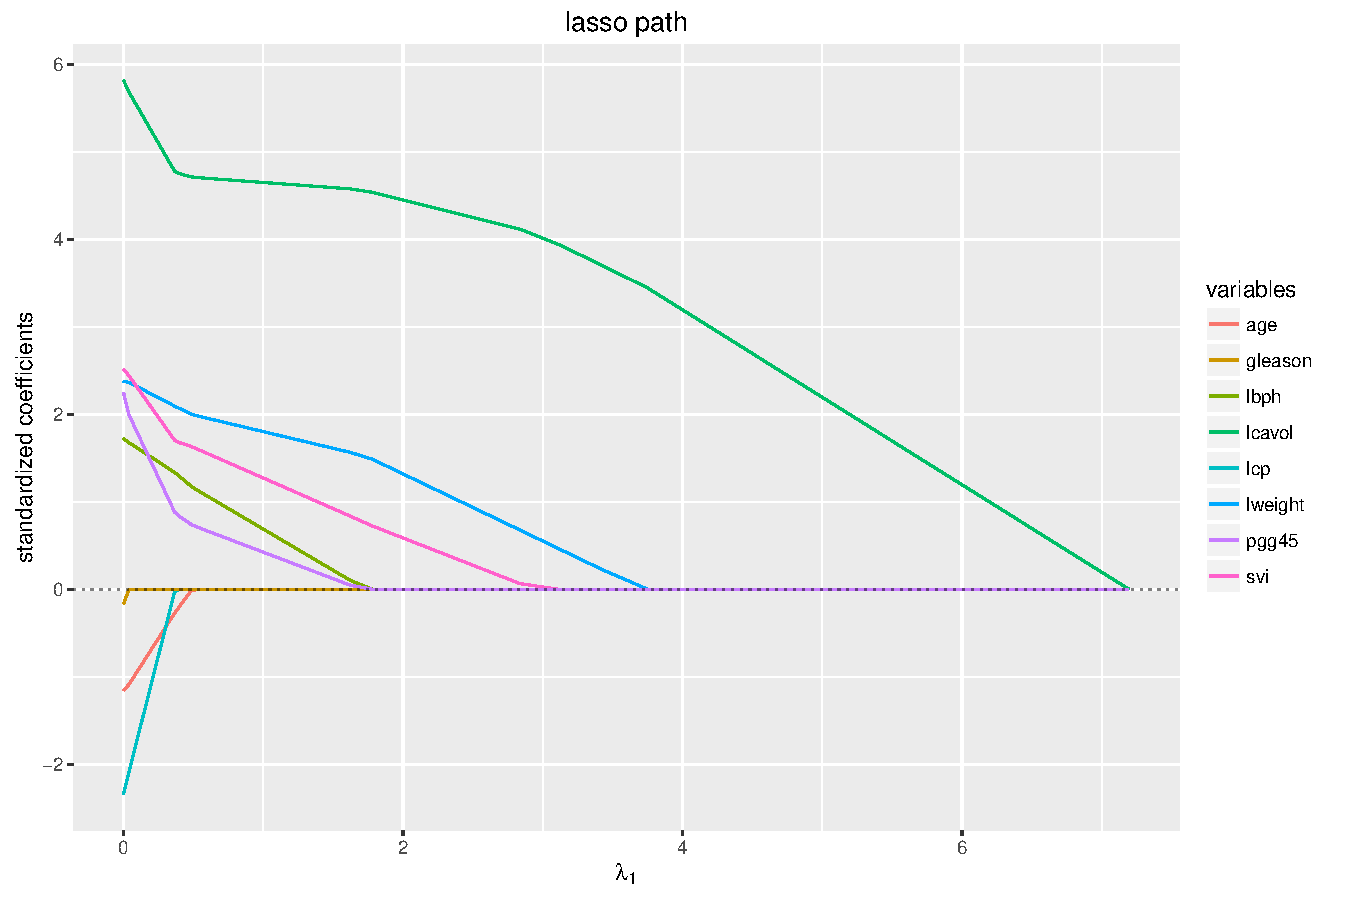
\includegraphics[width=\textwidth]{figures/lasso-unnamed-chunk-65-1} 

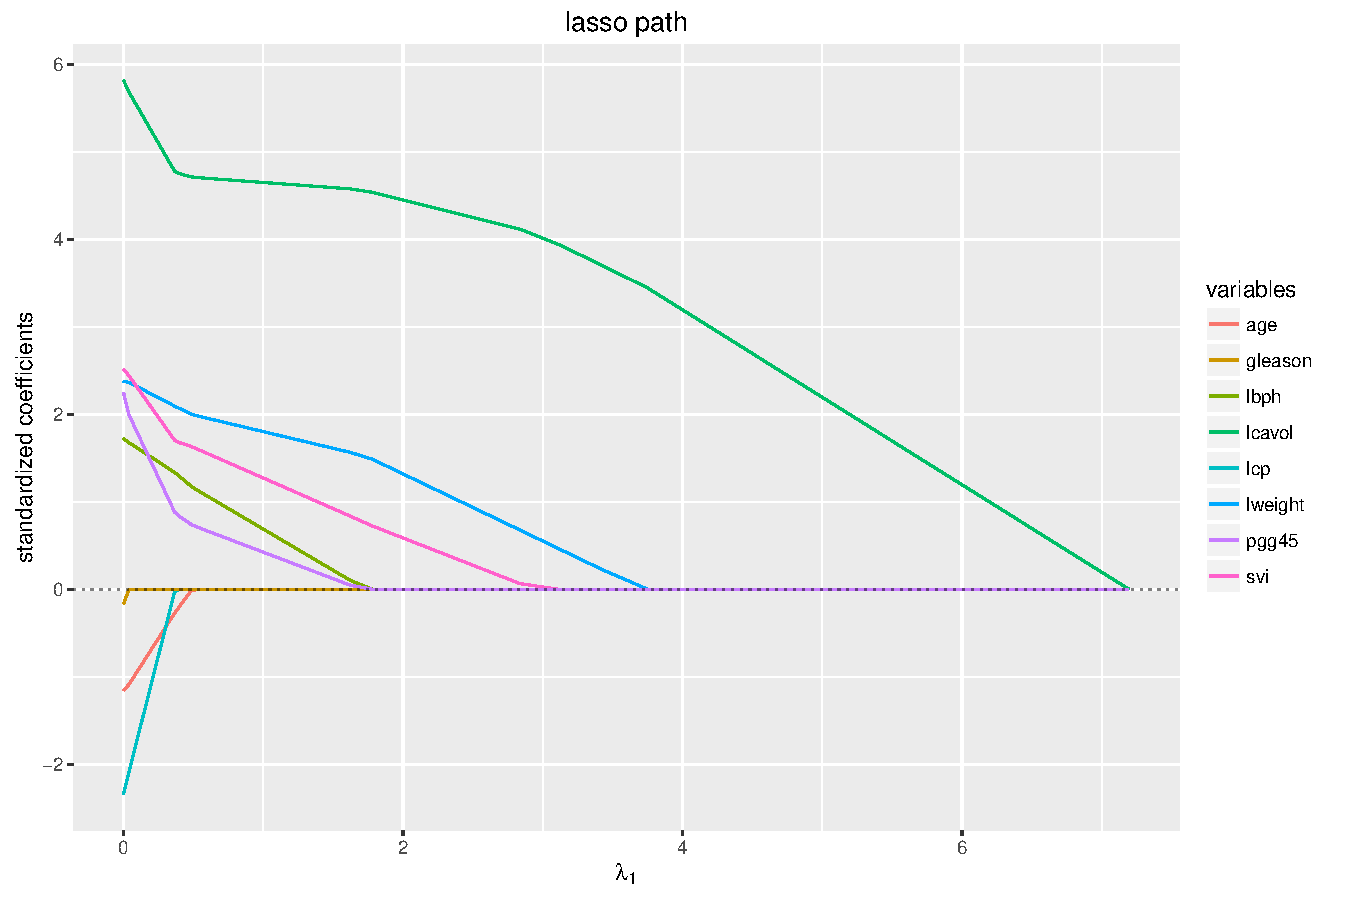
\includegraphics[width=\textwidth]{figures/lasso-unnamed-chunk-65-2} 

\end{knitrout}
\end{frame}

\begin{frame}[containsverbatim]
  \frametitle{Chemin de solution (en fonction de $log_{10}(\lambda)$)}

\begin{knitrout}\scriptsize
\definecolor{shadecolor}{rgb}{0.969, 0.969, 0.969}\color{fgcolor}\begin{kframe}
\begin{alltt}
\hlkwd{plot}\hlstd{(lasso.path,} \hlkwc{labels}\hlstd{=}\hlkwd{colnames}\hlstd{(x.train))}
\end{alltt}
\end{kframe}
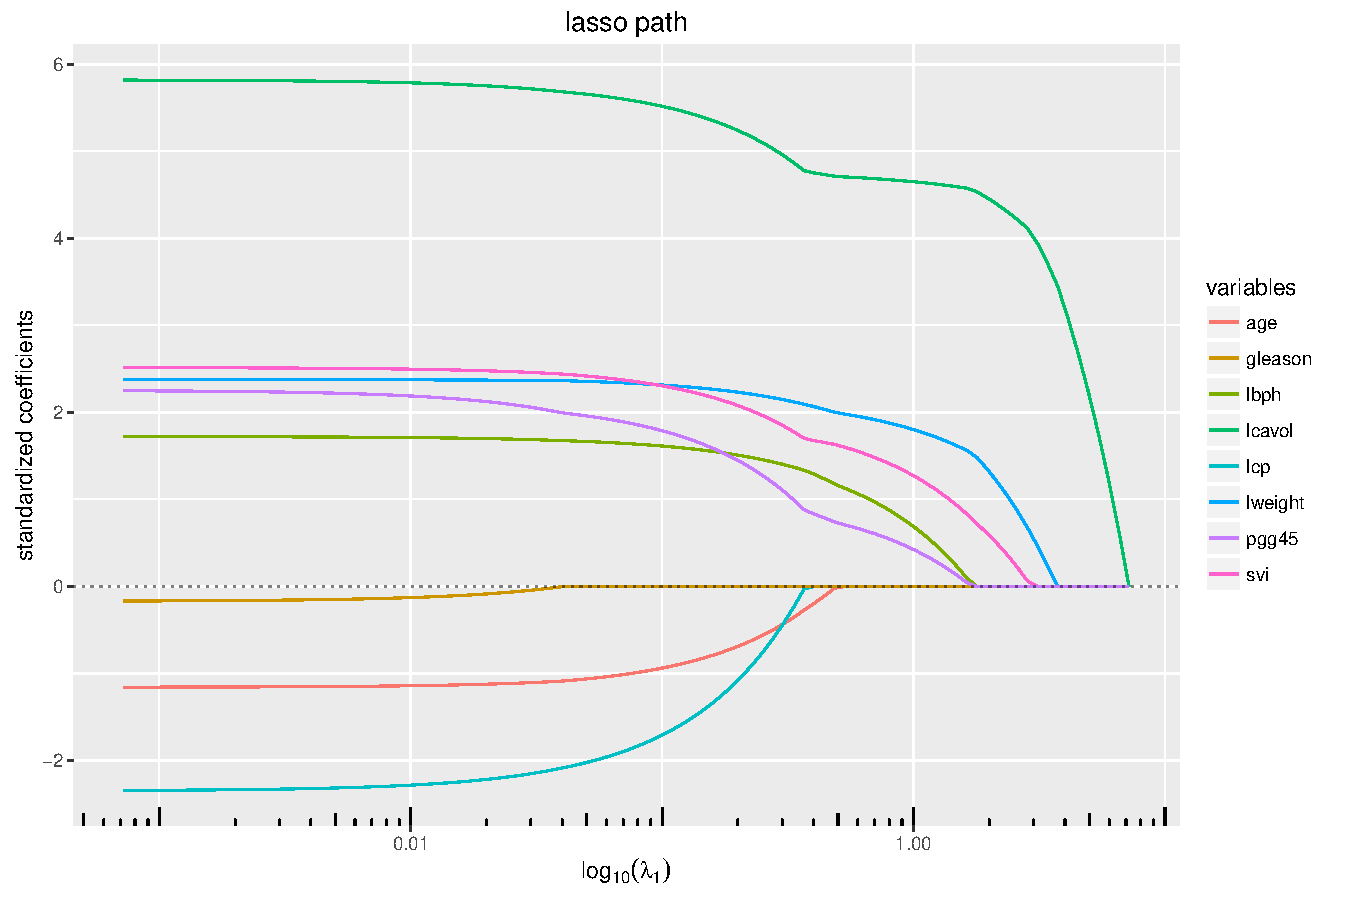
\includegraphics[width=\textwidth]{figures/lasso-unnamed-chunk-66-1} 

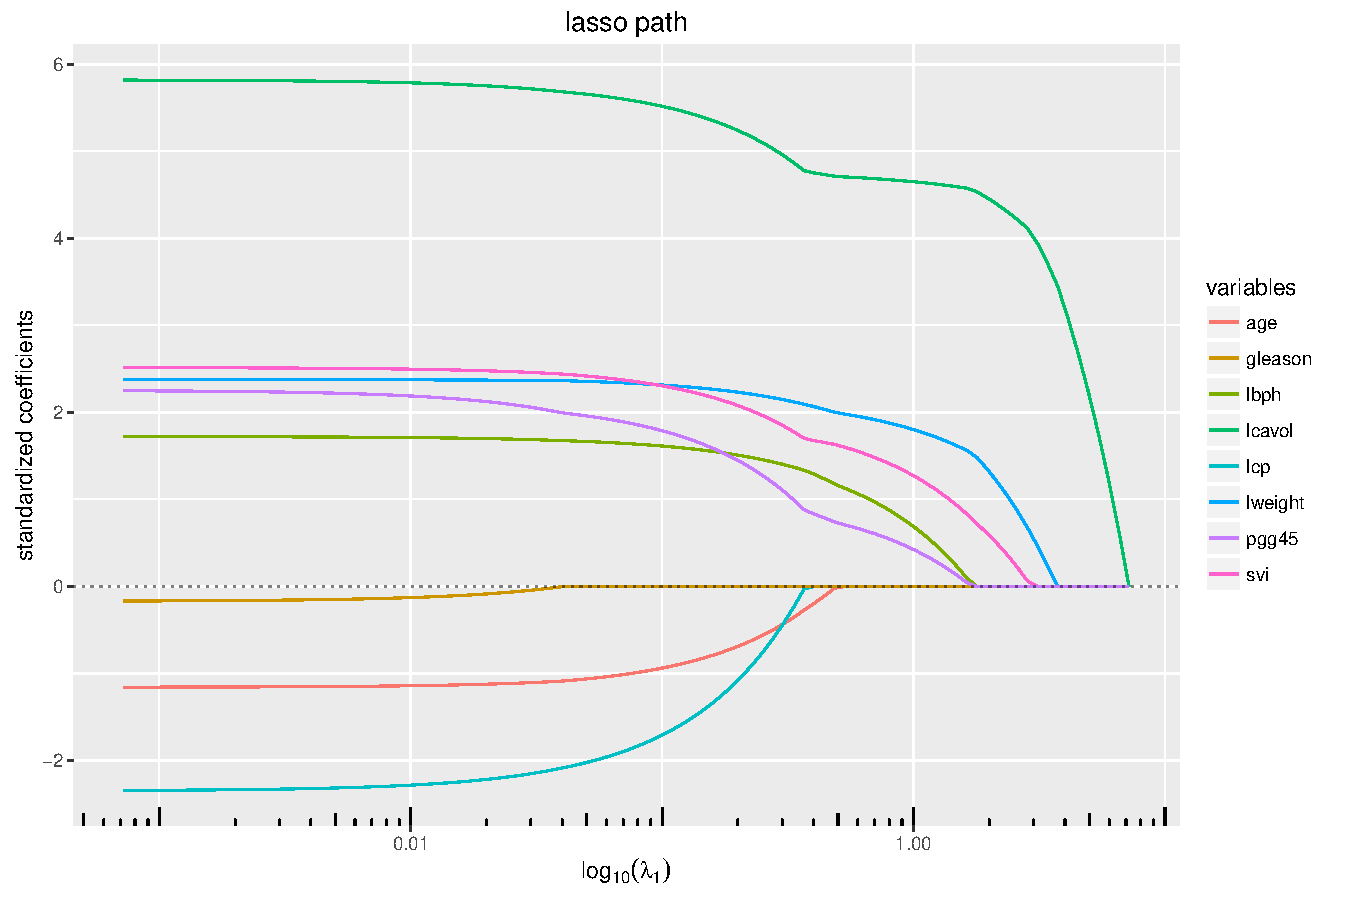
\includegraphics[width=\textwidth]{figures/lasso-unnamed-chunk-66-2} 

\end{knitrout}
\end{frame}

\begin{frame}[containsverbatim]
  \frametitle{Chemin de solution (proportion de régularisation $s$)}

\begin{knitrout}\scriptsize
\definecolor{shadecolor}{rgb}{0.969, 0.969, 0.969}\color{fgcolor}\begin{kframe}
\begin{alltt}
\hlkwd{plot}\hlstd{(lasso.path,} \hlkwc{labels}\hlstd{=}\hlkwd{colnames}\hlstd{(x.train),} \hlkwc{xvar}\hlstd{=}\hlstr{"fraction"}\hlstd{)}
\end{alltt}
\end{kframe}
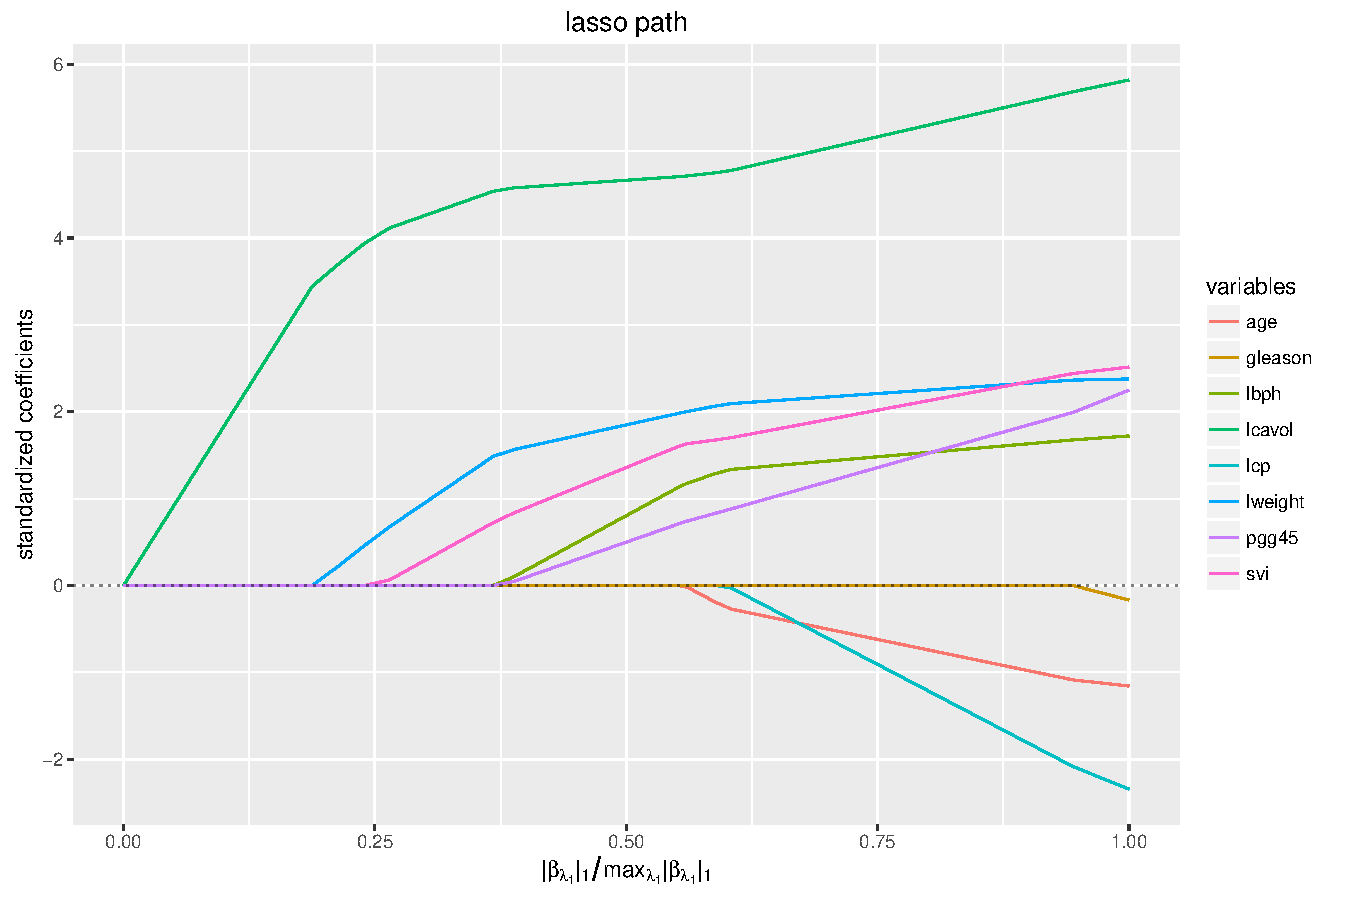
\includegraphics[width=\textwidth]{figures/lasso-unnamed-chunk-67-1} 

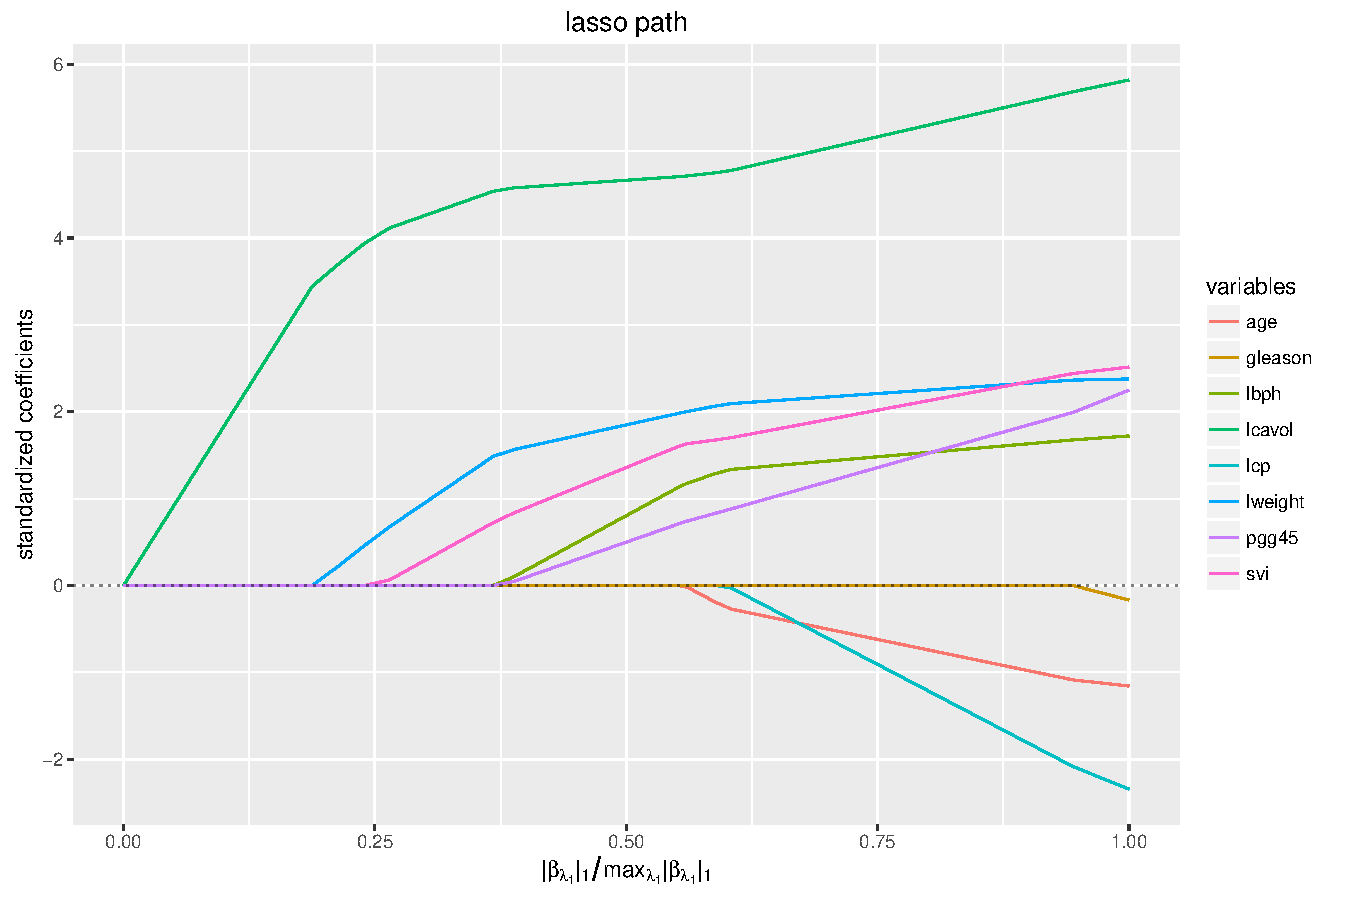
\includegraphics[width=\textwidth]{figures/lasso-unnamed-chunk-67-2} 

\end{knitrout}
\end{frame}

\subsubsection{Choix du paramètre de régularisation}

\begin{frame}
  \frametitle{Critères pénalisés}

  \begin{block}{Degrés de liberté du LASSO}
    On peut montrer que c'est simplement le nombre de prédicteurs actifs
\[
\mathrm{df}(\hat{\by}_\lambda^{\text{lasso}}) = \mathrm{card}(\set{j:\beta_j(\lambda)\neq 0}) = |\mathcal{A}|.
\]
  \end{block}

  \begin{itemize}
 % \item  \alert{Mallows'  $C_p$} , défini lorsque $\hat{\sigma}$ est sans biais
 %     \begin{equation*}
 %       C_p = \mathrm{err}_{\mathcal{D}} +2 \frac{|\mathcal{A}|}{n} \hat{\sigma}^2.
 %     \end{equation*}
    \item \alert{Akaike Information Criterion} équivalent au  $C_p$ en régression
        \begin{equation*}
          \mathrm{AIC} = -2 \mathrm{loglik} + 2\frac{|\mathcal{A}|}{n},
        \end{equation*}
      \item \alert{Bayesian   Information   Criterion}
        \begin{equation*}
          \mathrm{BIC} = -2\mathrm{loglik} + |\mathcal{A}|\log(n),
        \end{equation*}
      \item \alert{modified BIC} (lorsque $n < p$)
        \begin{equation*}
          \mathrm{mBIC} = -2\mathrm{loglik} + |\mathcal{A}|\log(p),
        \end{equation*}
      \item \alert{Extended BIC} ajoute un prior sur le nombre de modèles de taille  $|\mathcal{A}|$
        \begin{equation*}
          \mathrm{eBIC} = -2\mathrm{loglik} + |\mathcal{A}|(\log(n) + 2\log(p)).
        \end{equation*}
      \end{itemize}
\end{frame}






\begin{frame}[containsverbatim]
  \frametitle{Cancer de la prostate}
  \framesubtitle{Calcul de l' AIC/BIC en estimant $\sigma$}

\begin{knitrout}\scriptsize
\definecolor{shadecolor}{rgb}{0.969, 0.969, 0.969}\color{fgcolor}\begin{kframe}
\begin{alltt}
\hlstd{crit} \hlkwb{<-} \hlkwd{criteria}\hlstd{(lasso.path,} \hlkwc{plot}\hlstd{=}\hlnum{FALSE}\hlstd{)}
\hlkwd{print}\hlstd{(}\hlkwd{head}\hlstd{(crit}\hlopt{$}\hlstd{criterion),} \hlkwc{digits}\hlstd{=}\hlnum{3}\hlstd{)}
\end{alltt}
\begin{verbatim}
##    AIC  BIC    GCV df lambda fraction
## 1 4.60 4.60 0.0208  1   7.19   0.0000
## 2 4.53 4.53 0.0184  2   6.55   0.0192
## 3 4.44 4.45 0.0168  2   5.97   0.0367
## 4 4.37 4.37 0.0156  2   5.44   0.0527
## 5 4.30 4.30 0.0145  2   4.96   0.0672
## 6 4.23 4.24 0.0136  2   4.52   0.0805
\end{verbatim}
\begin{alltt}
\hlkwd{print}\hlstd{(}\hlkwd{head}\hlstd{(crit}\hlopt{$}\hlstd{beta.min))}
\end{alltt}
\begin{verbatim}
## 6 x 2 sparse Matrix of class "dgCMatrix"
##                AIC        BIC
## lcavol   1.0203631  1.0203631
## lweight  2.2474028  2.2474028
## age     -1.1631499 -1.1631499
## lbph     0.2061171  0.2061171
## svi      0.3400045  0.3400045
## lcp     -0.2573030 -0.2573030
\end{verbatim}
\end{kframe}
\end{knitrout}
\end{frame}



\begin{frame}[containsverbatim]
  \frametitle{Cancer de la prostate}
  \framesubtitle{Calcul de l' AIC/BIC en estimant $\sigma$ (plot)}

\begin{knitrout}\scriptsize
\definecolor{shadecolor}{rgb}{0.969, 0.969, 0.969}\color{fgcolor}
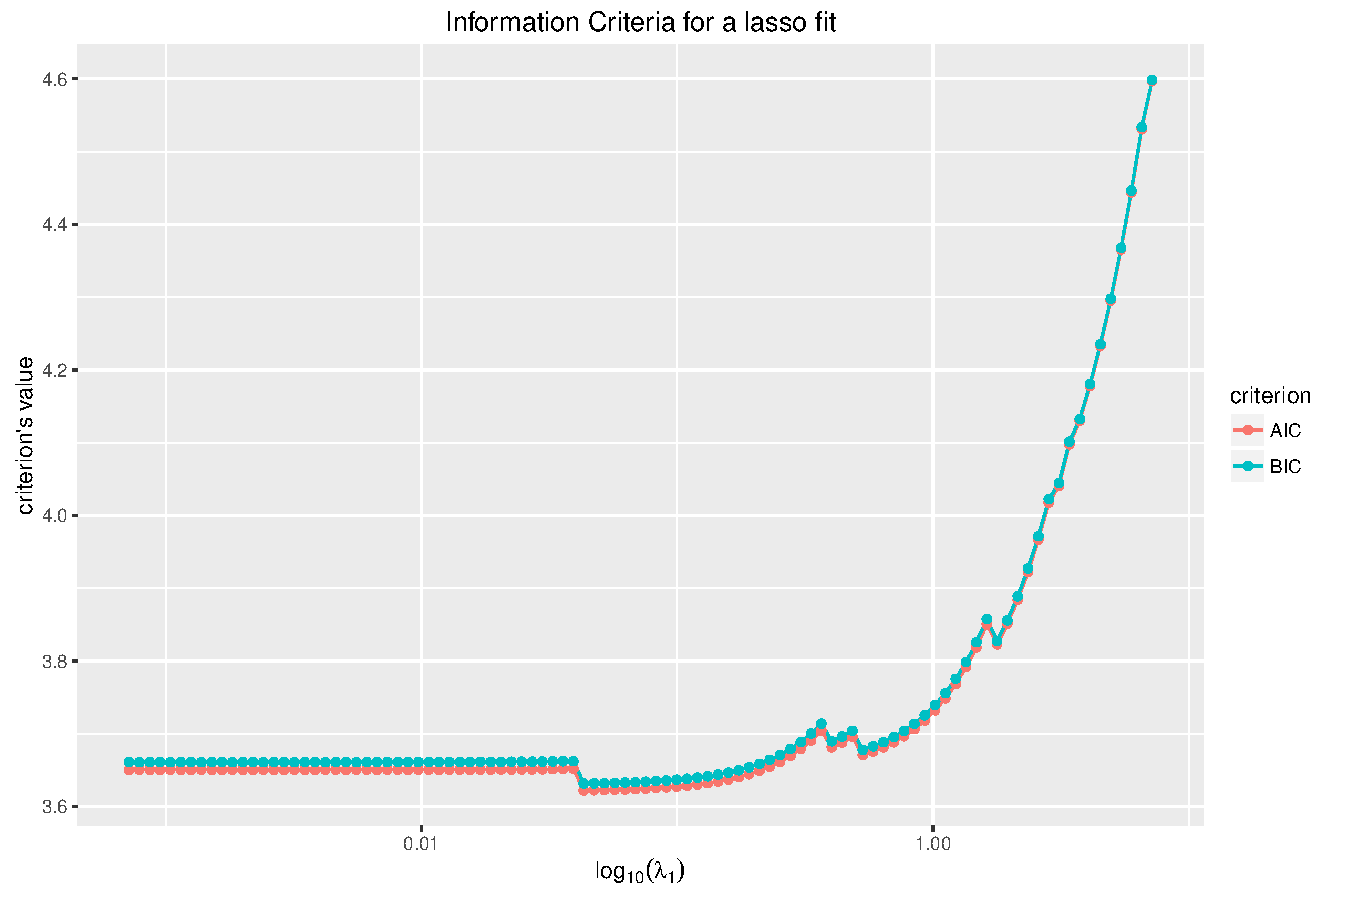
\includegraphics[width=\textwidth]{figures/crit_lassounnamed-chunk-70-1} 

\end{knitrout}
\end{frame}

\begin{frame}[containsverbatim]
  \frametitle{Cancer de la prostate}
  \framesubtitle{Calcul de l' AIC/BIC en estimant $\sigma$ (plot 2)}

\begin{knitrout}\scriptsize
\definecolor{shadecolor}{rgb}{0.969, 0.969, 0.969}\color{fgcolor}
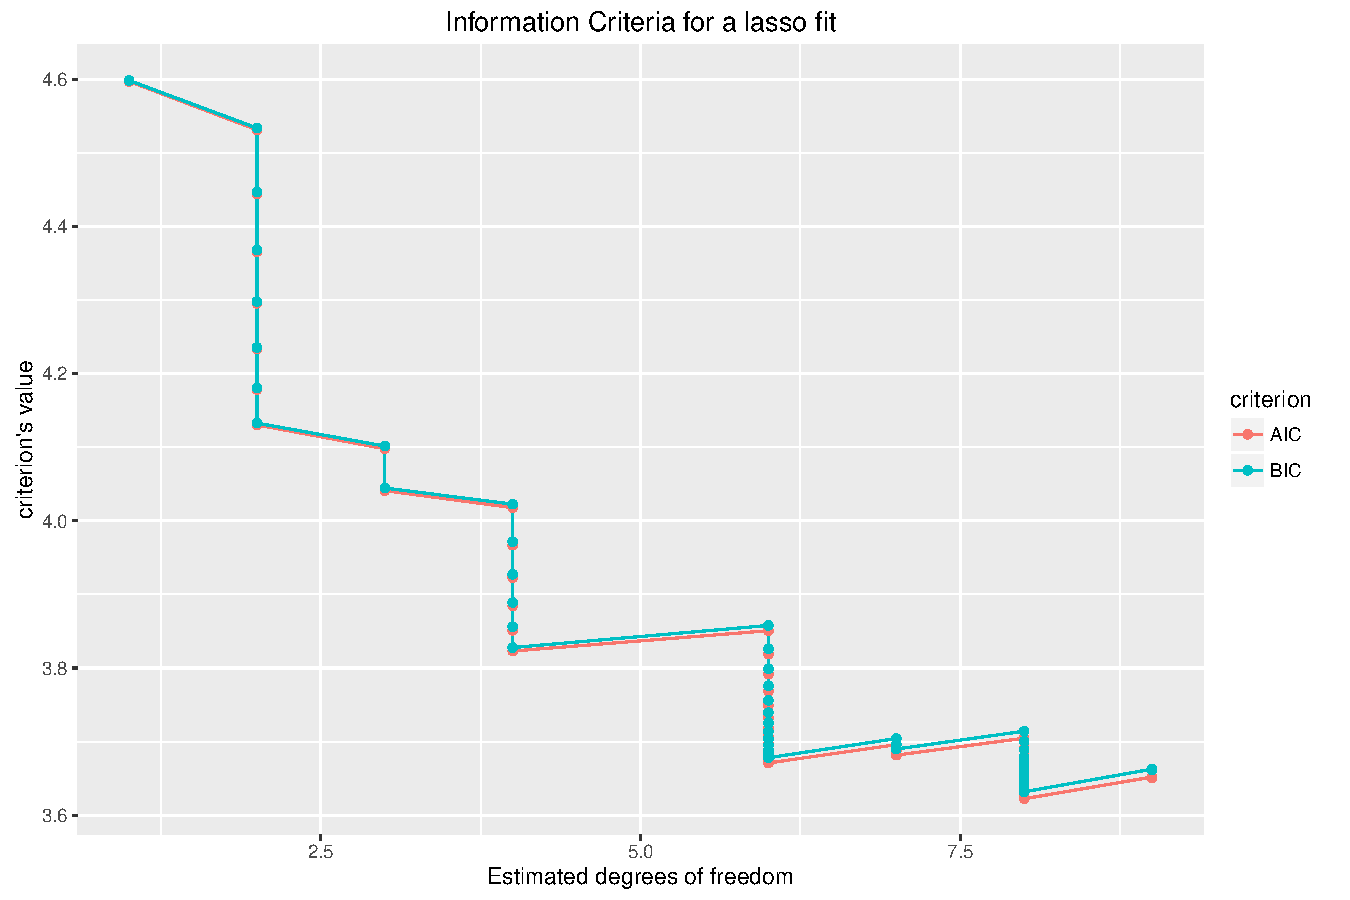
\includegraphics[width=\textwidth]{figures/crit_lassounnamed-chunk-71-1} 

\end{knitrout}
\end{frame}


\begin{frame}[containsverbatim]
  \frametitle{Validation croisée}

  La validation croisée se parallèlise facilement et ne prend que peu de temps sur un petit jeu de données

\begin{knitrout}\scriptsize
\definecolor{shadecolor}{rgb}{0.969, 0.969, 0.969}\color{fgcolor}\begin{kframe}
\begin{alltt}
\hlkwd{system.time}\hlstd{(loo} \hlkwb{<-} \hlkwd{crossval}\hlstd{(x.train,y.train,}\hlstr{"lasso"}\hlstd{,}\hlkwc{K}\hlstd{=n,}\hlkwc{normalize}\hlstd{=}\hlnum{FALSE}\hlstd{))}
\end{alltt}
\begin{verbatim}
## 
## CROSS-VALIDATION FOR  lasso  REGULARIZER 
## 
## 67-fold CV on the lambda1 grid, lambda2 is fixed.
##    user  system elapsed 
##   0.724   0.236   0.343
\end{verbatim}
\end{kframe}
\end{knitrout}

\begin{knitrout}\scriptsize
\definecolor{shadecolor}{rgb}{0.969, 0.969, 0.969}\color{fgcolor}\begin{kframe}
\begin{alltt}
\hlkwd{system.time}\hlstd{(CV10} \hlkwb{<-} \hlkwd{crossval}\hlstd{(x.train,y.train,}\hlstr{"lasso"}\hlstd{,}\hlkwc{K}\hlstd{=}\hlnum{10}\hlstd{,}\hlkwc{normalize}\hlstd{=}\hlnum{FALSE}\hlstd{))}
\end{alltt}
\begin{verbatim}
## 
## CROSS-VALIDATION FOR  lasso  REGULARIZER 
## 
## 10-fold CV on the lambda1 grid, lambda2 is fixed.
##    user  system elapsed 
##   0.472   0.632   0.258
\end{verbatim}
\end{kframe}
\end{knitrout}

\end{frame}

\begin{frame}[containsverbatim]
  \frametitle{Validation croisée ("leave one out")}
\begin{knitrout}\scriptsize
\definecolor{shadecolor}{rgb}{0.969, 0.969, 0.969}\color{fgcolor}
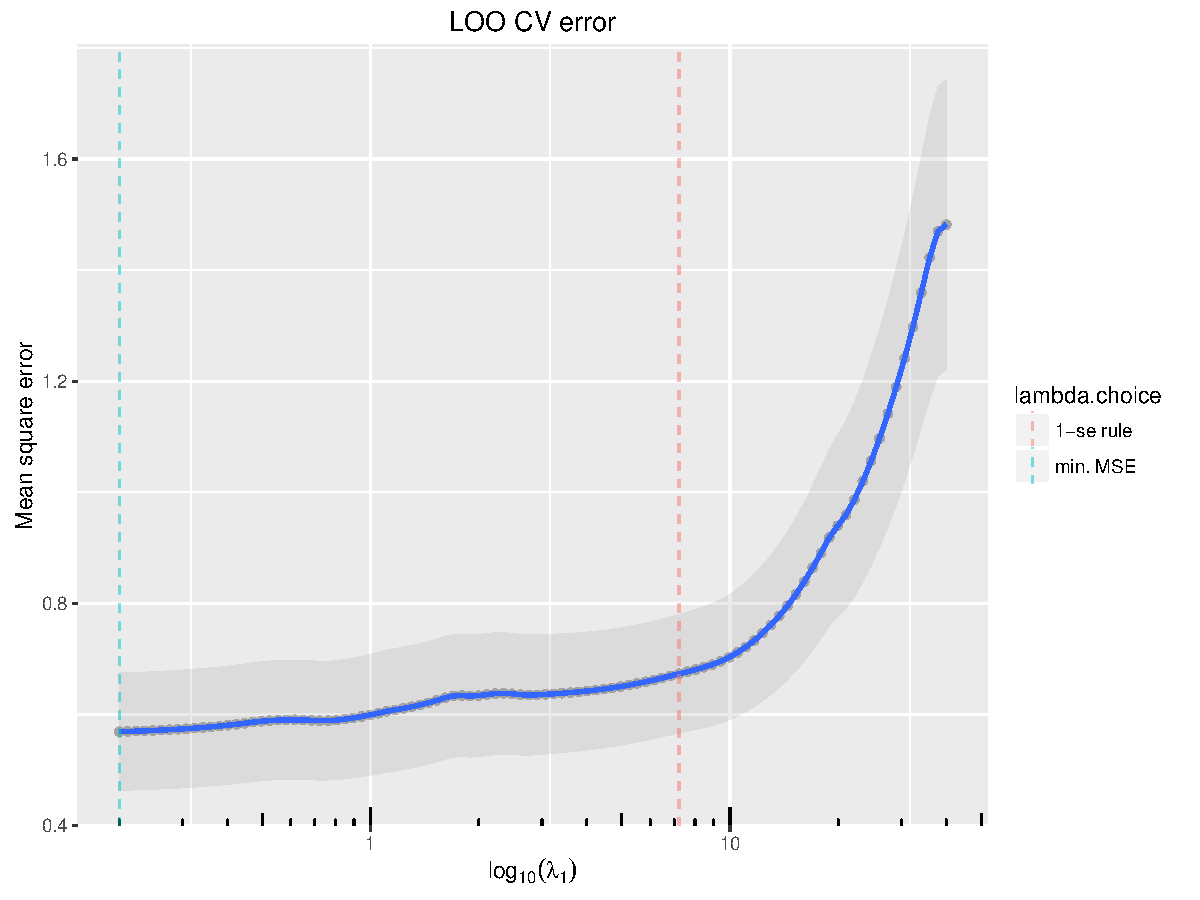
\includegraphics[width=\textwidth]{figures/crit_lassounnamed-chunk-74-1} 

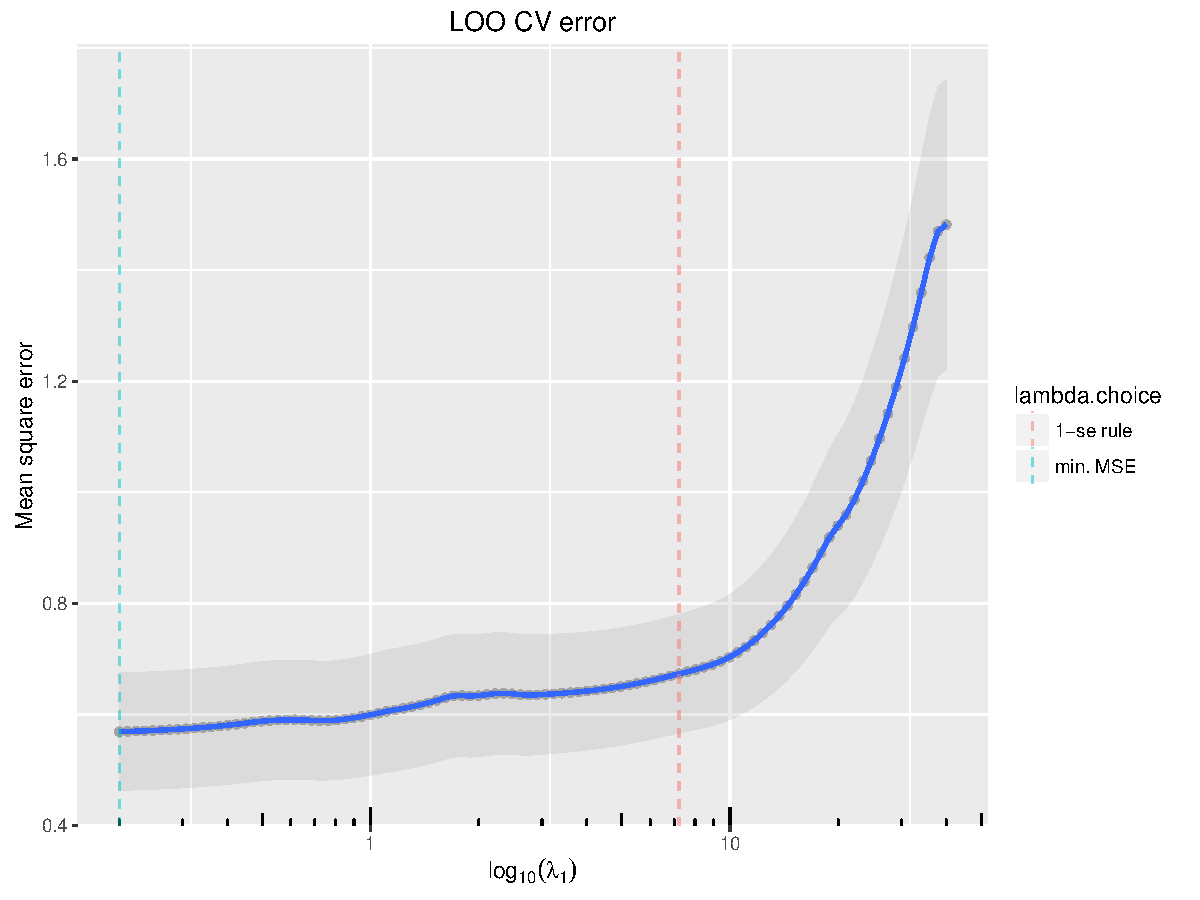
\includegraphics[width=\textwidth]{figures/crit_lassounnamed-chunk-74-2} 

\end{knitrout}
\end{frame}



\begin{frame}[containsverbatim]
  \frametitle{Validation croisée ("ten fold")}
\begin{knitrout}\scriptsize
\definecolor{shadecolor}{rgb}{0.969, 0.969, 0.969}\color{fgcolor}
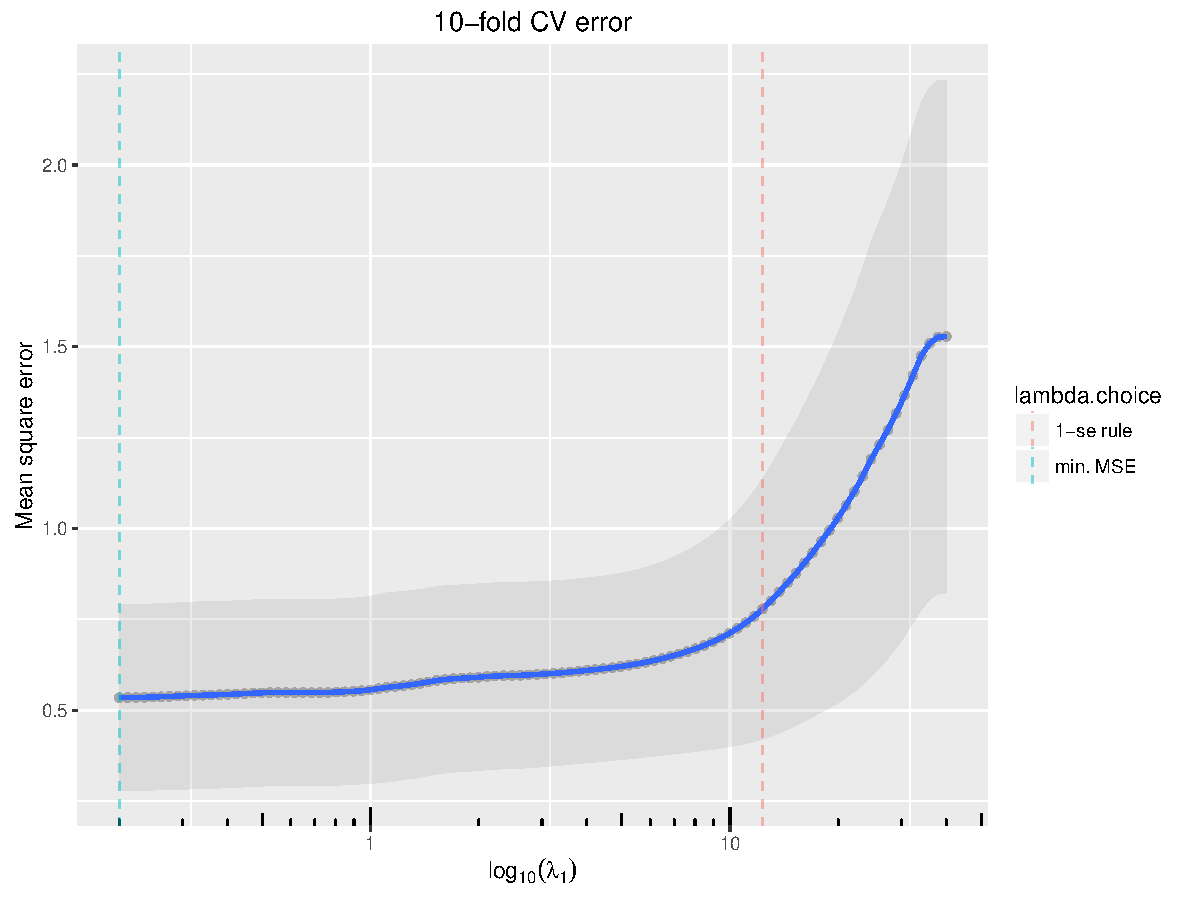
\includegraphics[width=\textwidth]{figures/crit_lassounnamed-chunk-75-1} 

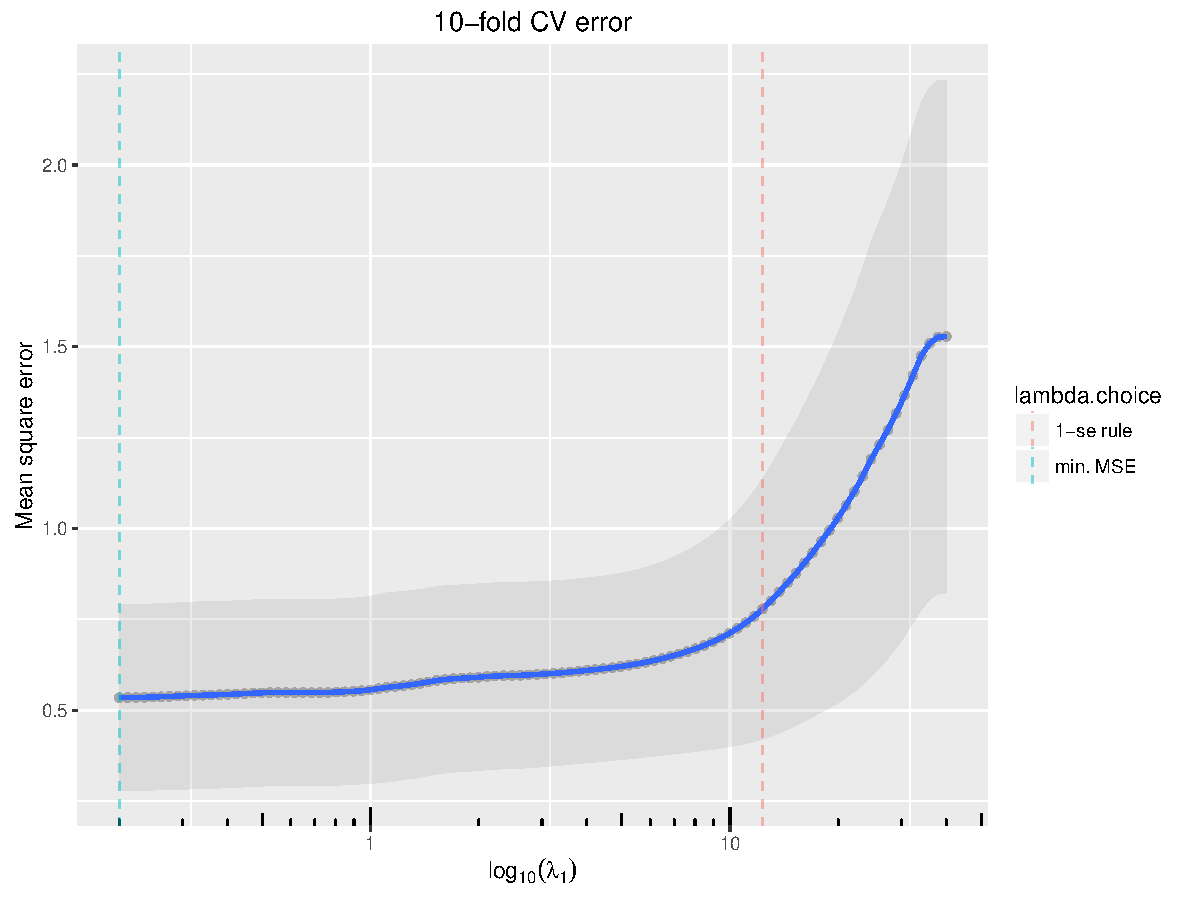
\includegraphics[width=\textwidth]{figures/crit_lassounnamed-chunk-75-2} 

\end{knitrout}
\end{frame}






\subsection{Variations autour du Lasso}

\begin{frame}{Bridge regression}
  
  \begin{block}{A simple interpretable model: Gaussian linear regression}
    Assume  a   linear  relationship  between  the   features  $\bX  =
    (\bx_1,\dots,\bx_p)$ and the outcome $\by = (y_1,\dots, y_n)$ plus
    an \emph{iid} Gaussian noise:
    \begin{displaymath}
      \by = \mu \I_n + \bX \bbeta^\star + \bvarepsilon, \qquad \bvarepsilon\sim\mathcal{N}(\bzr_n, \sigma^2\bI_n). 
    \end{displaymath}        

  \end{block}

  \only<2>{
    \begin{itemize}
    \item OLS would fail in the $n<p$ setup or in presence of highly
      correlated features
    \item Bridge regression regularizes by controlling the size of the
      coefficients
    \end{itemize}
  }
  
  \begin{block}{The bridge estimator}<3-> Force $\hatbbeta$ to live in
    balls associated with the $\ell_\gamma$-norms:
    \begin{equation*}
      \hatbbeta_{\lambda,\gamma} = \argmin_{\bbeta\in\Rset^p}
      \frac{1}{2} \|\by - \bX \beta \|^2_2 \quad \text{such that} \quad \left\| \bbeta
      \right\|_\gamma^\gamma \leq c              
    \end{equation*}
    \onslide<4>{The Lagrangian form is
      \begin{equation*}
        \hatbbeta_{\lambda,\gamma} = \argmin_{\bbeta\in\Rset^p}
        \frac{1}{2} \|\by - \bX \beta \|^2_2 +  \lambda \left\|  \bbeta \right\|_\gamma^\gamma.
      \end{equation*}
    }
  \end{block}

\end{frame}

\begin{frame}{Bridge regression}

  \begin{figure}[htbp!]
    \centering
    \begin{tabular}{ccc}
      $\ell_0$ & $\ell_{1/3}$ & $\ell_{1/2}$ \\
      
\includegraphics[width=.125\textwidth]{figures/ell0ball}
      & 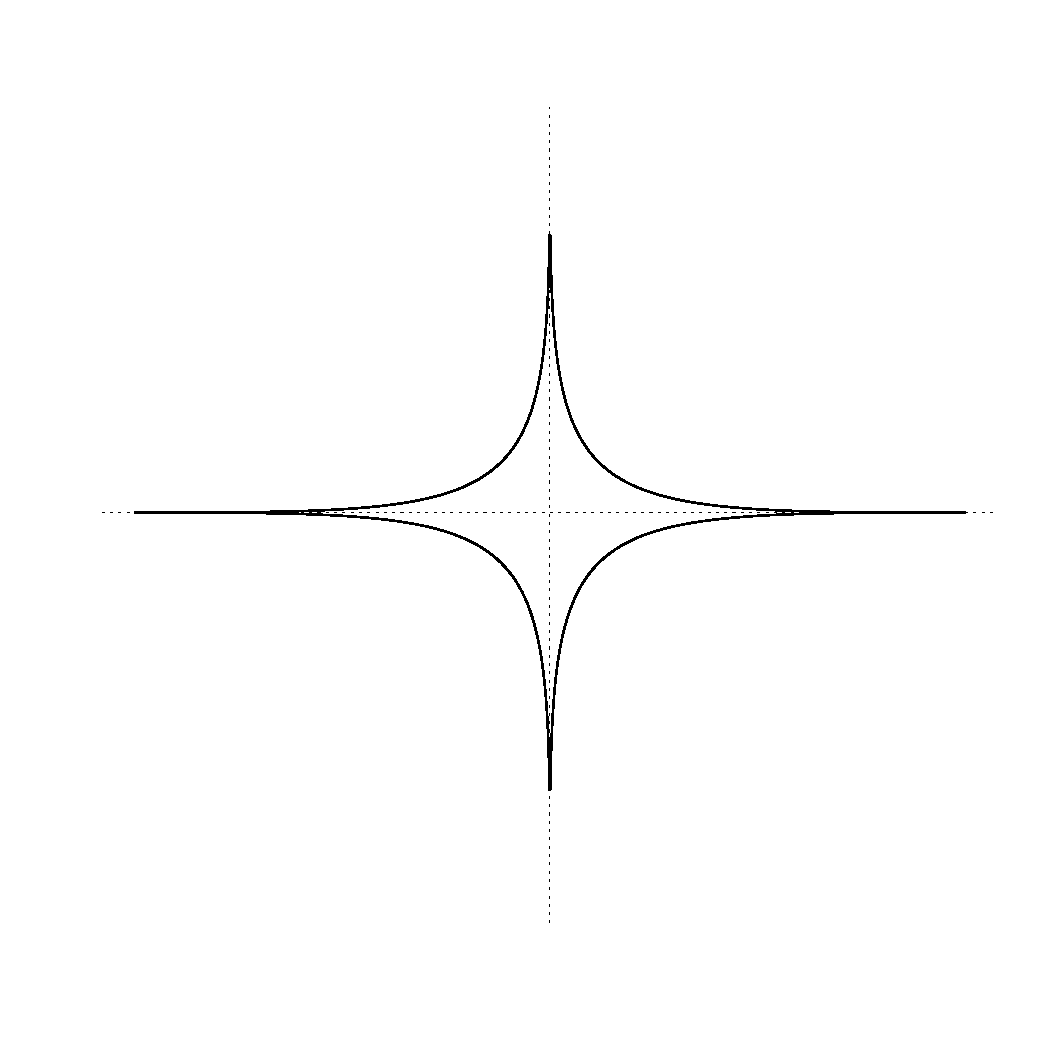
\includegraphics[width=.125\textwidth]{figures/ell13ball}
      & 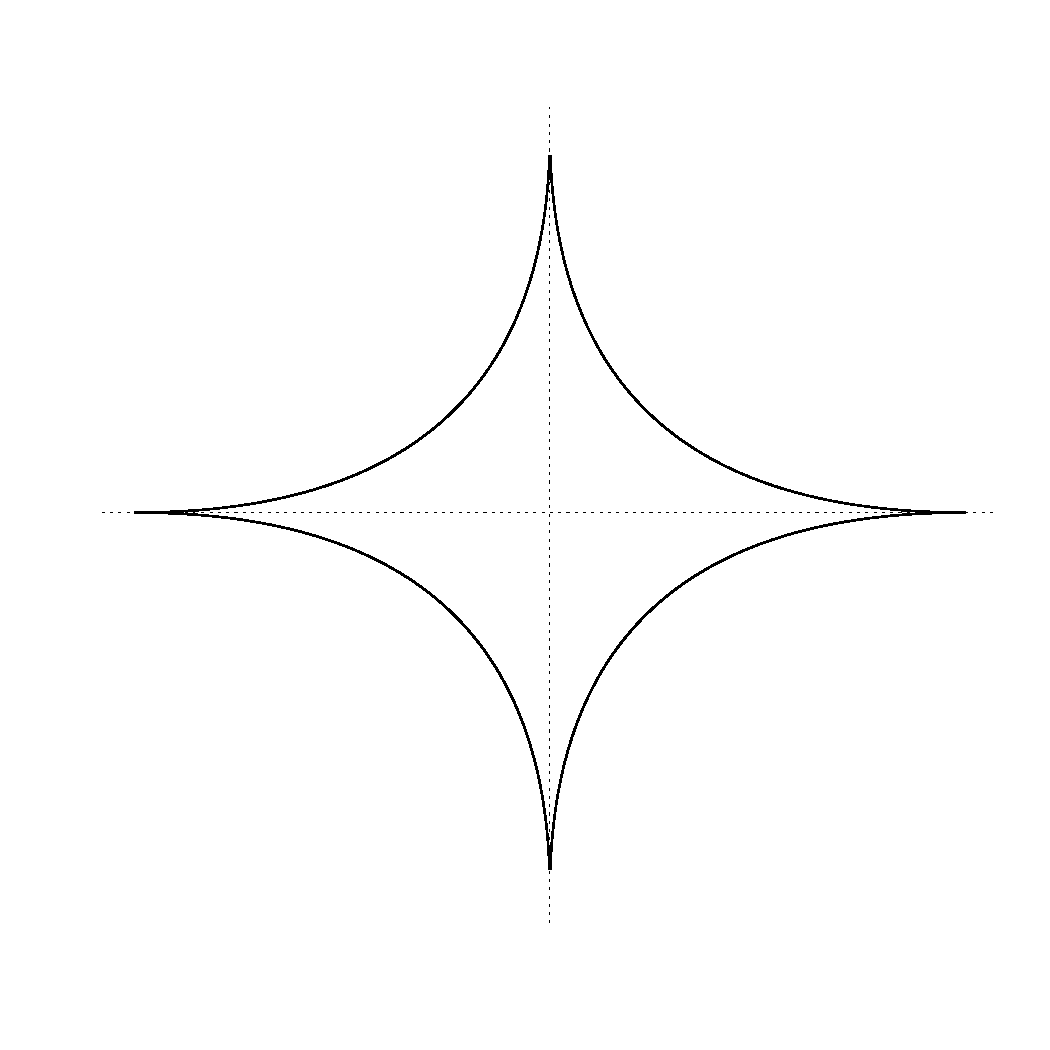
\includegraphics[width=.125\textwidth]{figures/ell12ball} \\
      \multicolumn{3}{c}{$\ell_1$} \\
      \multicolumn{3}{c}{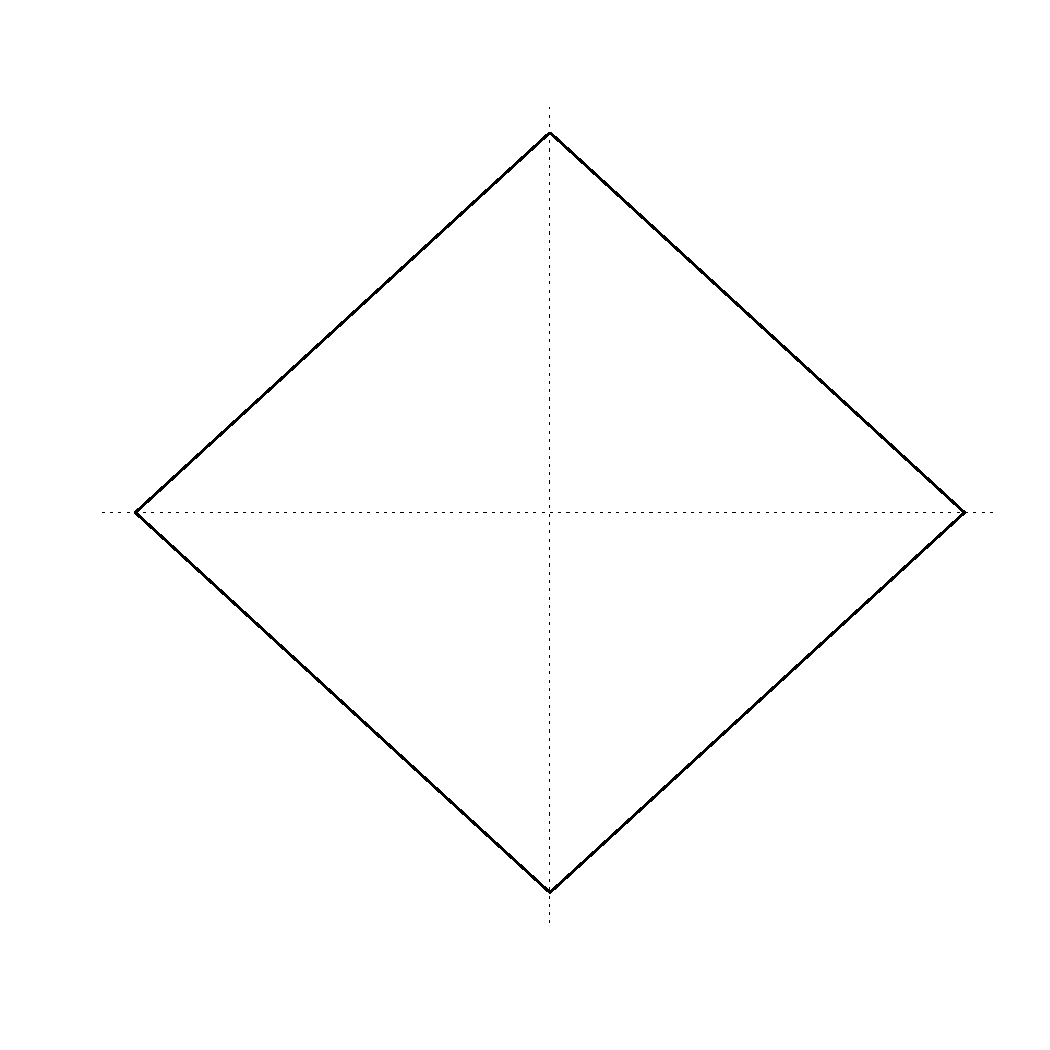
\includegraphics[width=.125\textwidth]{figures/ell1ball}} \\
      $\ell_2$ & $\ell_3$ & $\ell_\infty$ \\
      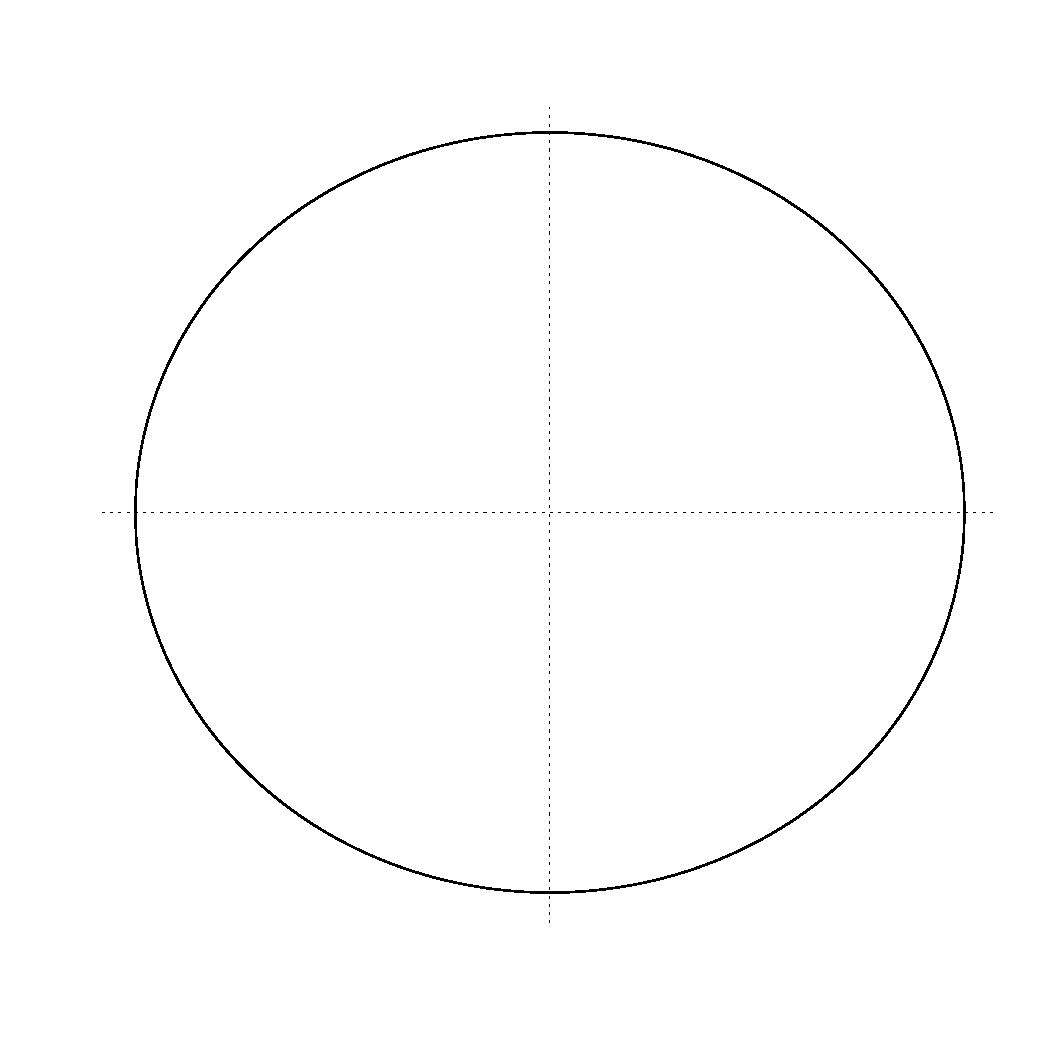
\includegraphics[width=.125\textwidth]{figures/ell2ball}
      & 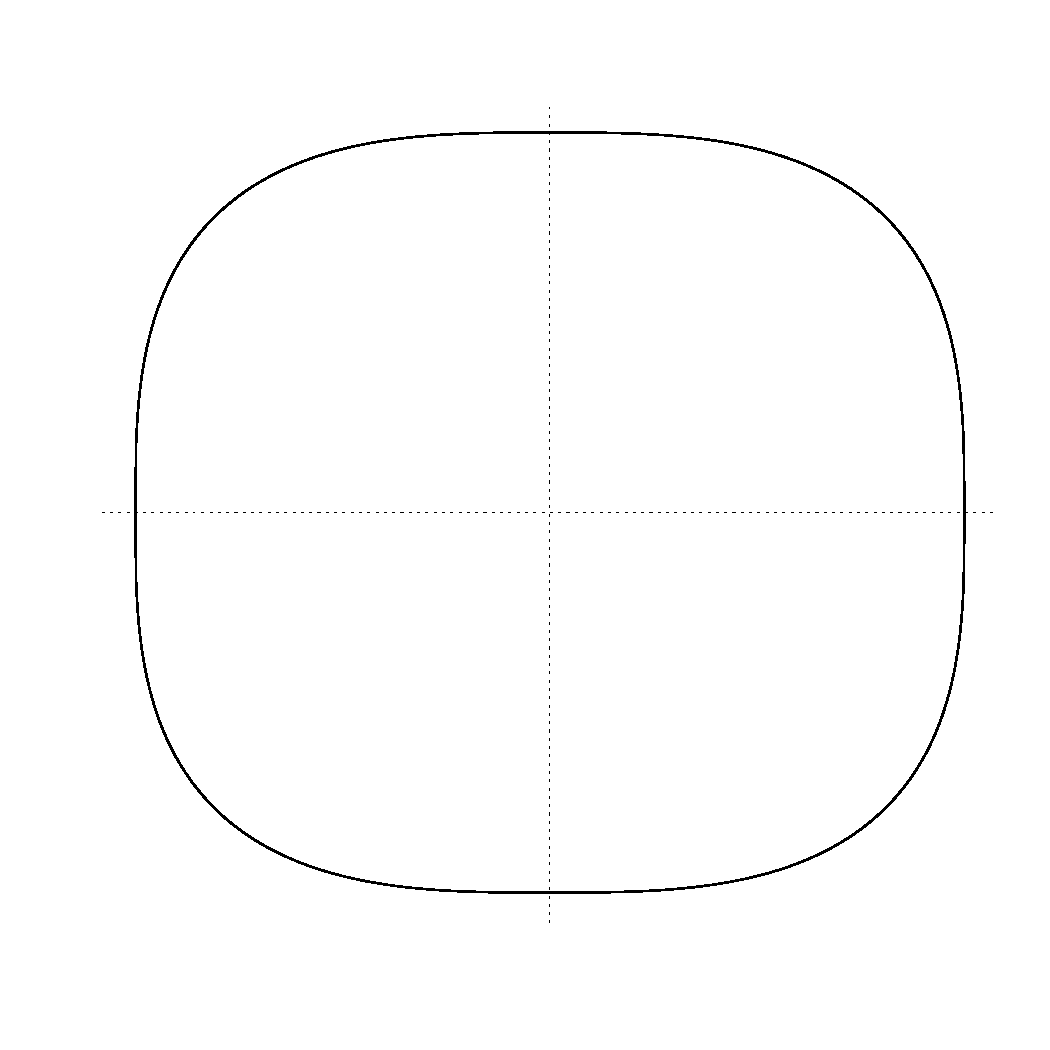
\includegraphics[width=.125\textwidth]{figures/ell3ball}
      & 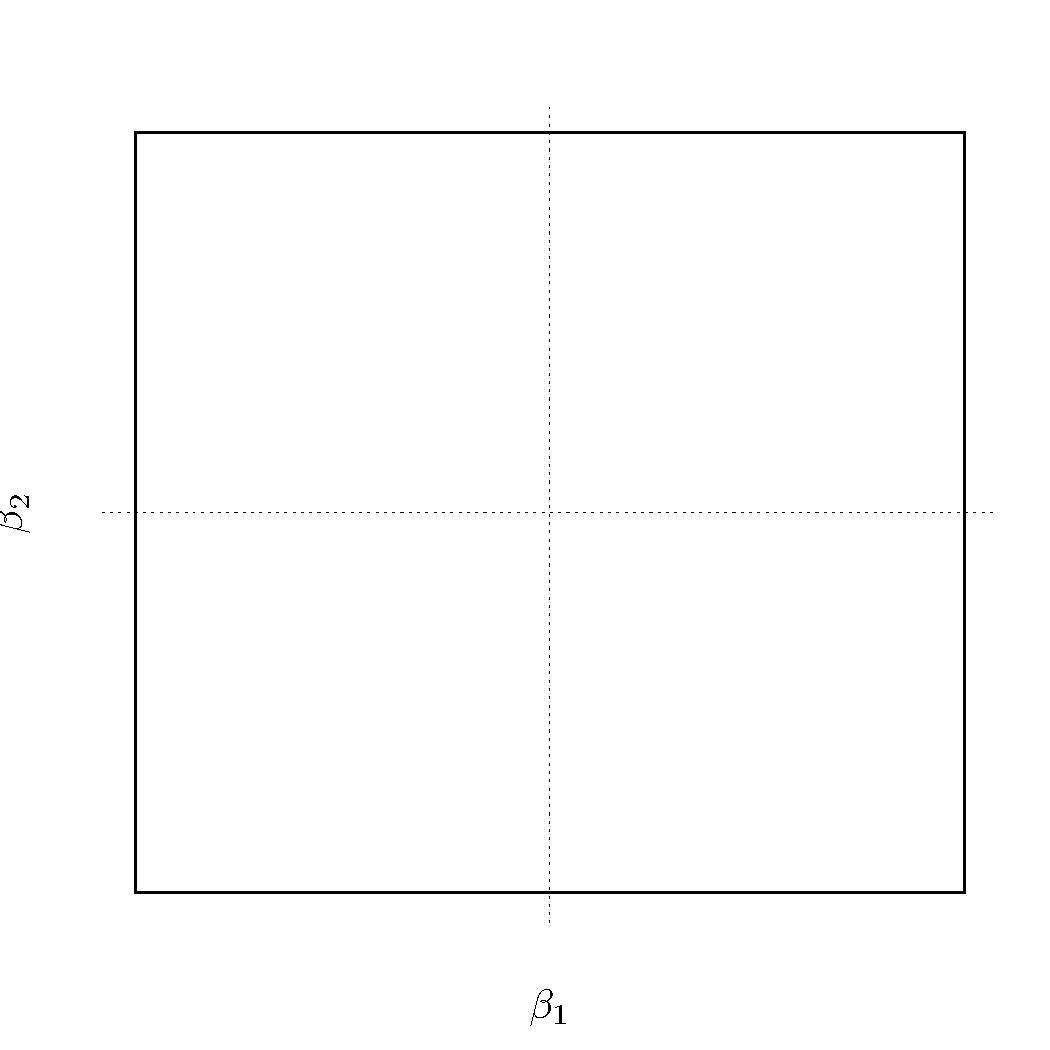
\includegraphics[width=.125\textwidth]{figures/ellinfball} \\
    \end{tabular}
    \caption{Contours of the feasible sets for various  $\gamma$ when $\bbeta\in\Rset^2$.}
    \label{fig:bridge_set}
  \end{figure}
  
\end{frame}


\begin{frame}{Numerical illustration}
  \framesubtitle{True model mimicking the block-wise structure between SNP for
    the predictors}

  \begin{block}{Dispatched the true parameters in 5 groups} 
    \vspace{-.75cm}
    \begin{small}
      \begin{equation*}
        \bbeta^\star = \left(\underbrace{0.25, \dots, 0.25}_{p/4 \text{ times}},
          \underbrace{1,\dots,1}_{p/8 \text{ times}},
          \underbrace{-0.25,\dots,-0.25}_{p/4 \text{ times}},
          \underbrace{-1,\dots,-1}_{p/8 \text{ times}},
          \underbrace{0.25, \dots, 0.25}_{p/4 \text{ times}}\right).
      \end{equation*}
    \end{small}
  \end{block}
  
  \begin{block}{Faithful    block-wise    pattern    between    the    predictors}
    We let $\bx_i \sim \mathcal{N}(\bzr_p, \bSigma)$ with
    \pgfdeclareimage[height=1.8cm]{struct_cov}{figures/bloc_cov}
    \begin{small}
      \begin{equation*}
        \bSigma \ = \ \parbox{2cm}{\pgfuseimage{struct_cov}} \ 
        \text{ with } \Sigma_{ij} =
        \begin{cases}
          1 & i = j,\\
          .25 & i,j \in \text{ blocks \{1,3,5\}}, \ i \neq j, \\
          .75 & i,j \in \text{ blocks \{2,4\}}, \ i \neq j, \\
          0 & \text{otherwise}.
        \end{cases}
      \end{equation*}
    \end{small}
  \end{block}

  + Variance $\sigma^2$ of the noise chosen to met $R^2\approx 0.8$ on
  the training set.
  
\end{frame}

\begin{frame}{Numerical illustration}
  \framesubtitle{Bridge regularization paths ($p=192, n=200$)}
  
  \begin{overlayarea}{\textwidth}{\textheight}
    \only<1>{\begin{colormixin}{100!white}}
      \only<2->{\begin{colormixin}{40!white}}
        
  \begin{figure}[htbp!]
    \centering
    \begin{small}
      \begin{tabular}{@{}c@{}c@{~}c@{~}c@{}}
        & $\gamma=1$ (Lasso) & $\gamma=2$ (Ridge) & $\gamma = \infty$ \\
        \rotatebox{90}{\hspace{1.75cm}\small
        $\hatbbeta_{\lambda,\gamma}$} 
        & 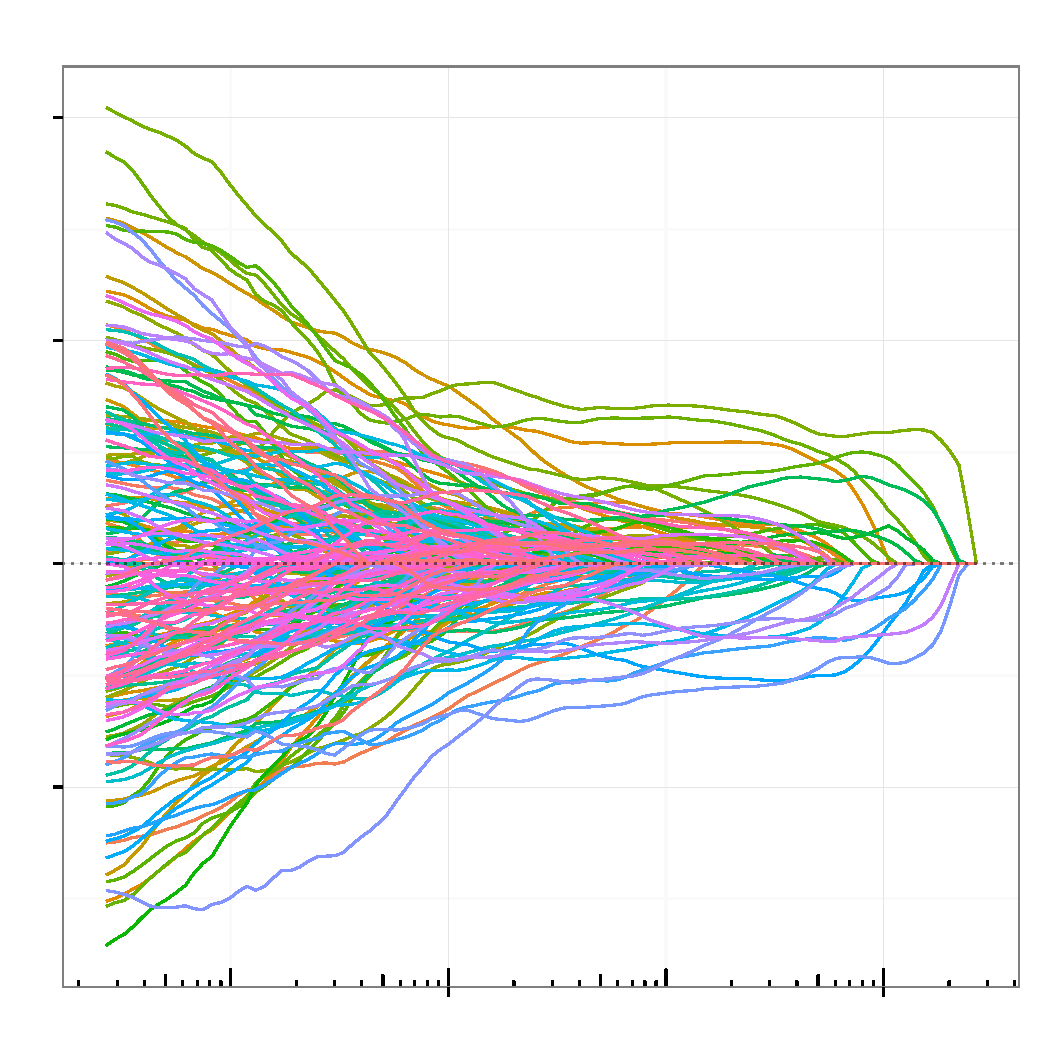
\includegraphics[width=.31\textwidth]{figures/ex_path_lasso}
        & 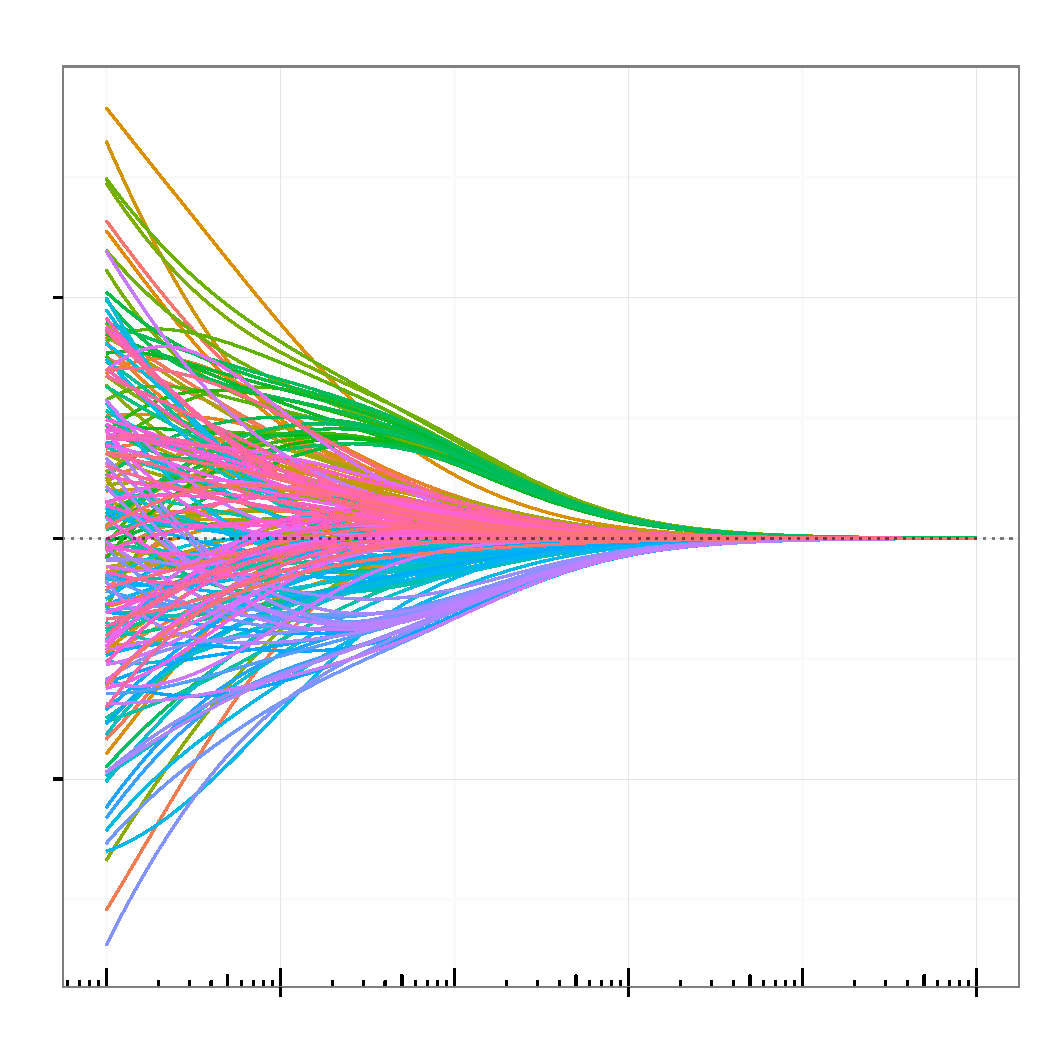
\includegraphics[width=.31\textwidth]{figures/ex_path_ridge}
        & \includegraphics[width=.31\textwidth]{figures/ex_path_breg} \\
        & \multicolumn{3}{c}{small     \hspace{.5cm}      $\longleftarrow$
          \hspace{.5cm} regularization level $\lambda$ (log-scale)
          \hspace{.5cm} $\longrightarrow$ \hspace{.5cm} large}
      \end{tabular}
    \end{small}
    \caption{Regularization paths for the  bridge estimators}
    \label{fig:ex_reg_path}
  \end{figure}

    \end{colormixin}
    \only<2->{
      \vspace{-4.5cm}
      \begin{beamerboxesrounded}[upper=sur:head,lower=sur:bloc,shadow=true]{More structure?}
        How   inducing  broader   types  of   structures?\\

        \alert{Idea}: ``blend'' $\bOmega$ to introduce a broad variety of structures        
      \end{beamerboxesrounded}
    }
  \end{overlayarea}      
  
\end{frame}


\begin{frame}{Accounting for group structures}

  \begin{block}{Group-Lasso norms}
    \vspace{-.5cm}
    \begin{equation*}
      \|   \bbeta   \|_{1,\eta}    =   \sum_{k=1}^K   \omega_k
      \left(\sum_{j\in\group[k]} \beta_j^\eta  \right)^{1/\eta} =
      \sum_{k=1}^K \omega_k \|\bbeta_{\group[k]}\|_\eta.
    \end{equation*}
  \end{block}
  
  \vspace{-.25cm}
  \begin{figure}[htbp!]
    \centering
    \begin{tabular}{@{}ccccc@{}}
      $\ell_{(1,1)}$    &    $\ell_{(2,2)}$   &    $\ell_{(1,4/3)}$    &
      $\ell_{(1,2)}$ \\[1.5ex]
      (Lasso) & (Ridge) & \multicolumn{2}{c}{(Group-Lasso)} & \\ 
      \includegraphics[width=.175\textwidth]{figures/norms_marie/lasso} &
      \includegraphics[width=.175\textwidth]{figures/norms_marie/ridge3D} &
      \includegraphics[width=.175\textwidth]{figures/norms_marie/hierarchical3D} & 
      \includegraphics[width=.175\textwidth]{figures/norms_marie/grouplasso3D} \\
      \includegraphics[width=.175\textwidth]{figures/norms_marie/lasso2D} &
      \includegraphics[width=.175\textwidth]{figures/norms_marie/ridge2D} &
      \includegraphics[width=.175\textwidth]{figures/norms_marie/hierarchical2D} & 
      \includegraphics[width=.175\textwidth]{figures/norms_marie/grouplasso2D} \\
    \end{tabular}
  \end{figure}

\end{frame}

\begin{frame}{Account for direct relationships between the features (I)}
  \framesubtitle{By means of fusion and graph penalties}
  
  \begin{block}{Prior knowledge: a proximity graph $\group[]$ between the variables.}
    \only<1>{A         weighted         graph        $\group[]         =
      (\mathcal{V},\mathcal{E},\mathcal{W})$       with       vertices
      $\mathcal{V}=\set{1,\dots,p}$  and edges  $\mathcal{E}$ weighted
      by             values            $\mathcal{W})=\set{\omega_{ij},
        (i,j)\in\mathcal{E}}$.  
    }
  \end{block}

  \begin{block}{Generalized ``fusion''/total-variation penalty}
    \begin{equation*}
      \sum_{(i,j)\in\mathcal{E}}     \omega_{ij}
      |\beta_i - \beta_j | = \| \bD \bbeta\|_1,
    \end{equation*}
  \end{block}

  \begin{block}{Generalized ridge/Laplacian penalty}
    \begin{equation*}
      \sum_{(i,j)\in\mathcal{E}} \omega_{ij} (\beta_i - \beta_j)^2 =
      \bbeta^\top   \bD^T  \bD   \bbeta   =  \bbeta^\top   \bL  \bbeta   =
      \|\bbeta\|_\bL^2.
    \end{equation*}
  \end{block}
    
\end{frame}

\begin{frame}{Account for direct relationships between the features (II)}
  \framesubtitle{By means of fusion and graph penalties}

  \begin{block}{Example: connected neighbors}
    $\group[]$ is  a chain graph  with edges $\mathcal{E}  = \set{(1,2),
      (2,3), \dots, (p-1,p)}$, and
    \begin{small}
      \begin{equation*}
        \bD =
        \kbordermatrix{
          & 1 & \dots & \dots & p \\
          1 & -1 & 1 & & \\
          \vdots & & \ddots & \ddots \\
          p-1 & & & -1 & 1 \\
        }, \quad
        \bL = \bD^T \bD =
        \kbordermatrix{
          & 1 & \dots & \dots & \dots & p \\
          1 & 1 & -1 & & \\
          \vdots & -1 & 2 & -1 & \ddots \\
          \vdots & & \ddots & \ddots & \ddots\\
          & & & -1 & 2 & 1 \\
          p & & & & -1 & 1 \\
        }.
      \end{equation*}
    \end{small} 
  \end{block}
  
  \begin{block}{``Classical'' TV/fusion penalty}
    \begin{equation*}
      \|\bD\bbeta\|_1 = \sum_{i=1}^{p-1}
      |\beta_{i+1} - \beta_i |, \quad \bbeta^\top \bL \bbeta = \sum_{i=1}^{p-1} (\beta_{i+1} - \beta_i)^2
    \end{equation*}
  \end{block}

\end{frame}

\begin{frame}{Combining several effects}
  \framesubtitle{Typically structure + sparsity}

  \begin{block}{Mixture of penalties}
    For $\alpha\in[0,1]$, consider for instance
    \begin{equation*}
      \begin{array}{rcl}
        \alpha \| \bbeta \|_\gamma & + & (1-\alpha) \| \bbeta \|_\bL^2\\[1ex]
        \alpha \| \bbeta \|_\gamma & + & (1-\alpha) \|\bD \bbeta \|_1.
      \end{array}
    \end{equation*}
  \end{block}

  \begin{figure}[htbp!]
    \centering
    \begin{small}
      \begin{tabular}{@{}c@{\hspace{.2cm}}c@{\hspace{.2cm}}c@{\hspace{.2cm}}c@{\hspace{.2cm}}c@{}}
        $\ell_1 + \ell_2^2$ & $\ell_\infty + \ell_2^2$ & $\ell_1 + \mathrm{TV}$ & $\ell_1 + \ell_2-\mathrm{TV}$ & $\ell_\infty + \ell_2-\mathrm{TV}$\\
        elastic-net & & fused-Lasso & structured enet & \\
        \includegraphics[width=.16\textwidth]{figures/ell1+ell2ball} &
        \includegraphics[width=.16\textwidth]{figures/ellinf+ell2ball} &
        \includegraphics[width=.16\textwidth]{figures/ell1+TVball} & 
        \includegraphics[width=.16\textwidth]{figures/ell1+TVell2ball} & 
        \includegraphics[width=.16\textwidth]{figures/ellinf+ell2TVball}   \\
      \end{tabular}
    \end{small}
    \caption{A couple of examples for various $\alpha$}
    \label{fig:sum_pen}
  \end{figure}
  
\end{frame}


\begin{frame}{Numerical illustration now accounting for structure}
  \framesubtitle{Basic structure integration pays for \alert{interpretability}}

  \begin{small}
    \begin{figure}[htbp!]
      \centering
      \begin{tabular}{@{}c@{}c@{~}c@{~}c@{}}
        &  $\ell_2$--TV  (Laplacian)  &   $\ell_1$  +  $\ell_2$--TV  &
                                                               $\ell_\infty$ + $\ell_2$--TV \\ \rotatebox{90}{\hspace{1.75cm}\small $\hatbbeta_{\lambda,\gamma}$} 
        & \includegraphics[width=.31\textwidth]{figures/ex_path_ridge_str}
        & \includegraphics[width=.31\textwidth]{figures/ex_path_enet_str}
        & \includegraphics[width=.31\textwidth]{figures/ex_path_breg_str} \\
        & \multicolumn{3}{c}{small     \hspace{.5cm}      $\longleftarrow$
          \hspace{.5cm} regularization level $\lambda$ (log-scale)
          \hspace{.5cm} $\longrightarrow$ \hspace{.5cm} large}
      \end{tabular}
      \caption{Regularization paths for the structured estimators}
      \label{fig:ex_reg_path_str}
    \end{figure}
  \end{small}
  
\end{frame}


\begin{frame}
  \frametitle{Variants: the Lasso zoo I}
  \begin{small}
  \begin{block}{The elastic-net (Zou and Hastie, 2005)}
    Tends to activate correlated variables simultaneously:
    \begin{equation*}
      \hat{\bbeta}^{\text{e-net}} = \arg \min_{\bbeta\in \R^p} 
      \left\{\frac{1}{2}\text{RSS}(\bbeta)   +   \lambda   \left(   \alpha
          \|\bbeta \|_1 + (1-\alpha) \|\bbeta\|_2^2 \right) \right\},
    \end{equation*}   
  \end{block}

  \begin{block}{Adaptive/Weighted-Lasso}
    Weights each entry according to a previous estimate e.g. the ols:
    \begin{equation*}
      \hat{\bbeta}^{\text{lasso}} = \arg \min_{\bbeta\in \R^p} 
      \left\{\frac{1}{2}\text{RSS}(\bbeta)  +  \lambda \|\mathbf{w}  \circ
        \bbeta\|_1   \right\},  \quad   \text{with   }  \mathbf{w}   =
      \max\left(1,1/\bbeta^{\mathrm{ols}}\right).
    \end{equation*}
  \end{block}

  \begin{block}{Group-Lasso (Yuan and Lin, 2006)}
  \vspace{-.5cm}
    \begin{equation*}
      \hatbbetagroup = \argmin_{\bbeta\in\mathbb{R}^p} \left\{
        \frac{1}{2}\left\| \mathbf{y} - \mathbf{X}\bbeta \right\|^2 + 
        \lambda \sum_{k=1}^K w_k \left\|\bbeta_{\mathcal{G}_k} \right\| \right\},
    \end{equation*}
  \end{block}
  \end{small}
\end{frame}





\begin{frame}[containsverbatim,allowframebreaks]
\frametitle{Example: prostate cancer}
\framesubtitle{Elastic-net, Adaptive Lasso, Group-Lasso}



\begin{small}
\begin{knitrout}\scriptsize
\definecolor{shadecolor}{rgb}{0.969, 0.969, 0.969}\color{fgcolor}\begin{kframe}
\begin{alltt}
\hlstd{out.elas} \hlkwb{<-} \hlkwd{elastic.net}\hlstd{(x,y,}\hlkwc{lambda2}\hlstd{=}\hlnum{1}\hlstd{)}
\end{alltt}
\end{kframe}
\end{knitrout}

\begin{knitrout}\scriptsize
\definecolor{shadecolor}{rgb}{0.969, 0.969, 0.969}\color{fgcolor}\begin{kframe}
\begin{alltt}
\hlstd{beta.ols} \hlkwb{<-} \hlkwd{lm}\hlstd{(y}\hlopt{~}\hlstd{x)}\hlopt{$}\hlstd{coefficients[}\hlopt{-}\hlnum{1}\hlstd{]}
\hlstd{p.fact} \hlkwb{<-} \hlkwd{pmax}\hlstd{(}\hlnum{1}\hlstd{,}\hlnum{1}\hlopt{/}\hlkwd{abs}\hlstd{(beta.ols))}
\hlstd{out.alasso} \hlkwb{<-} \hlkwd{elastic.net}\hlstd{(x,y,}\hlkwc{penscale}\hlstd{=p.fact)}
\end{alltt}
\end{kframe}
\end{knitrout}

According to the \textsc{Lasso} solution path, we fell like grouping 2
(\texttt{lweight})  and 5 (\texttt{svi}),as  well as  3 (\texttt{age})
and 6 (\texttt{scp}); the same for 4 (\texttt{lbph}) and 8 (\texttt{pgg45}).
\begin{knitrout}\scriptsize
\definecolor{shadecolor}{rgb}{0.969, 0.969, 0.969}\color{fgcolor}\begin{kframe}
\begin{alltt}
\hlstd{group} \hlkwb{<-} \hlkwd{c}\hlstd{(}\hlnum{1}\hlstd{,}\hlnum{2}\hlstd{,}\hlnum{3}\hlstd{,}\hlnum{4}\hlstd{,}\hlnum{2}\hlstd{,}\hlnum{3}\hlstd{,}\hlnum{5}\hlstd{,}\hlnum{4}\hlstd{)}
\hlstd{out.grp} \hlkwb{<-} \hlkwd{group.lasso}\hlstd{(x, y, group)}
\hlstd{sgrp} \hlkwb{<-} \hlkwd{selection}\hlstd{(out.grp)}
\end{alltt}
\end{kframe}
\end{knitrout}
\end{small}

\end{frame}

\begin{frame}[containsverbatim]
\frametitle{Example: prostate cancer}
\framesubtitle{Elastic-net: solution path (penalty)}

\begin{knitrout}\scriptsize
\definecolor{shadecolor}{rgb}{0.969, 0.969, 0.969}\color{fgcolor}
\includegraphics[width=\textwidth]{figures/varLasso-unnamed-chunk-82-1} 

\includegraphics[width=\textwidth]{figures/varLasso-unnamed-chunk-82-2} 

\end{knitrout}
\end{frame}

\begin{frame}[containsverbatim]
\frametitle{Example: prostate cancer}
\framesubtitle{Adaptive-Lasso: solution path (penalty)}

\begin{knitrout}\scriptsize
\definecolor{shadecolor}{rgb}{0.969, 0.969, 0.969}\color{fgcolor}
\includegraphics[width=\textwidth]{figures/varLasso-unnamed-chunk-83-1} 

\includegraphics[width=\textwidth]{figures/varLasso-unnamed-chunk-83-2} 

\end{knitrout}
\end{frame}

\begin{frame}[containsverbatim]
\frametitle{Example: prostate cancer}
\framesubtitle{Group-Lasso: solution path and AIC}

\begin{knitrout}\scriptsize
\definecolor{shadecolor}{rgb}{0.969, 0.969, 0.969}\color{fgcolor}
\includegraphics[width=\textwidth]{figures/varLasso-unnamed-chunk-84-1} 

\end{knitrout}

\end{frame}

\begin{frame}[containsverbatim]
\frametitle{Example: prostate cancer}
\framesubtitle{Group-Lasso: group-norm path and AIC}

\begin{knitrout}\scriptsize
\definecolor{shadecolor}{rgb}{0.969, 0.969, 0.969}\color{fgcolor}
\includegraphics[width=\textwidth]{figures/varLasso-unnamed-chunk-85-1} 

\end{knitrout}

\end{frame}


\subsection{Modèles graphiques gaussiens parcimonieux}

\begin{frame}
  \frametitle{Gaussian Graphical Model: canonical settings}

  \begin{block}{Assays in comparable Gaussian conditions}
    Profiles of  a set  $\mathcal{P} =  \{1,\dots,p\}$ of  variable is
    described by $X\in\mathbb{R}^p$ such as
    \begin{enumerate}
    \item  $X\sim\mathcal{N}(\boldsymbol\mu,\boldsymbol\Sigma)$,  with
      $\boldsymbol\Theta = \bSigma^{-1}$ the precision matrix.
    \item  a  sample $(X^1,  \dots,  X^n)$  of  assays stacked  in  an
      $n\times p$ data matrix $\mathbf{X}$.
    \end{enumerate}
  \end{block}

  \begin{overlayarea}{\textwidth}{\textheight}
    \only<2>{\begin{colormixin}{100!white}}
      \only<1>{\begin{colormixin}{40!white}}
        
        \begin{block}{Conditional independence structure}
          \vspace{-.5cm}
          \begin{equation*}
            (i,j)  \notin  \mathcal{E}  \Leftrightarrow  X_i  \indep  X_j  |
            X_{\backslash \{i,j\}} \Leftrightarrow \Theta_{ij} = 0.
          \end{equation*}
        \end{block}
        
        \vspace{-.5cm}
        \begin{block}{Graphical interpretation}
          \vspace{-.5cm}
          \begin{center}
            \begin{tabular}{c@{\hspace{2cm}}c}
              \begin{tabular}{c}
                \small $\mathcal{G}=(\mathcal{P},\mathcal{E})$ \\
                \includegraphics[width=.3\textwidth]{graph}
              \end{tabular}
              &
              \begin{tabular}{c}
                \small $\bTheta$\\\includegraphics[width=.2\textwidth]{Markovadjacency}
              \end{tabular}
            \end{tabular}
          \end{center}
        \end{block}
        \vspace{-1cm}
        $\rightsquigarrow$ \alert{``Covariance'' selection}
  
      \end{colormixin}

      \only<1>{
        \vspace{-4cm}      
        \begin{beamerboxesrounded}[upper=sur:head,lower=sur:bloc,shadow=true]{The data}
          Stacking    $(X^1,\dots,    X^n)$,    we   met    the    usual
          individual/variable table $\mathbf{X}$

        \begin{tikzpicture}
          \node[opacity=.75] at (-3,1.5) {\pgfuseimage{microarray}};
          \node[opacity=.9] at (-2.75,1.25) {\pgfuseimage{microarray}};
          \node[opacity=.95] at (-2.5,1) {\pgfuseimage{microarray}};
          \node at (-2.25,0.75) {\pgfuseimage{microarray}};
          \node[fill=red, text=white,single arrow] 
          (inference) at (0,1) {\sf \scriptsize stacked in}; 
          
          \node at (4.5,1) {%
            $\mathbf{X} = \begin{pmatrix} 
              x_1^1 & x_1^2 & x_1^3 & \dots & x_1^p \\
              \vdots \\
              x_n^1 & x_n^2 & x_1^2 & \dots & x_n^p \\
            \end{pmatrix}$};
        \end{tikzpicture}
      \end{beamerboxesrounded}
    }
  \end{overlayarea}      
\end{frame}

\begin{frame}
  \frametitle{Gold standard penalized approaches}
  \framesubtitle{Use $\ell_1$ for both regularizing and promoting \textit{sparsity}}

  \begin{overlayarea}{\textwidth}{\textheight}
    \only<1-3>{\begin{colormixin}{100!white}}
      \only<4->{\begin{colormixin}{40!white}}

  \begin{block}{Penalized likelihood (Banerjee \textit{et al.}, Yuan and Lin, 2008)}
    \vspace{-1em}
    \begin{equation*}
      \hat{\bTheta}_\lambda=\argmax_{\bTheta \in \mathbb{S}_+}
      \ell(\bTheta;\mathbf{X})-\lambda
      \|\bTheta\|_{1}
    \end{equation*}
  \end{block}
  \vspace*{-1em}

  \only<1>{
    \begin{itemize}
    \item[\textcolor{green}{$+$}] symmetric, positive-definite
    \item[\textcolor{red}{$-$}] solved by the ``Graphical-Lasso''
      ($\mathcal{O}(p^3)$, \textit{Friedman et al, 2007}).
    \end{itemize}
  }

  \vfill

  \begin{block}{Neighborhood Selection (Meinshausen \& B\"ulhman, 2006)}<2->
    \vspace*{-1em}
    \begin{equation*}
      \widehat{\boldsymbol\beta}^{(i)} = \argmin_{\boldsymbol\beta \in \mathbb{R}^{p-1} }
      \frac{1}{n} \left\| \mathbf{X}_i - \mathbf{X}_{\backslash i} \,
        {\boldsymbol\beta} \right\|_2^2 + \lambda \left\| {\boldsymbol\beta} \right\|_{1}
    \end{equation*}
    \vspace*{-0.75\baselineskip}
  \end{block}
  
  \only<2>{
    \begin{itemize}
    \item[\textcolor{red}{$-$}] not symmetric, not positive-definite
    \item[\textcolor{green}{$+$}] $p$
      Lasso solved with Lars-like algorithms ($\mathcal{O}(npd)$ for $d$ neighbors).
    \end{itemize}
  }

  \begin{block}{CLIME -- Pseudo-likelihood (Cai et al., 2011; Yuan, 2010)}<3->
    \vspace*{-1em}
    \begin{equation*}
      \widehat{\boldsymbol\Theta} = \argmin_{\boldsymbol\Theta}
      \left\|   {\boldsymbol\Theta} \right\|_1 \text{ subjected to }
      \left\|    n^{-1}\mathbf{X}^t     \mathbf{X}    \boldsymbol\Theta    -
        \mathbf{I} \right\|_\infty\leq \lambda
    \end{equation*}
    \vspace*{-0.75\baselineskip}
  \end{block}

  \only<3>{
    \begin{itemize}
    \item[\textcolor{red}{$-$}] not positive-definite
    \item[\textcolor{green}{$+$}]    $p$   linear    programs   easily
      distributed ($\mathcal{O}(p^2d)$ for $d$ neighbors).
    \end{itemize}
  }
  
  \end{colormixin}

  \only<4>{
    \vspace{-4cm}      
    \begin{beamerboxesrounded}[upper=sur:head,lower=sur:bloc,shadow=true]{Variants
        and recent improvements}
      
      '13 NIPS submissions
      \begin{itemize}
      \item  Use  square-root  Lasso  in place  of  Lasso  for  tuning
        insensitive property package
      \item Solve CLIME for $p=10^6$ (on 400 cores).
      \end{itemize}
        
      See   \texttt{R}   package  \texttt{huge},   \texttt{fastclime},
      \texttt{flare}, \texttt{QUIC}.
    \end{beamerboxesrounded}
  }

\end{overlayarea}      

\end{frame}

\begin{frame}[containsverbatim,allowframebreaks]
\frametitle{Estimating the covariance structure of the plasmodium data}

\begin{knitrout}\scriptsize
\definecolor{shadecolor}{rgb}{0.969, 0.969, 0.969}\color{fgcolor}\begin{kframe}
\begin{alltt}
\hlkwd{library}\hlstd{(Matrix)}
\hlkwd{load}\hlstd{(}\hlstr{"plasmodium_expression.Rdata"}\hlstd{)}
\hlkwd{dim}\hlstd{(Y)}
\end{alltt}
\begin{verbatim}
## [1] 3490   46
\end{verbatim}
\begin{alltt}
\hlkwd{head}\hlstd{(Y)[,} \hlnum{1}\hlopt{:}\hlnum{5}\hlstd{]}
\end{alltt}
\begin{verbatim}
##                TP1    TP2    TP3    TP4    TP5
## MAL13P1.100 0.4510 0.6532 1.0760 0.5515 0.4238
## MAL13P1.102 1.5320 1.8920 0.8803 1.0300 0.9328
## MAL13P1.103 0.5218 0.5213 0.5328 0.3719 0.3258
## MAL13P1.105 0.5515 0.5527 0.8627 0.4541 0.4299
## MAL13P1.107 0.5630 0.4463 1.0760 0.4035 0.2082
## MAL13P1.112 0.5390 0.5393 0.5642 0.5326 0.4469
\end{verbatim}
\begin{alltt}
\hlkwd{image}\hlstd{(}\hlkwd{Matrix}\hlstd{(}\hlkwd{cor}\hlstd{(Y)))}
\end{alltt}
\end{kframe}
\includegraphics[width=\textwidth]{figures/ggm-unnamed-chunk-86-1} 

\end{knitrout}
\end{frame}


\begin{frame}[containsverbatim,allowframebreaks]
\frametitle{Estimating the covariance structure}
\framesubtitle{Sparse Estimation}

\begin{knitrout}\scriptsize
\definecolor{shadecolor}{rgb}{0.969, 0.969, 0.969}\color{fgcolor}\begin{kframe}
\begin{alltt}
\hlkwd{library}\hlstd{(huge)}
\hlstd{huge.out} \hlkwb{<-} \hlkwd{huge}\hlstd{(}\hlkwd{as.matrix}\hlstd{(Y),} \hlkwc{method}\hlstd{=}\hlstr{"glasso"}\hlstd{,} \hlkwc{cov.output}\hlstd{=}\hlnum{TRUE}\hlstd{)}
\end{alltt}
\begin{verbatim}
## Conducting the graphical lasso (glasso) with lossless screening....in progress:0% 
Conducting the graphical lasso (glasso) with lossless screening....in progress:9% 
Conducting the graphical lasso (glasso) with lossless screening....in progress:19% 
Conducting the graphical lasso (glasso) with lossless screening....in progress:30% 
Conducting the graphical lasso (glasso) with lossless screening....in progress:40% 
Conducting the graphical lasso (glasso) with lossless screening....in progress:50% 
Conducting the graphical lasso (glasso) with lossless screening....in progress:60% 
Conducting the graphical lasso (glasso) with lossless screening....in progress:70% 
Conducting the graphical lasso (glasso) with lossless screening....in progress:80% 
Conducting the graphical lasso (glasso)....done.                                          
\end{verbatim}
\begin{alltt}
\hlstd{sel.out}  \hlkwb{<-} \hlkwd{huge.select}\hlstd{(huge.out)}
\end{alltt}
\begin{verbatim}
## Conducting extended Bayesian information criterion (ebic) selection....done
\end{verbatim}
\begin{alltt}
\hlkwd{image}\hlstd{(sel.out}\hlopt{$}\hlstd{opt.cov)}
\end{alltt}
\end{kframe}
\includegraphics[width=\textwidth]{figures/ggm-unnamed-chunk-87-1} 

\end{knitrout}
\end{frame}

\begin{frame}[containsverbatim,allowframebreaks]
\frametitle{Estimating the covariance structure}
\framesubtitle{Sparse Estimation of the inverse covariance}

\begin{knitrout}\scriptsize
\definecolor{shadecolor}{rgb}{0.969, 0.969, 0.969}\color{fgcolor}\begin{kframe}
\begin{alltt}
\hlkwd{sum}\hlstd{(}\hlkwd{abs}\hlstd{(sel.out}\hlopt{$}\hlstd{opt.icov)} \hlopt{!=} \hlnum{0}\hlstd{)}
\end{alltt}
\begin{verbatim}
## [1] 760
\end{verbatim}
\begin{alltt}
\hlkwd{ncol}\hlstd{(sel.out}\hlopt{$}\hlstd{opt.icov)} \hlopt{**} \hlnum{2}
\end{alltt}
\begin{verbatim}
## [1] 2116
\end{verbatim}
\begin{alltt}
\hlkwd{image}\hlstd{(sel.out}\hlopt{$}\hlstd{opt.icov)}
\end{alltt}
\end{kframe}
\includegraphics[width=\textwidth]{figures/ggm-unnamed-chunk-88-1} 

\end{knitrout}

\end{frame}

\end{document}

